%% OSDI -- 12 pages limit
\documentclass[letterpaper,twocolumn,10pt]{article}
\usepackage{usenix2019_v3}


%% For double-blind review submission, w/o CCS and ACM Reference (max submission space)
% Limit: 25 pages
% https://icfp20.sigplan.org/track/icfp-2020-papers#Call-for-Papers
%% \documentclass[acmsmall,10pt,review,anonymous]{acmart}
%% \settopmatter{printfolios=false,printccs=false,printacmref=false}
%% For double-blind review submission, w/ CCS and ACM Reference
%\documentclass[sigplan,review,anonymous]{acmart}\settopmatter{printfolios=true}
%% For single-blind review submission, w/o CCS and ACM Reference (max submission space)
%\documentclass[sigplan,review]{acmart}\settopmatter{printfolios=true,printccs=false,printacmref=false}
%% For single-blind review submission, w/ CCS and ACM Reference
%\documentclass[sigplan,review]{acmart}\settopmatter{printfolios=true}
%% For final camera-ready submission, w/ required CCS and ACM Reference
%\documentclass[sigplan]{acmart}\settopmatter{}

% \acmSubmissionID{248}

\usepackage{enumitem}
\usepackage{booktabs}
\usepackage{amssymb}
\usepackage{soul}
\usepackage{xspace}
\usepackage{color}
\usepackage{xcolor}
\usepackage{upquote}
\usepackage{listings}
\usepackage{amsmath}
\usepackage{cleveref}
\usepackage{wrapfig}
\usepackage{syntax}
\usepackage{caption}

\usepackage{tikz}
\usetikzlibrary{arrows,automata,shapes.misc,shapes.geometric,positioning}

\captionsetup[figure]{font=footnotesize,name={Fig.},labelfont={bf, footnotesize}}
\captionsetup[table]{font=footnotesize,name={Tab.},labelfont={bf, footnotesize}, skip=2pt, aboveskip=2pt}
\captionsetup{font=footnotesize,labelfont={bf, footnotesize}, belowskip=2pt}

\newcommand{\eg}{{\em e.g.}, }
\newcommand{\ie}{{\em i.e.}, }
\newcommand{\etc}{{\em etc.}\xspace}
\newcommand{\vs}{{\em vs.} }
\newcommand{\cmpn}{compartmentalization} 
\newcommand{\heading}[1]{\vspace{4pt}\noindent\textbf{#1}\enspace}
\newcommand{\ttt}[1]{\texttt{#1}}
\newcommand{\ttiny}[1]{\texttt{\scriptsize #1}}
\newcommand{\tti}[1]{\texttt{\scriptsize #1}}
\newcommand{\spol}[1]{\scriptsize{\sc#1}}
\newcommand{\pol}[1]{\texttt{\small {\color{purple}#1}}}
\newcommand{\rf}[1]{\ref{#1}}
\newcommand{\wka}{\ttt{a\textsubscript{1}}}
\newcommand{\wkq}{\ttt{q\textsubscript{1-4}}}

\newcommand{\cn}[1]{\mbox{\textcircled{\footnotesize #1}}}
\newcommand{\tcn}[1]{\mbox{\textcircled{\scriptsize #1}}}

\newcommand{\sta}{\cn{\textsc{S}}\xspace}
\newcommand{\pur}{\cn{\textsc{P}}\xspace}
\newcommand{\npu}{\cn{\textsc{N}}\xspace}
\newcommand{\sid}{\cn{\textsc{E}}\xspace}
\newcommand{\dfs}{\cn{\textsc{F}}\xspace}
\newcommand{\irr}{\cn{\textsc{I}}\xspace}

\newcommand{\tsta}{\tcn{\textsc{S}}\xspace}
\newcommand{\tpur}{\tcn{\textsc{P}}\xspace}
\newcommand{\tnpu}{\tcn{\textsc{N}}\xspace}
\newcommand{\tsid}{\tcn{\textsc{E}}\xspace}
\newcommand{\tirr}{\tcn{\textsc{I}}\xspace}
\newcommand{\tdfs}{\tcn{\textsc{F}}\xspace}

% For comments
\newcommand{\eat}[1]{}
\newcommand{\TODO}[1]{\hl{\textbf{TODO:} #1}\xspace}
\newcommand{\todo}[1]{\hl{#1}\xspace}
\newcommand{\fixme}[1]{[{\color{red}#1}]}
\newcommand{\nv}[1]{[{\color{cyan}nv: #1}]}
\newcommand{\kk}[1]{[{\color{magenta}kk: #1}]}
\newcommand{\km}[1]{[{\color{blue}km: #1}]}
\newcommand{\review}[1]{{\color{red}#1}}
\newcommand{\tr}[1]{} %% Text and comments for technical report

\newcommand{\kstar}{^{\textstyle *}}
\newcommand{\eps}{\varepsilon}

\definecolor{editorGray}{rgb}{0.95, 0.95, 0.95}
\definecolor{editorOcher}{rgb}{1, 0.5, 0} % #FF7F00 -> rgb(239, 169, 0)
\definecolor{editorGreen}{rgb}{0, 0.5, 0} % #007C00 -> rgb(0, 124, 0)

\definecolor{cdb}{rgb}{0.37, 0.62, 0.63} % cadet blue

\lstdefinelanguage{sh}{
  morekeywords={for, in, do, done, \|},
  keywordstyle=\color{purple}\ttfamily,
  % ndkeywords={curl, grep, wget, awk, xargs, find, nc, mdc, gunzip, cut, sort, head, join},
  ndkeywordstyle=\color{black}\ttfamily\bfseries,
  identifierstyle=\color{black},
  sensitive=false,
  comment=[l]{\#},
  commentstyle=\color{lightgray},
% morecomment=[s]{/\\*\\*, \\*/},
  stringstyle=\color{darkgray}\ttfamily,
  morestring=[b]',
  morestring=[b]",
% numbersep=1pt,
% numberstyle=\footnotesize\bf\color{gray},   % the style that is used for the line-numbers
  abovecaptionskip=0pt,
  aboveskip=0pt,
  belowcaptionskip=0pt,
  belowskip=0pt,
  frame=none                     % adds a frame around the code
% moredelim=[s][\color{gray}]{c:}{>},
% moredelim=[s][\color{orange}]{/*}{/}
}

\lstset{ %
  backgroundcolor=\color{white},   % choose the background color; you must add \usepackage{color} or \usepackage{xcolor}
  basicstyle=\normalsize\ttfamily,  % the size of the fonts that are used for the code
  upquote=true,
  captionpos=b,                    % sets the caption-position to bottom
% frame=B,                    % adds a frame around the code
  numbers=left,                    % where to put the line-numbers; possible values are (none, left, right)
  numbersep=2pt,                   % how far the line-numbers are from the code
  numberstyle=\tiny\color{gray},   % the style that is used for the line-numbers
  rulecolor=\color{black},         % if not set, the frame-color may be changed on line-breaks within not-black text (e.g. comments (green here))
  framerule=0pt,
	xleftmargin=0pt,
	xrightmargin=0pt,
	breakindent=0pt,
  aboveskip=0pt,
  framesep=0pt,
  abovecaptionskip=0pt,
  aboveskip=0pt,
  belowcaptionskip=0pt,
  belowskip=0pt,
  frame=none,
  framexbottommargin=0pt,
  resetmargins=true
}



%% Conference information
%% Supplied to authors by publisher for camera-ready submission;
%% use defaults for review submission.
%% \acmConference[PL'18]{ACM SIGPLAN Conference on Programming Languages}{January 01--03, 2018}{New York, NY, USA}
%% \acmYear{2018}
%% \acmISBN{} % \acmISBN{978-x-xxxx-xxxx-x/YY/MM}
%% \acmDOI{} % \acmDOI{10.1145/nnnnnnn.nnnnnnn}
%% \startPage{1}

%% Copyright information
%% Supplied to authors (based on authors' rights management selection;
%% see authors.acm.org) by publisher for camera-ready submission;
%% use 'none' for review submission.
%% \setcopyright{none}
%\setcopyright{acmcopyright}
%\setcopyright{acmlicensed}
%\setcopyright{rightsretained}
%\copyrightyear{2018}           %% If different from \acmYear

%% Bibliography style
\bibliographystyle{plain}
%% Citation style
%\citestyle{acmauthoryear}  %% For author/year citations
%\citestyle{acmnumeric}     %% For numeric citations
%\setcitestyle{nosort}      %% With 'acmnumeric', to disable automatic
                            %% sorting of references within a single citation;
                            %% e.g., \cite{Smith99,Carpenter05,Baker12}
                            %% rendered as [14,5,2] rather than [2,5,14].
%\setcitesyle{nocompress}   %% With 'acmnumeric', to disable automatic
                            %% compression of sequential references within a
                            %% single citation;
                            %% e.g., \cite{Baker12,Baker14,Baker16}
                            %% rendered as [2,3,4] rather than [2-4].


%%%%%%%%%%%%%%%%%%%%%%%%%%%%%%%%%%%%%%%%%%%%%%%%%%%%%%%%%%%%%%%%%%%%%%
%% Note: Authors migrating a paper from traditional SIGPLAN
%% proceedings format to PACMPL format must update the
%% '\documentclass' and topmatter commands above; see
%% 'acmart-pacmpl-template.tex'.
%%%%%%%%%%%%%%%%%%%%%%%%%%%%%%%%%%%%%%%%%%%%%%%%%%%%%%%%%%%%%%%%%%%%%%


%% Some recommended packages.
\usepackage{booktabs}   %% For formal tables:
                        %% http://ctan.org/pkg/booktabs
\usepackage{subcaption} %% For complex figures with subfigures/subcaptions
                        %% http://ctan.org/pkg/subcaption

\begin{document}

%% Title information
%% \title{Dish: Distribution-oblivious Shell Scripting}         %% [Short Title] is optional;
\title{\sys: Light-touch Data-Parallel Shell Processing}         %% [Short Title] is optional;
%% \title{Extensible data processing in the shell}

% \titlenote{with title note}             %% \titlenote is optional;
%                                         %% can be repeated if necessary;
%                                         %% contents suppressed with 'anonymous'
% \subtitle{Subtitle}                     %% \subtitle is optional
% \subtitlenote{with subtitle note}       %% \subtitlenote is optional;
                                        %% can be repeated if necessary;
                                        %% contents suppressed with 'anonymous'

%% Author information
%% Contents and number of authors suppressed with 'anonymous'.
%% Each author should be introduced by \author, followed by
%% \authornote (optional), \orcid (optional), \affiliation, and
%% \email.
%% An author may have multiple affiliations and/or emails; repeat the
%% appropriate command.
%% Many elements are not rendered, but should be provided for metadata
%% extraction tools.

%% Author with single affiliation.
\author{
  Anonymous Author(s)\\
  \normalsize{Additional Anonymized Material: \href{https://git.io/JfEgr}{https://git.io/JfEgr}.}
}
%% \authornote{with author1 note}          %% \authornote is optional;
%%                                         %% can be repeated if necessary
%% \orcid{nnnn-nnnn-nnnn-nnnn}             %% \orcid is optional
%% \affiliation{
%%   \position{Position1}
%%   \department{Department1}              %% \department is recommended
%%   \institution{Institution1}            %% \institution is required
%%   \streetaddress{Street1 Address1}
%%   \city{City1}
%%   \state{State1}
%%   \postcode{Post-Code1}
%%   \country{Country1}                    %% \country is recommended
%% }
%% \email{first1.last1@inst1.edu}          %% \email is recommended

%% Author with two affiliations and emails.
% \author{First2 Last2}
%% \authornote{with author2 note}          %% \authornote is optional;
%%                                         %% can be repeated if necessary
%% \orcid{nnnn-nnnn-nnnn-nnnn}             %% \orcid is optional
%% \affiliation{
%%   \position{Position2a}
%%   \department{Department2a}             %% \department is recommended
%%   \institution{Institution2a}           %% \institution is required
%%   \streetaddress{Street2a Address2a}
%%   \city{City2a}
%%   \state{State2a}
%%   \postcode{Post-Code2a}
%%   \country{Country2a}                   %% \country is recommended
%% }
%% \email{first2.last2@inst2a.com}         %% \email is recommended
%% \affiliation{
%%   \position{Position2b}
%%   \department{Department2b}             %% \department is recommended
%%   \institution{Institution2b}           %% \institution is required
%%   \streetaddress{Street3b Address2b}
%%   \city{City2b}
%%   \state{State2b}
%%   \postcode{Post-Code2b}
%%   \country{Country2b}                   %% \country is recommended
%% }
%% \email{first2.last2@inst2b.org}         %% \email is recommended

\newcommand{\cf}[1]{(\emph{Cf}.\S\ref{#1})}
\newcommand{\sx}[1]{(\S\ref{#1})}
\newcommand{\sys}{{\scshape PaSh}\xspace}
\newcommand{\unix}{{\scshape Unix}\xspace}

\setlist{noitemsep,leftmargin=10pt,topsep=2pt,parsep=2pt,partopsep=2pt}



%% 2012 ACM Computing Classification System (CSS) concepts
%% Generate at 'http://dl.acm.org/ccs/ccs.cfm'.
%% \begin{CCSXML}
%% <ccs2012>
%% <concept>
%% <concept_id>10011007.10011006.10011008</concept_id>
%% <concept_desc>Software and its engineering~General programming languages</concept_desc>
%% <concept_significance>500</concept_significance>
%% </concept>
%% <concept>
%% <concept_id>10003456.10003457.10003521.10003525</concept_id>
%% <concept_desc>Social and professional topics~History of programming languages</concept_desc>
%% <concept_significance>300</concept_significance>
%% </concept>
%% </ccs2012>
%% \end{CCSXML}

%% \ccsdesc[500]{Software and its engineering~General programming languages}
%% \ccsdesc[300]{Social and professional topics~History of programming languages}
%% End of generated code


%% Keywords
%% comma separated list
% \keywords{keyword1, keyword2, keyword3}  %% \keywords are mandatory in final camera-ready submission


%% \maketitle
%% Note: \maketitle command must come after title commands, author
%% commands, abstract environment, Computing Classification System
%% environment and commands, and keywords command.
\maketitle

%% Abstract
%% Note: \begin{abstract}...\end{abstract} environment must come
%% before \maketitle command
\begin{abstract}
  This paper presents \sys, a shell aimed at parallelizing POSIX shell scripts through a combination of program transformations and runtime primitives.
  Given a script, \sys converts it to a data-flow graph, performs a series of analyses that aim at exposing parallelism while preserving its sequential semantics, and then converts it back to a script that uses POSIX constructs to explicitly guide parallelism.
A set of lightweight annotations allow command developers to express key parallelizability properties of their commands.
An accompanying pararllelizability study of commands in POSIX and GNU Coreutils, two large and commonly used groups, 
informs \sys's annotation language and result in its equivalent of a data-parallel standard library.
Finally, \sys's \unix-aware runtime primitives address several practical issues related to performance and correctness.
\sys's extensive evaluation, combining several classic and modern Unix scripts, shows significant benefits across several axes—with order-of-maginute performance improvements stemming from the combination of its program transformations and runtime primitives.
\end{abstract}

% Its runtime component provides orchestration and planning support during the execution of the program.
% These are from the abstract:
%  with regards to the sequential program.
  % leveraging the insight that such programs already express stream computations, with their stages falling under a few, known parallelizability classes.
% a series of techniques for automatically 
% 
% Key challenges include 
% surprisingly expressive, 
% maximally distributable subprograms
% 


\section{Introduction}
\label{intro}


% \TODO{Drop the automated from the title maybe?}
% \nv{Updates}

%% \kk{After discussion on Wednesday Jan 8: Modify the narrative of
%%   this paper to talk about data processing in the Shell. Make this
%%   the main focus of the paper. This simplifies the narrative and
%%   allows us to not talk about late planner activation as well as
%%   environment variables. It also justifies why we only deal with
%%   pure and stateless. Note that this is a very expressive model, as
%%   shown by our benchmark suite. Note: Rememeber to clearly describe
%%   the subset of the shell that we handle. To be more precise the
%%   compositional operator of the shell that we can handle.}

%% \kk{Note: A point that we need to establish early on and convince
%%   the readers about is that the Shell IS used already for
%%   data-processing, and that we are not just proposing it as an
%%   alternative to other systems. We do not propose migrating to
%%   shell scripts if you already have a parallel/efficient
%%   solution. I am not sure if that needs a specific paragraph of its
%%   own at the start of the introduction. Like: ``Consider the
%%   following bash script that does some simple data
%%   processing... Examples like that exists in several
%%   domains/applications (examples, cite).''}


%% \kk{Decide if we will mainly focus on scripts or pipelines and
%%   choose wordings appropriately.}
%
% Consider the following data processing Shell script.
% %% \kk{We might want to have a more complex script here.}
% 
% \begin{lstlisting}[language=sh, float=h, numbers=none, escapeinside={($}{$)}]
% cat * | tr -cs A-Za-z\n | tr A-Z a-z |    ($$(p_1)$$)
%   sort | uniq -c | sort -rn | head 5 > out
% \end{lstlisting}
% 
% \noindent
% great sentence -- keep
% Scripts like the one above are commonly used for orchestrating data-processing workflows; connecting system commands with custom tools to perform complex tasks.
% %% \kk{Do we need to mention domains where that happens?}
% Even though shell pipelines are designed to exploit task parallelism, they completely ignore available data-parallelism.
% % Too low-level descriptions of the problem, maybe keep it high level?
% For small input sizes this isn't a problem since scripts take less than a second to execute, but as data sizes increase, failing to utilize the underlying parallel computational resources is a significant bottleneck.

The \unix shell is an environment---often interactive---for composing scripts written in a plethora of programming languages.
This language-agnosticism, coupled with \unix's toolbox philosophy~\cite{mcilroy1978unix}, makes the shell the primary choice for specifying succinct and simple pipelines that target data processing, system orchestration, and other automation tasks.
% Pipe-centric shell commands are parallel (and to some extent, functional) programs that can natively enjoy significant parallelism on a multicore machine.
Unfortunately, parallelizing such pipelines requires significant effort shared between two different programmer groups. % it's more like roles personas or "wearing hats"

The first group is \emph{command developers}, responsible for developing individual commands such as \ttt{sort}, \ttt{uniq}, and \ttt{jq}.
These developers usually work in a single programming language, leveraging its abstractions to provide parallelism whenever possible.
As they have no visibility into the command's uses, they expose a plethora of ad-hoc command-specific flags such as \ttt{-t}, \ttt{-}\ttt{-parallel}, \ttt{-p}, and \ttt{-j} % , \ttt{CPUs}, and \ttt{NUM\_THREADS}~\cite{}.
\cite{pasetto2011comparative, mcilroy1993engineering, stallman1991gnu}.

The second group is \emph{shell users}, who use POSIX shell constructs to combine multiple such commands from many languages into their scripts and are thus left with only a few options for incorporating parallelism.
% \kk{I don't really like the reference to such a later section. Can we remove it?}
% \nv{We have to say this is not just ``an opinion'', but that we give a scientific treatment/full coverage in the related work section. How far away should the sections be so that you're comfortable referencing to?}
% If versed into parallelism, 
% Users versed in computing can apply 
% these tools are command-unaware thus at risk of breaking program semantics,
% require manual changes to the code to make parallelism explicit,
% at times leverage command flags like the ones mentioned earlier---but each command 
% oblivious? agnostic?  
One option is manual tools such GNU \ttt{parallel}~\cite{Tange2011a}, \ttt{ts}~\cite{tsp}, \ttt{qsub}~\cite{gentzsch2001sun}, \textsc{SLURM}~\cite{yoo2003slurm};
  these tools are either command-unaware thus at risk of breaking program semantics, or too coarse-grained thus only being capable to exploit parallelism at the level of entire scripts rather than individual components.
% Tools will attempt to parallelize anything 
% use the composition abstractions of the \unix shell, 
% and are often prototypical in nature---focusing on quickly prototyping a solution for the task at hand rather building an optimal solution to a recurring pattern.
% short lived, changing quickly
% (ii) ad-hoc flags provided by command developers and mentioned above.
Another option is to use shell primitives such as \ttt{\&}, \ttt{wait}, \ttt{for} to explicitly induce concurrency;
 these come at a cost of manual effort to split inputs, rewrite scripts, and orchestrate execution---an expensive and error-prone process.
% re-writing of the entire script from scratch; unfortunately, this process is expensive and can introduce new bugs, cascading changes, and divergence from legacy functionality---but also foregoes all the productivity benefits of the original script.
% The fact that a programmer often belongs to both groups at the same time---as composed scripts can themselves form a command used in other scrips---compounds the challenge.
To top it off, all these options assume a good understanding of parallelism;
  users whose domain of expertise falls outside computing---routinely writing shell scripts to accomplish their tasks---are left without options (see~\S\ref{related} for a full discussion).
% \nv{I still don't like ``for a full discussion''---raises too many expectations, and we don't have that much more to say}

To address this challenge, we develop \sys, a shell that parallelizes POSIX shell scripts. \kk{We need to mention data-parallelism earlier. We don't focus on general parallelization but rather data-parallelism (performing operations on disjoint partitions of the input and then merging the results. WE need to give a brief idea about that early on so that we don't create false ideas.}
% \kk{Mention that it outputs shell scripts.}
% \nv{I think the ``how'' it solves it should come later, we're still trying to convince them we solve it (see next sentences in this paragraph)
% \sys offers both classes of users in the second group such much-needed automation.
\sys benefits both programmer groups mentioned earlier, with a particular emphasis on users.
Command developers are provided a set of abstractions, akin to lightweight type annotations, for expressing the parallelizability properties of their commands:
  rather than providing a command's full observable behavior, these annotations focus primarily on their interaction with state.
Shell users, on the other hand, are provided full automation:
  \sys extracts parallelism latent in their scripts by analyzing their parallelizability properties. % of their fragments.
% benefiting scripting experts and non-experts alike by offering automated POSIX-aware parallelization of shell-scripts as long as command developers
\sys's transformations are conservative, in that they do not attempt to parallelize fragments that lack sufficient information---\ie at worst, \sys will choose to not improve performance rather than risking breakage.
% \kk{Should we mention that we only show this empirically?}
% \nv{I don't think so; I don't think this is the right point to talk about our evaluation, we just state our intention/high-level principles.}

To address cold-start issues, \sys comes with a library of parallelizability semantics for commands in POSIX and GNU Coreutils.
These large classes of commands serve as the shell's standard library, expected to be found pervasively. % in scripts found out in the wild.
The study that led to their characterization also informed \sys's annotation and transformation components.\footnote{
  In fact, the scope of the study is broader, incorporating also commands outside POSIX and GNU Coreutils such as \ttt{curl} and \ttt{pandoc}.
}

These components are finally paired with \sys's runtime component.
% \sys's runtime  component additional packs
% Aside from these two components, \sys packs a runtime component that serves dual purpose:
Aware of the \unix philosophy and abstractions, it packs a small library of highly-optimized data combinators as well as high-performance primitives for eager data splitting and merging.
These address several practical challenges % such as task parallelism, deadlocks, and performance bottlenecks,
  and were developed by uncovering several pathological situations, on many of which we report.


%% First, shell users composing pipelines (or simply running legacy pipelines on massive datasets) can see scalability benefits without any manual effort---no need for \ttt{qsub}~\cite{gentzsch2001sun}, \textsc{SLURM}~\cite{yoo2003slurm}, calls to \textsc{GNU} \ttt{parallel}~\cite{Tange2011a}, or any manual rewriting~\cite{mapreduce:08, ciel:11, spark:12}.

% \sys packs several ideas around the insight that a large subset of the Shell language can be represented as a dataflow graph, enabling for parallelization optimizations.
% First, a careful study of the parallelizability properties of shell primitives and commands.
% \sys addresses the challenge by offering command developers a unified set of abstractions for describing the parallelizability characteristics of their commands.
% Using lightweight annotations akin to type signatures, \sys can automate the parallelization of entire POSIX scripts without any input from their user.
% hand-in-hand with the parallelizability study:
%   the study informed the annotation language and was used to annotate the entire
%   for all 
% ---a set of annotations that \sys already offers for 
% for the standard library
%   akin to the standard library
%   the annotation language is informed by the study, but also the study is 
% XX to a type signature, these annotations describe 
% 
% Second, \sys defines a dataflow graph model that is suitable for the semantics of the POSIX shell and proposes a set of parallelization optimizations that preserve the behavior of the dataflow graph.
% (one sentence for the model)
% (one sentence for the optimizations)
% The result of the compilation is still a POSIX-compliant script that manages parallelism explicitly;
%   POSIX compliance means 
% it does not depend on a managed runtime 
% 
% Third, \sys packs a runtime component 
% A small library of highly-optimized data combiners allows 
% This is paired with a
% it comes with a few runtime primitives for eager data splitting and merging that address several practical issues ranging from deadlocks, performance bottlenecks;
%   these primitives were developed from uncovering several pathological situations, on many of which we report.

We evaluate \sys using
  (i) a series of benchmarks, ranging from classic one-liners found in the \unix literature to modern data-processing pipelines;
  (ii) three large and complex use cases, covering temperature analysis, web crawling and indexing, and container orchestration; and
  (iii) a series of targeted micro-benchmarks inspired by (and comparing with) possible alternatives.
The results demonstrate significant advantages in \todo{correctness}, \todo{manual effort}, and performance
 ---with \sys offering an order-of-maginute performance improvements due to its transformations and optimized runtime.
%% ---with \sys's transformations offering an order-of-magnitude performance improvements aided further by \sys's optimized runtime components.
Naturally, these improvements depend on several factors such as the script's execution time, the pipeline depth, and the parallelizability class under which a command falls. 
%\kk{Do we need to mention this last sentence here? Without context it is pretty difficult for anyone to get something out of it.}

%                                           a tool that automatically exploits available data-parallelism in a given shell script.

The paper is structured as follows.
It starts by introducing the necessary background on shell scripting and overviewing \sys~\sx{bg}.
Sections \ref{parallelizability}--\ref{impl} highlight key contributions:
\begin{itemize}
  \item
  \S\ref{parallelizability}
    studies the parallelizability of a large set of shell commands and introduces a lightweight annotation language for commands that can be executed in a data-parallel manner.

  \item
  \S\ref{ir} presents a dataflow graph model for encoding shell scripts, and a set of parallelization transformations that focus on preserving the semantics of the sequential program.

  \item
  \S\ref{impl} details \sys's implementation, discussing several challenges related to \sys's translation, optimization, and runtime phases.
% \kk{Rewrite that when we know for sure what the section contains.}

\end{itemize}

\noindent
After \sys's evaluation~\sx{eval} and  comparison with related work~\sx{related}, the paper closes with a discussion of \sys's limitations and possible future directions~\sx{discussion}.

\sys's source code will be open-sourced with the camera-ready version of the paper, and is provided in anonymized form at \href{https://git.io/JfEgr}{https://git.io/JfEgr}.

% % TODO: Important to have a small script that highlights
% \nv{
% (i) different classes of commands
% (ii) challenge of shell expansion order
% (iii) segments that are parallelized by \sys (with provable correctness)
% (iv) segments that are \emph{not} parallelized by \sys (otherwise they can lead to
% incorrectness)
% }

% \nv{I don't think the intro needs any serious rewrite, apart from deleting any
% notion of distribution and highlighting parallel processing.
% 
% Key tasks, in rough order of importance:
%   (i) change title and intro to avoid distribution
%   (ii) cleanup and rewrite sections 4, 5: introduce our high-level figure, talk
%   about things in order, add ordering in graphs, generally refine and beautify
%   as much as possible.
%   (iii) tighten section 2, everything in there has to be related to some part of
%   the story---make the connection explicit
%   (iv) Pump up evaluation: could we add 3 more micro-benchmarks? could we add
%   1--2 more macro-benchmarks?
%   (v) since this is IFCP, could we add some simple semantics and derivation
%   rules? we should certainly be able to describe some of the optimizations as
%   congruence rules.
%   (vi) complete the related work with some operating-systems literature.
%   --------
%   Need to highlight the use of ad-hoc flags
%   Need to highlight use cases / goals:
%     still POSIX compliant, you can replace /bin/bash with /bin/dish and see
%     \emph{some} performance improvements, even if we can't handle all cases
%     today--that is, dish enables a platform for further research.
%
%  Talk about order-aware dataflow analysis?
% }


%% \kk{Begin of new intro sketch}
%% \begin{itemize}
%% \item Why is parallelism important (especially in the context of data
%%   processing). Significant performance benefits as most computer
%%   systems today have multiple processors that are under utilized
%% \item (Similarly to how it is now) unfortunately, it is quite hard
%%   reaping these benefits in contrast to sequential data
%%   processing. [Show Bash pipeline].
%% \item To benefit from parallelism, the current options are
%%   extreme. Either very fine-grained and low level (parallelism using
%%   fine-grained C libraries) for maximum performance, or very coarse
%%   grained and bulky where one has to use a proper big-data
%%   framework. (Can we fit the shell ones here (gnu-parallel, etc))
%% \item The common thing is that one needs to rewrite big part of their
%%   application, often requiring expertise and redesigning its
%%   architecture, in order to get benefits that in the end might not
%%   explain the cost.
%% \item To address this issue, we propose Dish, a thin layer that
%%   automatically! parallelizes a given shell script. Key insight is
%%   that a large subset of the shell language can be encoded in a
%%   dataflow graph model, a flexible representation that allows for
%%   parallelization optimizations.
%% \end{itemize}
%% Contributions:
%% \begin{itemize}
%% \item Study of the shell primitives, identification of
%%   families/classes of commands that share
%%   parallelizability/parallelization properties, and a classification of
%%   coreutils/POSIX commands in these parallelizability properties.
%% \item Dataflow graph model that is suitable for the shell
%% \item A set of optimizations on this model that can be thought of as
%%   rewriting rules on the dataflow graph, that are sound and exploit
%%   parallelism.
%% \end{itemize}
%% \kk{End of new intro sketch}

% 1. Shell scripting; pipelines, in particular, are a common abstraction for expressing filters
% They are an easy way to , because they combine a set of assumptions that work well with Unix
% They work great on a single machine, but are difficult to scale out
% Could we fully automate distribution? 
% The key insight is that pipelines already express a domain-specific
% computation that is easily amenable to distribution.
% 

%% Distributed systems offer significant benefits over their centralized counterparts---for example, they can speed up expensive computations or can process data that would not fit into any single machine.
%% % offer notable benefits over their centralized counterparts:
%% %   using partitioning and replication, they can process and store data with increased throughput and fault-tolerance.
%% % Yet, only a minority of developers, employed by the select few companies that deal with massive datasets, have the luxury of engineering software systems with distribution baked in from the start.
%% % The remaining majority starts by developing and deploying software in a centralized manner---that is, \emph{until} there is a significant change of requirements, such as a load increase.
%% Despite these benefits, their development remains different from and significantly more difficult than their centralized counterparts.
%% Whereas anyone can quickly stitch together a Bash script to compute on a single computer, 
%%   % domain-experts routinely glue scripts together to process and share data. % without the help of a computing expert.
%%    scaling out to multiple ones requires expert labor around ``point'' solutions with expensive setups, restricted programming interfaces, and exorbitant composition costs~\cite{taurus:14, dios:13, andromeda:15, pywren:17, futuredata:18, nefele:18}.
%% % 
%% To understand this sharp contrast, consider a Bash pipeline calculating term frequencies over a set of inputs:

%% % \begin{lstlisting}[language=sh,float=h,numbers=none]
%% % cat doc.ms |                   # print input file
%% % groff -t -e -mandoc -Tascii |  # remove formatting
%% % col -bx |                      # remove backspaces 
%% % tr A-Z a-z |                   # convert to lower case
%% % tr -d '[:punct:]' |            # remove punctuation
%% % sort |                         # put words in alphabetical order
%% % unique |                       # remove duplicate words
%% % comm -13 /usr/share/dict -     # report words not in dictionary 
%% % \end{lstlisting}
%% % \smallskip
%% \begin{lstlisting}[language=sh, float=h, numbers=none, escapeinside={($}{$)}]
%% cat * | tr -cs A-Za-z\n | tr A-Z a-z |    ($$(p_1)$$)
%%   sort | uniq -c | sort -rn | head 5 > out
%% \end{lstlisting}
%% % \smallskip
%% % \noindent
%% Program $p_1$ creates a character stream, breaks it into words, transliterates to lower-case, sorts to group duplicates, reduces duplicates to a counter, sorts counters in descending order, picks the top five results, and writes them to a file \ttt{out}.
%% Combining several features, \unix makes small tasks easy to express;
%%   for a user with \emph{one} computer and a small input size, this pipeline takes a few seconds to compose and execute~\cite{bentley1986literate}.
%% % composition allows the composition of general primitives

%% % Key insight 
%% % % The garden-hose philosophy is similar to Haskell 
%% % This pipeline takes an input file (line 1), removes 
%% % * do not need to use specialized frameworks for composition---instead, as long as they conform to the shell, individual primitives can be written in any programming language.
%% % * do not need to rewrite ---

%% \begin{figure}[t]
%% \centering
%% 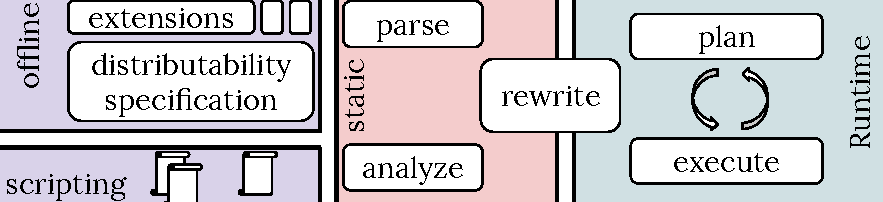
\includegraphics[width=0.49\textwidth]{\detokenize{./figs/dish_overview.pdf}}
%% \caption{
%%   \textbf{High-level schematic.}
%%   \sys leverages parallelizability analysis for built-in commands and any developer extensions (left) to automatically transform shell scripts (mid) and orchestrates their
%%   execution (right).
%% }
%% \vspace{-10pt}
%% \label{fig:schematic}
%% \end{figure}


%% Unfortunately, developing $p_1$'s distributed equivalent requires significant effort.
%% % For a user with many computers and larger inputs, 
%% % The scope of such rewrites, and therefore the cost of manual effort, can vary considerably.
%% For simple pipelines, fitting into restricted models of computation, this effort amounts to expressing the computation using the primitives provided by a big-data framework~\cite{mapreduce:08, ciel:11, spark:12, naiad:13} or domain-specific language~\cite{alvaro2011consistency,distal:13,meiklejohn2015lasp}---an unjustifiable cost for small, one-off pipelines that take a few minutes to compose (but are applied to large datasets).
%% More complex pipelines, such as the ones presented in later sections, would involve a full-fledged distributed programming language~\cite{erlang:96, lopes1997d, acute:05, mace:07, cloudhaskell:11, ScalaLoci:18}. %  or a distributed operating system---\eg Plan9's \ttt{rc} shell.
%% In both cases, manual rewriting is expensive and can introduce new bugs, cascading changes, and divergence from legacy functionality.
%% Could the generation and execution of $p_1$'s distributed version be fully and correctly automated?

%% To answer this question we develop \sys, a shell variant that transforms traditional \unix pipelines into their distributed equivalents, enabling \emph{distribution-oblivious programming}.
%% The key insight behind \sys is that a large part of the shell language can be encoded in a distributed dataflow graph model, providing structure to distribute computations.
%% %% \kk{Replaced that: the language of the Unix shell already encodes stream processing, providing most of the information required to distribute a computation. }
%% % FIXME \kk{I am not sure whether stream processing provides information for distributing a computation on its own. Maybe we can say that the shell exposes operator level parallelism, and that this is the first step to distributing a computation}.
%% \sys builds on this insight with a careful study of the parallelizability properties of shell primitives and commands, a definition of a dataflow graph model that is suitable for the shell, a set of parallelization optimizations that preserve the behaviour of the graph, and a late-bound command-prefixing scheme for deferring scheduling decisions to the distributed planner (\ie when runtime information is available).
%% A \sys-enabled $p_1$ will run \ttt{tr}s on parallel streams,
%%   use a mostly-parallel tree of \ttt{sort}s,
%%   run \ttt{uniq} mostly in parallel,
%%   execute \ttt{head} in one of the streams,
%%   and (trivially) merge streams in \ttt{out}.

%% % Developers of commands
%% % Developers of pipelines
%% % Language unifies both---no need for `-t` `-p`
%% % POSIX:
%%   % https://pubs.opengroup.org/onlinepubs/009695399/utilities/xcu_chap02.html

%% The combination of automated transformations for program distribution with the ability to maintain correct non-distributed semantics results in several benefits.
%% % \sys converts legacy shell pipelines into their distributed equivalents fully automatically, offering $100\times$ improvements in performance without a single line of additional code or annotation.
%% First, shell users composing pipelines (or simply running legacy pipelines on massive datasets) can see scalability benefits without any manual effort---no need for \ttt{qsub}~\cite{gentzsch2001sun}, \textsc{SLURM}~\cite{yoo2003slurm}, calls to \textsc{GNU} \ttt{parallel}~\cite{Tange2011a}, or any manual rewriting~\cite{mapreduce:08, ciel:11, spark:12}.
%% Second, developers of new shell commands can use a lightweight domain-specific language to express their parallelizability properties rather than ad-hoc, command-specific flags such as {\tt -t},  {\tt NUM\_THREADS}, \ttt{-t}, \ttt{-p} \etc
%% Most importantly, \sys provides an architectural lesson for system designers---namely, that large-scale efforts in the distributed- and operating-system literature to provide a \unix-like distributed equivalent~\cite{ousterhout1988sprite, mullender1990amoeba, pike1990plan9, barak1998mosix} would have been simplified by a thin (but sophisticated) rewriting shim like the one \sys provides.
%% % Nice critique on parallel: https://bugs.debian.org/cgi-bin/bugreport.cgi?bug=597050#75

%% % % Make Unix benefits explicit?
%% % Indeed, the primary reason behind $p_1$'s succinctness is that the pipeline is a domain-specific language for describing operations over streams.
%% % Key elements of \unix are the ability to compose programs written in different languages, the abstraction of a file system as a set of resident streams, a small but extensible library of commands, and the ability to resolve names within a global context.
%% % Under the hood, the \unix kernel buffers results, synchronizes processing stages, and generally orchestrates the computation.

%% The paper is structured as follows.
%% It starts by introducing the necessary background on shell scripting and overviewing \sys~\sx{bg}.
%% Sections \ref{parallelizability}--\ref{impl} highlight key
%% contributions:
%% \begin{itemize}

%%   \item
%%   \S\ref{parallelizability} studies several parallelizability classes and introduces the parallelizability characterization language.

%%   \item
%%   \S\ref{ir} presents a dataflow graph model for encoding shell pipelines, and a set of parallelization transformations that preserve the semantics of the sequential program.

%%   \item
%%     \S\ref{impl} describes the \sys implementation and addresses
%%     several challenges related to the translation and optimization of
%%     shell programs.
%%     %% details other concerns, such as distributed state management and extensibility. 
%% \end{itemize}

%% \noindent
%% \sys's evaluation~\sx{eval} shows significant speedups (4--10$\times$) for parallel execution using a combination of real pipelines. %micro-bench\-marks %---popular shell one-liners that highlight certain features---and a multi-line macro-benchmark---a popular weather analysis script.
%% After a comparison with related prior work~\sx{related}, the paper closes with a discussion of limitations and possible future directions~\sx{discussion}.
%% % \bigskip
%% % \begin{quote}
%% % \footnotesize
%% Additional material, in anonymized form, is available at
%% \href{https://git.io/Je6Nk}{https://git.io/Je6Nk}.
%% % \end{quote}

%% % \begin{figure*}[t]
%% % \centering
%% % 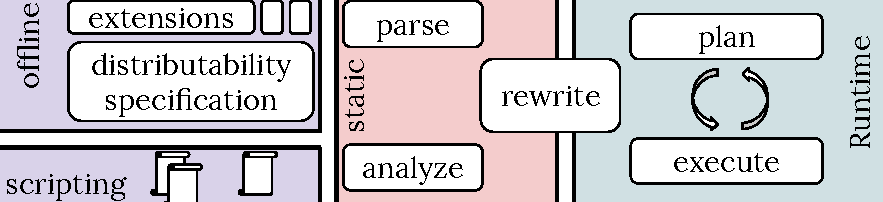
\includegraphics[width=0.49\textwidth]{\detokenize{./figs/dish_overview.pdf}}
%% % \caption{
%% %   \textbf{Applying \sys to $p_1$.}
%% % }
%% % \label{fig:example}
%% % \end{figure*}
%% % 

\section{Background and Overview}
\label{bg}

This section first reviews shell scripting through a small example~\sx{bg:pipelines}, which it then uses to present an overview of \sys's design and implementation~\sx{bg:overview}.

\subsection{Running Example: Weather Analysis}
\label{bg:pipelines}

\begin{figure}[t]
\centering
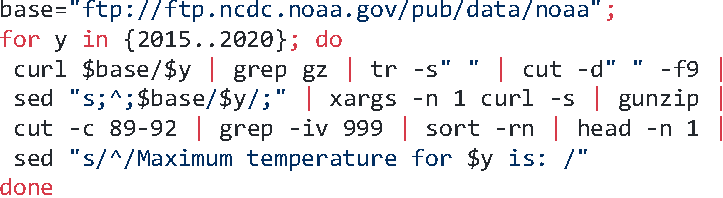
\includegraphics[width=0.49\textwidth]{\detokenize{./figs/dish_example.pdf}}
\caption{
  \textbf{Calculating maximum temperatures per year.}
  The script downloads daily temperatures recorded across the U.S. for the years 1920--2020 and extracts the maximum for every year.
}
\vspace{-15pt}
\label{fig:example}
\end{figure}

% In the ongoing debate on climate change,
Suppose a \todo{environmental scientist/engineer}    % looking for a non-CS expert---journalist might be too low
  wants to get a quick sense of the changes in maximum temperature over the past century.
As the National Oceanic and Atmospheric Administration (NOAA) has made historic temperature data publicly available~\cite{noaa}, 
  answering this question is only a matter of a simple data-processing pipeline.

The shell script in Fig.~\ref{fig:example} starts by pulling the yearly index files and filtering out URLs that are not part of the compressed dataset.
It then downloads and decompresses each file in the remaining set, extracts the values that indicate the temperature, and filters out bogus inputs marked as \ttt{999}.
It then calculates the maximum yearly temperature by sorting the values and picking the top element.
Finally, it matches each maximum value with the appropriate year in order to print the result.
% 
The effort required to write this pipeline is astonishingly low:\footnote{
  Some effort is required to understand NCDC's weather format, but this is true for any program processing this dataset.
}
  its data-processing core amounts to 12 stages and, when expressed as a single line, only 165 characters long.
To enable such a succinct program composition, \unix incorporates several features.

\heading{\unix Features}
Composition in \unix is primarily achieved through pipes (\ttt{|}), a
construct that allows for task-parallel execution of two commands by
connecting them with a character stream.
%% An important \unix feature are pipes (\ttt{|}), introducing
%% task-parallel program composition over character streams.
These streams are contiguous character lines separated by newline character (\textsc{NL}), which delineate individual stream elements.
For example, the first \ttt{grep} is given lines that contain file identifiers, of which it only outputs lines that contain \ttt{gz}, which are in turn consumed by \ttt{tr}.
% As part of this interface, each command has access to (any combination of) three \emph{standard} streams---input, output, and error.
A special end-of-file (\textsc{EOF}) condition marks the end of a stream.

Another important feature is synchronization, as different pipeline stages process data concurrently and possibly at different rates.
For example, the second \ttt{curl} produces output at a significantly slower pace than the \ttt{grep} commands before and after it.
The \unix kernel facilitates scheduling, communication, and synchronization behind the scenes.

Command flags, used pervasively in \unix, are configuration options that the command's developer has decided to expose to its users, to give command users significant freedom in their execution.
For example, by omitting  \ttt{sort}'s \ttt{r} flag that enables reverse sorting, the user can easily get the minimum temperature.
The shell does not have any visibility into these flags; 
  after it expands special characters such as \ttt{\textasciitilde{}} and \ttt{*}, it leaves parsing and evaluation entirely up to commands.

Finally, \unix provides an environment in which commands written in any language can be composed.
Many of the commands used in practice come built into the system---\eg commands defined by the POSIX standard or ones part of the GNU Coreutils---whereas others are available as add-ons.
The fact that commands are developed in a variety of languages---including shell scripts---provides users with a significant flexibility.
For example, one could replace the call to \ttt{sort} and \ttt{head} with one to \ttt{./avg.py} to get an average or a standard deviation rather than a maximum.
The pipeline would still work, as long \ttt{./avg.py} conforms to the interface outlined earlier.
% Shell scripting allows incremental development through refinement

% the input stream (stdin), the output stream (stdout), and the generating errors or diagnostics to the standard error stream (stderr)
% generating errors or diagnostics to the standard 
% Leveraging this interface, pipelines chain together commands by their standard streams, such that the output stream of one command (stdout) is passed directly as input (stdin) to the next one.
% \smallskip


% ---available publicly online via NCDC's NOAA~\cite{}---to obtain the maximum temperature per year.

\heading{Parallelization Challenges}
While these features aid developer economy through powerful program composition, they complicate shell script parallelization which even for simple scripts such as the one in Fig.~\ref{fig:example} face several challenges.
% \footnote{
%   Alternatives for automated parallelization were outlined in the introduction~\sx{intro} and are surveyed in the related work section~\sx{related}.
% }

One obvious challenge is due to the language of the shell, which has been developed through a long history of additions.
Different parts of a script, exploiting different language constructs, are amenable to different levels of parallelization---if at all.
% Some constructs, such as the parallel composition operator \ttt{\&} ; many others such as the sequential composition operator (\ttt{;}) are clearly sequential; yet others, such as the loop constructs are more difficult to categorize.
For example, Fig.~\ref{fig:example} assignment to \ttt{base}, connected with the rest of the script by the sequential composition operator (\ttt{;}), cannot be interleaved with the rest of the script.

Another challenge is due to the multitude of available commands;
  each command that is part of a script may require very different treatment.
For example, \ttt{grep} can proceed in parallel on each stream without any coordination, \ttt{head} requires light coordination, and \ttt{sort} requires significant coordination across streams.
Worse even, the same command may be used with different flags---\eg % \ttt{-d" " -f9} for the first
  Fig.~\ref{fig:example}'s \ttt{cut} is called twice with two different sets of flags\kk{I propose dropping the last sentence for this ``---making correct treatment even more difficult''}.
When a single flag can affect the functionality of a command in non-trivial ways, deciding how to parallelize becomes significantly more difficult.

Yet another challenge is that different phases operate on different output sizes thus allowing different parallelization widths.
Even if Fig.~\ref{fig:example}'s script was aiming on, say, only six years of data, the first \ttt{curl} would still output hundreds of lines for each year.
Naive, coarse-grained parallelization can miss such opportunities.

% \nv{Are these all the challenges we want to highlight?}


\kk{There are two ways to go here: either mention the challenges that a user would face to manually parallelize a script (that have already been mentioned in the introducion), or mention the challenges that automatic parallelization---this paper---has to address. I think that we should focus on the second.}

The first and greatest challenge is the gargantuan number of available
commands that can be used to construct a shell script. In contrast to
restricted programming frameworks that are amenable to parallelization
by supporting a few carefully designed operators (see MapReduce,
Spark, etc) shell scripts can contain commands that can have arbitrary
behaviours.  In order to parallelize such a script, each of command
requires special treatment as to not introduce non-determinism or
erroneous behaviours. For example, \ttt{grep} can be performed on
different partitions of its input in parallel without any
coordination, \ttt{head} requires light coordination, and \ttt{sort}
requires significant coordination.  To make matters worse, the same
command may be used with different flags---\eg % \ttt{-d" " -f9} for
the first Fig.~\ref{fig:example}'s \ttt{cut} is called twice with two
different sets of flags---that could potentially alter its behaviour,
making correct treatment even more difficult. A good solution should
handle several commands but should also be extensible, in the sense
that newly added or modified commands don't require modifications in
the solution itself. \kk{The solution to this challenge is already written in the third paragraph of the design overview.}

Another issue is that all commands are black boxes. Therefore it is
impossible to perform any kind of analysis on the code of the command
to identify possible parallelization. Therefore a good solution should
parallelize in a coarse-enough granularity that doesn't require
opening up commands.

Finally, shell scripts contain several constructs that enforce sequential execution. For example, Fig.~\ref{fig:example} assignment to \ttt{base}, connected with the rest of the script by the sequential composition operator (\ttt{;}), has to be completed before the rest of the script starts executing. \kk{The solution is
  written in the fourth paragraph of the design solution.}


\begin{figure}[t]
\centering
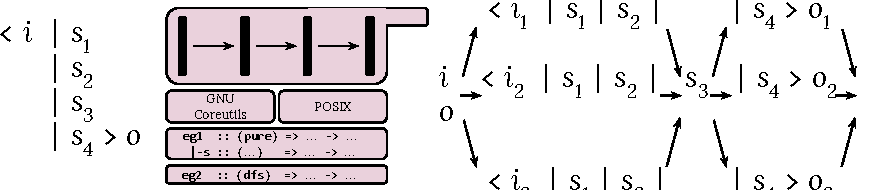
\includegraphics[width=0.49\textwidth]{\detokenize{./figs/dish_schematic.pdf}}
\caption{
  \textbf{\sys transformation overview.}
  Given a shell pipeline, \sys leverages command parallelizability to identify
  high-parallelizability stages, rewrite them, and orchestrate their execution.
}
\vspace{-15pt}
\label{fig:overview}
\end{figure}


% \heading{Generation}
% Expansion---the key is that expansion and evaluation are handled by the shell at an earlier stage 
% The most powerful---and interesting, for \ttt{dish}---type of expansion is subshell expansion, that allows replacing entire input streams 

\subsection{\sys Design Overview}
\label{bg:overview}

At a high level, \sys takes as input a POSIX shell script like the one in Fig.~\ref{fig:example} and outputs a new POSIX shell script.
The new script may incorporate parallelism, and is handed off to the user's original shell interpreter---\eg \ttt{bash} or \ttt{zsh}---for execution.
To \todo{discover and enable/expose and exploit} data-parallelism in a given shell script,
%% parallel execution,
\sys analyzes individual program fragments, addressing the challenges mentioned earlier.

\sys first needs to understand the POSIX constructs used to compose larger programs, indicating indicate different levels of candidacy for pararllelization.
To achieve this, \sys breaks POSIX constructs into a few broad classes:
 (i) the parallel-composition operator (\ttt{\&}) exposes task parallelism,
 (ii) special commands such as \ttt{xargs} and \ttt{tee} expose data parallelism,
 (iii) the pipe operator (\ttt{|}) is a candidate for both task and data parallelism, and
 (iv)  other composition operators such as \ttt{\&\&}, \ttt{||}, and \ttt{;} are barrier candidates.

Second, \sys needs to understand the parallelization characteristics of individual commands used to compose larger programs---a two-fold challenge.
To understand standard commands available in any shell, \sys groups POSIX and GNU commands into a small but clear set of well-understood parallelizability classes;
  these commands are already useful-enough to allow the composition of useful shell programs operating in practice.
To understanding the characteristics of commands that fall outside the built-in set, allowing new commands to leverage \sys's power, \sys leverages this study to define an annotation language for describing a command's key properties with respect to its parallelizability.
Such light annotations \kk{have to be written once per command (and not once per script) and} are aimed towards command developers (rather than users), who can quickly and easily capture the properties of the commands they are developing.
% We haven't introduced the notion of flags
% A command developer can only annotate the default behavior;
%   if a new flag is added a few years later, and if that flag alters the command's class, only then a new annotation is needed.

% Given a pipeline of commands and their parallelizability characteristics, \sys's next challenge is 
% \sys achieves this through a series of rewriting passes that perform dataflow analysis to identify distributable regions.
% It converts the AST to a dataflow graph, and iteratively performs graph transformations that expose data parallelism as task parallelism, while preserving the pipeline's correctness.

Provided information about the shell constructs and individual commands and their flags, \sys needs to analyze the given script and identify program fragments that are candidates for parallelization.
To achieve this, it converts sections of the script that are amenable to parallelization into a data-flow graph (DFG) representation.
% Second, \sys defines a dataflow graph model that is suitable for the semantics of the POSIX shell and proposes a set of parallelization optimizations that preserve the behavior of the dataflow graph.
This is a flexible representation that enables a series of local transformations that expose data-parallelism, converting the graph into its parallel equivalent.
%% , in which DFGs indicate the parallelizable regions.
Further transformations compile the DFG back to a parallel script that uses POSIX shell constructs to guide parallelism explicitly---while aiming at preserving the semantics of the sequential program.

Finally, \sys needs to provide correct, high-performance combiners for certain classes commands, and be proactive about (addressing) several practical challenges related to quirks of the \unix environment.
In terms of combiners, \sys offers a set of linkable components for stream splitting and merging;
  these commands live in the \ttt{PATH} and are addressable by name, which means they can be used like (and by) any other commands.
Practical challenges---related to task parallelism, deadlock prevention, and runtime performance---are addressed through a series of constructs that \sys provides.

Returning to the script of Fig.~\ref{fig:example}...\nv{I think we should show fragments of the resulting script}

The next few sections (\S\ref{parallelizability}--\ref{impl}) discuss the details.
% They also outline other, less obvious challenges---such as the synchronization of environment variables, distributed file operation, \etc.


\section{Parallelizability Classes}
\label{parallelizability}

To have any hope of parallelizing scripts, \sys first needs to understand the parallelization characteristics of the commands they contain.
As mentioned before \sys focuses on parallelizing data-parallel
commands, i.e. commands that can process their input in parallel, and
encodes their characteristics by assigning them to
\emph{parallelizability classes}.
%% This information is encoded in a command's \emph{parallelizability class}.
Intuitively, a parallelizability class represents the level of synchronization required by copies of a command that execute in parallel.
It focuses on capturing characteristics that are important for a command's parallel execution, rather than the command's full observable behavior.
\sys leans towards having a few coarse classes rather than many detailed ones---among other reasons, to simplify their understanding and use by command developers.
% Make the connections that this is like a type, that doesn't capture everything, but is good-enough

This section starts by defining these classes, along with a parallelizability study of the commands in {\sc POSIX} and GNU Coreutils~\sx{cmd}.
Building on this study, it develops a lightweight annotation language that enables command classification by its developers~\sx{ext}.
\sys in turn uses this language to annotate POSIX and GNU commands and generate their wrappers, as presented in later sections.

\subsection{Parallelizability of Standard Libraries}
\label{cmd}

\kk{Mention that commands change classes depending on their arguments and that we only write here (and in the table) the class of commands with no flags. Then the discussion about flags in the language part makes sense.}

% nv TODO: this is a hierarchy
Broadly, shell commands can be split into four major classes (summarized in Tab.~\ref{tab:classes}) with respect to their parallelization characteristics, depending on what kind of state they need when processing their input.
%% how they interact with state.
These classes are ordered in ascending difficulty of parallelization:
  later classes require more effort.
In this order, some classes can be thought as subsets of the next---\eg all stateless commands are pure---meaning that the synchronization mechanisms required for any superclass would work with its subclass (without seeing any performance improvements).

\begin{table}[t]
\center
\footnotesize
\setlength\tabcolsep{3pt}
\caption{
  \footnotesize{
    \textbf{Parallelizability Classes}.
    Broadly, \unix commands can be broken down into to \todo{four} classes according to their parallelizability properties.
  }
}
\begin{tabular*}{\columnwidth}{l @{\extracolsep{\fill}} llll}
\toprule
Class                    &  Key    & Examples                                    & Coreutils              & POSIX       \\
\midrule
Stateless                & ~\tsta  & \tti{tr},   \tti{cat},    \tti{grep}        &  22 (21.1\%)           & 22 (21.1\%)          \\  % 22
Parallelizable Pure      & ~\tpur  & \tti{sort}, \tti{wc},     \tti{uniq}        &  \todo{21 (20.1\%)}    & 21 (20.1\%)          \\  % 21
Non-parallelizable Pure  & ~\tnpu  & \tti{sha1sum}                               &  \todo{27 (25.9\%)}    & 27 (25.9\%)          \\  % 27
Side-effectful           & ~\tsid  & \tti{env},  \tti{cp}, \tti{whoami}          &  57 (58.8\%)           & 57 (58.8\%)            \\  % 25
% Irreversible     & ~\tirr  & \tti{exit}, \tti{lpr},    \tti{reboot}      &  5  (0.4\%)     & 5  (0.4\%)           \\  % 5
% \midrule
% Shell PL Constructs             &                         &                  \\
% \etc                            &                         &                  \\
\bottomrule
\end{tabular*}
\label{tab:classes}
\end{table}


% \heading{Preliminaries}
% \heading{POSIX, GNU Core-utils, and beyond}

\heading{Stateless Commands}
The first class, \sta, contains commands that operate on individual \todo{lines/elements}~\footnote{\todo{the choice of line as the data-quantum is deliberate, since they strike a nice balance between very coarse grained separation (files) and very fine-grained ones (individual characters). We might need to mention that in the introduction of 3.1}} of their input, without maintaining state across invocations.
These are commands that can be expressed as a purely functional $map$ or $filter$---\eg \ttt{grep} filters out individual lines and \ttt{basename} removes a path prefix from a string.
Stateless commands may produce multiple elements---\eg \ttt{tr} may insert {\sc NL} tokens---but when they receive empty input they return empty output.
Workloads that use only stateless commands are trivial to parallelize:
  they do not require any synchronization to maintain correctness, nor caution about where to split inputs.
 % map :: (a -> b) -> [a] -> [b]

\kk{Proposed insertion: The choice of where how to separate data elements would change the allocation of commands in parallelization classes---} Many of these commands (about 1/3 of \sta) are stateless \emph{within} a stream element---\eg\ttt{tr} transliterates characters within a line, one at a time---enabling further parallelization by splitting individual lines.
This feature may seem of limited use, as these commands are computationally inexpensive, precisely due to their narrow focus.
However, it turns to be  useful for cases with very large stream elements (long lines) such the \ttt{.fastq} format used in bioinformatics pipelines.  % TODO pointer to 6.3


\heading{Parallelizable Pure Commands}
The second class, \pur, contains commands that respect functional purity---\ie same outputs for same inputs---but maintain internal state across their entire pass.
The details of this state and its propagation during element processing affect their parallelizability characteristics.
Some commands are easy to parallelize, because they maintain trivial state and are commutative---\eg \ttt{wc} simply maintains a counter.
Other commands such as \ttt{sort}, maintain more complex invariants that have to be taken into account when merging partial results.

\begin{figure}[t]
\centering

\includegraphics[width=0.20\textwidth]{\detokenize{./figs/dish_classes.pdf}}
\caption{
  \textbf{Hierarchy of parallelizability classes.}
  Parallelizability classes form a hierarchy from the easiest to parallelize (left) to the most difficult (right).
  \nv{The figure is incorrect---it's actually a lattice.}
}
\vspace{-15pt}
\label{fig:example}
\end{figure}

Often these commands do not operate in an online fashion, but need to block until the end of a stream.
A typical example of this is \ttt{sort}, which cannot start emitting results before the last input element has been consumed.
\todo{Such constraints affect task parallelism, but not data parallelism}:
  \ttt{sort} can be parallelized significantly using divide-and-conquer techniques---\ie by encoding it as a group of (parallel) $map$ functions followed by a $fold$ that merges the results.

\kk{Maybe show an example of map-fold for sort or wc}

\heading{Non-parallelizable Pure Commands}
The third class, \npu, contains commands that, while purely functional, cannot be parallelized.
This is because their internal state depends on prior state in the same pass in non-trivial ways. % should we say something about state machines?
For example, hashing commands such as \ttt{sha1sum} maintain complex state that has to be updated sequentially.
If parallelized on a single input, each \todo{stage} would need to wait on the results of all the previous stage foregoing any parallelism benefits.

It is worth noting that while these commands are not parallelizable for a single input, they are still parallelizable across different inputs.
For example, a web crawler involving hash generation for comparing individual pages would allow \ttt{sha1sum} to proceed in parallel for different pages.

\heading{Side-effectful Commands}
The last class, \sid, are commands that have side-effects across the system---for example, updating environment variables, interacting with the filesystem, and accessing the network. \kk{Or commands that do not produce output consuming lines of their input---thus not being amenable to data-parallelism.}
Such commands are not parallelizable without finer-grained concurrency control mechanisms that can detect side-effects across the system.

This is the largest class because it includes commands related to the file-system---a central abstractions to the \unix design and philosophy~\cite{unix}.
In fact, \unix uses the file-system as a proxy to several file-unrelated operations such as access control and device driving. % is grafted upon the file-system.

\nv{
  A significant part of these commands (a ratio of 21:4) only \emph{read} values, and usually values that are never written by user code.
  For example, \ttt{date}, \ttt{uname}, and \ttt{finger} are all commands that interface with kernel- or hardware-generated information that is not writable by user-space scripts.
  Why aren't these parallelizable?
}

% \heading{Discussion}
% There are a few technical details about \sys's design decisions worth noting.

% %\nv{I took this out because it tooks about \sys's design/implementation that goes far afield}
% In terms of inputs, \sys supports commands with multiple input (resp. output) streams, by prepending (resp. appending) shell built-ins that merge input (resp. split output) streams~\sx{impl}.
% Thus, a command can be modelled as having one input and one output stream, a representation that is used throughout \sys including the extensibility DSL~\sx{ext}.
% 
% %\nv{I took this out because there are no more classes now}
% The focus for the rest paper will be commands in \sta and \pur.
% \sys currently treats other commands as non-distributable~\sx{discussion}.
% In future work, by building infrastructure to handle other classes, \sys will be able to (i) extract more parallelism and (ii) handle larger programs.
% Even with only these two classes, however, \sys distributes highly useful pipelines that are strictly more expressive than programs written in popular frameworks such as Hadoop~\cite{mapreduce:08} and Spark~\cite{spark:12}~\sx{eval}.

\subsection{Extensibility Annotations}
\label{ext}

\nv{Note command breadth/impossibility of our task.}
% https://nextbreakpoint.com/posts/article-compile-code-with-docker.html

%% Here is the type for \ttt{bwa}, a command that performs a Burrows-Wheeler transform over genomic data:
%% % ( bwa ) :: ( Pure )  => { In \/ File* } -> { Out /\ Err }    -- default case
%% %    | -h :: ( Sless ) => { Out }                              -- if needed
%% \begin{lstlisting}[language=sh, float=h, numbers=none, escapeinside={($}{$)}]
%% (bwa) :: (Pure) ($$\Rightarrow$$){In($$\lor$$)File*}($$\rightarrow$$){Out($$\land$$)Err}
%%   |-h :: (Sless)($$\Rightarrow$$){Out}                              
%% \end{lstlisting}

%% It states that the command defaults to the Pure class.
%% It's operation can be thought as a transformation from input streams to output streams.
%% It operates either on stdin or, if this doesn't exist, one or more files specified as arguments;
%% % TODO: check actual man page for how to specify files
%%   it writes to the output and error stream rather than a file.
%% The \ttt{-h} flag moves \ttt{bwa} into the Stateless class;
%%   its output is a constant function.

% % FIXME: \nv{TODO: remember to bubble up(me)}
% An important characteristic of the \unix shell is its
% language-agnostic extensibility~\sx{bg}.  Users composing pipelines
% are free to install custom commands available from various sources.
% Being general programs, commands are developed in a variety of
% languages and are extended over long periods of time.
% %% \kk{Text point: This restricts the space of solutions for
% %%   distribution of shell scripts}
% As a result, any static characterization of shell commands would bs
% unsatisfactory and would quickly become obsolete, supporting only a
% small subset of the commands needed in practice.  This poses a
% challenge to the developers of individual commands---how can they
% augment their commands to capture information critical to \sys without
% too much effort?
% %% \kk{Text point: The characteristics of a good solution}

To address the challenge of language-agnostic extensibility~\sx{bg}, \sys allows communicating several key details about command parallelizability through lightweight annotations.
These annotations can be used by both developers of new commands---which includes users developing their own scripts---as well as developers maintaining existing commands.
The latter can express additions or changes to the command's implmentation or interface, important as commands are maintained or extended over long periods of time.

\heading{Key Concerns}
\sys's annotations focused on three crucial concerns:
  (i) a command's parallelizability class,
  (ii) for commands that support multiple inputs, the characteristics of input consumption, and
  (iii) for commands with multiple flags (options), the handling of \todo{competing sets} of flags.
As the first concern was discussed extensively in the previous section, we now focus on the latter two.\footnote{
  \nv{Note to self: until now we have been talking only about parallelizability, and now we introduce two concerns that haven't been mentioned before.}
}

To be able to accurately construct the DFG representation, \sys needs to know certain information about a command's inputs and outputs.
There are couple of reasons for this.
One reason is due to \sys's DFG representation, which connects commands with each other;
  to perform this connection correctly \sys needs to know the outputs of a command to correctly connect them with the inputs of the next.
A second reason is due to ordering:
  as some commands consume their inputs in a certain order, this order needs to be maintained in the parallel version of the program.
For example, consider the parallel version of the expression \ttt{grep "foo" f1 f2}:

\begin{lstlisting}[language=sh, numbers=none]
  mkfifo t1 t2
  grep "foo" f1 > t1 &
  grep "foo" f2 > t2 &
  cat t1 t2
\end{lstlisting}

\noindent
This is correct only because \sys knows that \ttt{grep} in the sequential program reads from \ttt{f1} first and from \ttt{f2} second.

Command flags (options) are a particularly popular way to control a command's execution, directly affecting its parallelizability classification.
Commands are thus assigned a default parallelizability class, which is then refined by the set of flags the command uses.
For example, \ttt{cat} defaults to \sta, but with \ttt{-n} it jumps into \pur because it has to keep track of a counter and print it along with each line.

As parallelizability classes form a hierarchy from most parallelizable to least parallelizable~\sx{cmd}, a command is classified by the class of its least parallelizable flag.
For example, if a custom \ttt{trace-sort} command is invoked with flags \ttt{r}, \ttt{n}, and \ttt{k2} that are in \pur and a flag \ttt{d} that writes debugging output to a file, it ends up in \sta.

%% As simple examples, consider \ttt{cat} and \ttt{sort}.
%% By default \ttt{cat} is in \sta, but with \ttt{-n} it jumps into \pur because it has to keep track of a counter.
%% Conversely, \ttt{sort} defaults to \pur, but \ttt{with} \ttt{-h} it jumps into \sta because it generates a static stream regardless of other input.
% TODO: closure?

%% This is actually wrong. sort -h is not stateless since if called several times it produces the same output many times.
%% nv: the above does not mean it is not stateless; if apply `map` multiple times on an input I will get combined results.

%% Can be tweaked according to this:
%% https://tex.stackexchange.com/questions/24886/which-package-can-be-used-to-write-bnf-grammars


%% \heading{Command Inputs and Outputs}
%% A second concern captured by the AL is the order of inputs and outputs.
%% Commands generally read multiple input streams (and, at cases, write to multiple output streams).
%% The invariants between inputs and outputs must be maintained over the distributed execution of the program.
%% % but these maintain different invariants, enabling very different parallelizability characteristics.

%% Consider the command \ttt{comm} that takes as input two files and
%% performs a join operation. When invoked without any option, it
%% produces a three-column output. The first column contains lines that
%% are unique to the first file, the second column contains lines that are
%% unique to the second file, and the last column contains lines that
%% exist in both files. In the general case \ttt{comm} is in \pur, since
%% it needs to wait until it reads both files completely before it can
%% output its results.

%% However, \ttt{comm} can also be invoked using some options that
%% suppress the output of any combination of columns. More precisely, the
%% option \ttt{-1} suppresses the first column of the output. Similarly,
%% \ttt{-2} and \ttt{-3} supress the second and third column. Using both
%% \ttt{-2} (or \ttt{-1}) and \ttt{-3}, the command jumps to \sta
%% regarding its first (resp. the second) file argument.

% \ttt{comm} is in \pur, but with \ttt{/input1} it jumps into \sta---as it is now partially evaluated, it becomes stateless with respect to the second argument.

\heading{Example Annotations}
A record contains a set of clauses, each one identified by a predicate on the commands options.
Each clause maps to an assignment for the command, indicating its class and the sequence of its inputs and outputs.
Annotations treat flag arguments differently from file arguments, by checking if they start with a \ttt{-}.
% \footnote{
%   Note that the single character \ttt{-} is not an option as it is most often used to designate that a command reads from its standard input.
%   \nv{
%     There are options of of the form --f "x; y", and BSD options do not take \ttt{-} (like \ttt{ps aux}).
%     I am also not sure how important this last sentence is, as it did not answer a question I had---I expected arguments to be anything: if soneome wants to put ``pizza'' the DSL should not disallow it.
%   }
% }
The grammar of the language for specifying annotations is shown in Appendix~\ref{alg}.

For example, consider \ttt{comm}---a command that performs a join-like operation on its two inputs to identify common elements.
When \ttt{comm} is invoked without any flags, it produces a three-column output:
  the first column contains lines that are unique to the first input, the second column contains lines that are unique to the second input, and the last column contains lines that exist in both inputs.
A user can invoke \ttt{comm} with any combination of flags \ttt{-1}, \ttt{-2}, or \ttt{-3} to suppress the corresponding output columns.
Its annotation record is shown below:
%
\begin{lstlisting}[language=sh, numbers=none]
comm {
  | -1 /\ -3 =>
    (stateless, [args[1]], [stdout])
  | -2 /\ -3 =>
    (stateless, [args[0]], [stdout])
  | _  =>
    (pure, [args[0], args[1]], [stdout])
}
\end{lstlisting}

\noindent
The first two clauses describe \ttt{comm} invocations with options \ttt{-1} (or \ttt{-2}) and \ttt{-3}.
In the first case, since the first and third columns are suppressed, \ttt{comm} can be considered in \sta by regarding its first file argument as a static ``configuration'' input;
  this input accompanies every replicated instance of the command executing in parallel.
The general case, which includes \ttt{comm} invocations without any options, is captured by the third clause.
There, \ttt{comm} is classified as \pur, since it needs to wait until it reads both files completely before it can output its results.
Its inputs are its first and second file arguments (\ie excluding any options), and its output is produced in \ttt{stdout}.

%%  This case is described in the third clause of the annotation
%% record, where \ttt{comm} is classified as \pur, since it needs to wait
%% until it reads both files completely before it can output its
%% results. Its inputs are its first and second arguments (excluding the
%% options), and its output is produced in \ttt{stdout}.

%% The first and second clauses describe the case when \ttt{comm} is
%% invoked with options \ttt{-1} (or \ttt{-2}) and \ttt{-3}. In this
%% case, since the first and third columns are suppressed, \ttt{comm} can
%% be considered \sta by regarding its first file argument a static
%% ``configuration'' input. \kk{Does this need more explanation?}

%% \kk{I
%%   think that the language definition should be in a technical report,
%%   and here we should only give intuition and the \ttt{comm} example}
%% is designed to classify commands into multiple categories given their
%% options.

%% It assumes that the arguments of a command can always be separated to
%% options and file arguments (checking if they start with a
%% \ttt{-}~\footnote{Note that the single character \ttt{-} is not an
%%   option as it is most often used to designate that a command reads
%%   from its standard input}). A file written in the DSL contains a
%% record containing a mapping from predicates to assignments for each
%% command. Predicates can be simple boolean formulas on the existence
%% and the value of any option. Each assignment contains the command
%% category, the sequence of its input sources, and its output
%% source. Inputs to commands are a sequence of file identifiers and its
%% standard input. Similarly, the output is either its standard output or
%% a file identifier. An example record for \ttt{comm} can be seen below:

%% \begin{lstlisting}[float=h, numbers=none]
%%   comm {
%%     | -1 and -3 =>
%%       (stateless, [args[1]], stdout)
%%     | -2 and -3 =>
%%       (stateless, [args[0]], stdout)
%%     | otherwise =>
%%       (pure, [args[0]], stdout)
%%   }
%% \end{lstlisting}

%% The semantics of the language is straightforward: given a command, the
%% interpreter collects its options and then returns the assignment of
%% the first predicate that is satisfied. The final predicate is always
%% satisfied. For example the following two invocations of \ttt{comm}
%% would be classified as follows:

%% \begin{lstlisting}[language=sh, float=h, numbers=none, escapeinside={($}{$)}]
%%  comm -13 f1 f2 # => (stateless, f2, stdout)
%%  comm f1 f2     # => (pure, f1, stdout)
%% \end{lstlisting}



\tr{\kk{We don't need to designate the stderror, because we assume that it
  is never the main output of a command and it will never be used by
  the input of another command in the pipeline. If someone indeed
  wants to do this, they can just use a redirect I think to get around
  it.}}


\tr{\kk{If we talk about the language it would be good to give some
  statistics about how many commands (out of the ones that we have
  classified) can be represented with one, two clauses etc. If we have
  a different solution (like python function that given a command and
  its arguments returns the category) then we could talk about how
  many lines of code it took to categorize all the commands that we
  did.}}


\tr{\kk{Note: Since a categorization language will probably not be
  complete (especially the one showing the input arguments) there
  should be a backup mechanism, when the language is not expressive
  enough, like a python function that categorizes the command, and
  returns its input argument if it is stateless.}}

\tr{\kk{(Maybe) We should have a crisp point about why we have this categorization
  language, and why don't we just allow someone to write a function in
  python for each command, that given the command and its arguments,
  returns whether the command category. Possible arguments include,
  the fact that this language is simpler to use, especially by non
  experts that just run some script but have installed some commands
  that are not ``supported''. Another possible argument is that we
  could be able to reason about the constructs of the categorization
  lagnauge, and that they will be easier to read and
  understand. Another argument is that since these categorizations
  should be shareable among users, it would be bad to execute
  arbitrary python code, so using this language, expressivity is
  limited. All of these arguments are a little bit weak though. Niko,
  what do you think?}}


\heading{Providing Combinators}
For most commands, the annotations are enough to allow parallelization: 
  commands either fall under \sta, having straightforward combiners, or fall under a subset of \pur that can be parallelized using divide-and-conquer techniques~\sx{cmd}.
Unfortunately, there are commands with less trivial tactics---after all, \unix commands are Turing-complete programs and failing to plan for this generality would inhibit \sys's usefulness.

To support the parallelization of arbitrary commands in \pur, \sys allows command developers to provide custom $map$ and $fold$ functions.
In line with \unix philosophy, these functions can be written in any language as long as they conform to a few invariants:
  (i) $map$ in \sta and $fold$ is in \pur,
  (ii) $map$ can consume (or extend) the output of the original command and  $fold$ can consume (and combine) the results of multiple $map$ invocations, and
  (iii) their composition produces the same output with the original command.
If these invariants are met, after DFG analysis~\sx{ir} \sys can replace occurrences of these commands with their $map$ and $fold$ equivalents, enabling their parallelization.

\sys defines the combiners for most of the POSIX and Coreutils commands in \pur, which operate as both \sys's standard library and exemplar for community attempts to tackle other commands.


\tr{\kk{I am not sure a general interface is so easy to design. It needs
  more though. It might be beneficial to just talk about sort and wc
  here and how we implemented them and nothing more. Or maybe this
  could then go to the implementation? Or maybe say that one can write
  a python function that given a node of the graph, transforms it into
  many. I am not sure what is best...}}


% As mentioned in parallelizability, pure commands can be broken down
% into different categories. We might be able to get ideas about this
% from this paper:
% \url{http://www.cs.toronto.edu/~azadeh/papers/pldi17-ex.pdf} and its
% continuation in PLDI 2019.
% FIXME: \nv{Cite this paper?}
\tr{Can we find a solution for the commands in coreutils?}


\section{Dataflow Graph Model}
\label{ir}

The core of \sys is a dataflow graph model that is expressive enough
to support a large subset of shell programs. A fundamental difference
with other dataflow graph models is that in \sys's model contains
information about the order in which a node reads its inputs. This
enables a set of graph transformations that expose data parallelism as
task parallelism. These transformations can then be applied in an
iterative way, optimizing the program to utilize available
computational resources.


%% The core of \sys is a dataflow graph model, inspired by the ones used
%% in popular distributed stream processing systems~\sx{related} \kk{Is
%%   this reference here necessary?}. The dataflow model can express a
%% large subset of Shell programs and inherently supports the data
%% parallelism found in shell pipelines by exposing it as task
%% parallelism. More preciely, we have developed a set of
%% parallelization-exposing optimizations represented as
%% semantics-preserving graph transformations. These transformations can
%% then be applied in an iterative way, optimizing the program to utilize
%% available computational resources.

%% In order to effectively apply optimizations and distribute a shell
%% script, \sys first translates it to a manipulable representation.

\subsection{Definitions}
\label{graph-components}

The two main shell abstractions are (i) files (or pipes, \emph{viz.}
correspondence between files and pipes in \S\ref{bg:pipelines}) that
contain data, and (ii) commands that communicate through these
files. Based on that, in \sys's graph model nodes represent commands
and edges represent files.

We first introduce basic notation that will be useful later on.  For a
set $D$, we write $D\kstar$ to denote the set of all finite words over
$D$. For words $x, y \in D\kstar$, we write $x \cdot y$ or $xy$ to
denote their concatenation. We write $\eps$ for the empty word. We say
that $x$ is a \emph{prefix} of $y$, and we write $x \leq y$, if there
is a word $z$ such that $y = xz$. The $\leq$ order is reflexive,
antisymmetric, and transitive (i.e. is a partial order) and is often
called the \emph{prefix order}.


\heading{Edges -- Files}

Edges in the dataflow graph represent files, the basic data
abstraction of the shell. They are used as communication channels
between nodes in the graph, and as the input or output of the whole
graph. Edges are represented as possibly unbounded streams of type
$D\kstar$. Edges can either refer to named files or FIFO pipes used
for interprocess communication. Edges that do not start from a node in
the graph represent the graph input; edges that do not point to a node
in the graph are its outputs.



%% \TODO{Show an example pipe and its graph}.

%% \begin{center}
%% \small
%% \begin{tikzpicture}[node distance=2.25cm, ->]
%% \node (S) {};
%% \node (A) [draw, right of=S, node distance=1.75cm] {node 1};
%% \node (B) [draw, right of=A] {node 2};
%% \node (C) [draw, right of=B] {node 3};
%% \node (E) [right of=C, node distance=1.75cm] {};
%% \path (S) edge node[above] {input} (A);
%% \path (A) edge node[above] {stream} (B);
%% \path (B) edge node[above] {stream} (C);
%% \path (C) edge node[above] {output} (E);
%% \end{tikzpicture}
%% \end{center}

%% \tr{On the other hand, some forms of data parallelism can be exposed
%%   when knowing the size of the input files. As mentioned in \ref{}
%%   some pure commands (such as cat -n) only need line information to
%%   become stateless, and knowing the size of a file could allow the
%%   system to split it in different chunks that can be processed
%%   independently. To account for that, edges that refer to an input
%%   resource contain the number of lines of the file that they refer
%%   to.}


\heading{Nodes -- Commands}

A node $f$ of the graph represents a function from a (possibly empty)
list of inputs
%% streams
to a list of outputs
%% streams
$f : [D\kstar] \to [D\kstar]$, where $D$ represents the basic data
type of a line of characters.
%% \km{Is the number of input/output
%%   streams variable? If $m$ is the number of input streams, is the
%%   number of output streams a function of $m$? If this the case, then
%%   it is not captured by this type. Maybe it would help to show a
%%   couple of example operators together with the types of their
%%   denotations. A graphical representation (as in
%%   Fig.~\ref{fig:parallelization-transformation} would also be nice.}
%% \kk{Is there a reason to restrict the number of outputs to be a
%%   function of the number of inputs? I think that we don't need such a
%%   restriction, therefore the above type should be fine.}
This representation captures \todo{the majority/all} of commands in
the \tsta, \tpur, \tnpu. Note that these functions should only produce
output in the form of files and not perform any other side effect,
such as sending signals.  We require that the function $f$ is monotone
w.r.t.\ a lifting of the prefix order for a sequence of inputs
%% \kk{Formalize
%%   this lifting if essential for later development}.
%% More formally, $\forall f, x, y, f(x) = y$, then for any $x'$, there
%% exists $y'$ such that $f(x.x') = y.y'$, where $.$ is standard
%% concatenation and will be omitted when obvious.
This captures the idea that a node cannot retract output that it has
already produced.

\heading{\todo{Streaming} Commands}

\todo{Streaming} commands consume their inputs sequentially and one
element at a time, with the possible exception of static input files,
and produce one output file. The quintessential example of
\todo{streaming} commands is \ttt{cat}, that consumes its inputs in
order, producing their concatenation as output. A more interesting
example is \ttt{comm -23 f1 f2}, which has \ttt{f2} as its static
input (it needs to read it completely before consuming anything from
\ttt{f1} and then consumes \ttt{f1} one element at a time. These
commands can be represented as functions of type $f : D\kstar \times
[D\kstar] \to D\kstar$, where the first argument represents the
concatenation of the inputs that are consumed one at a time and the
second argument represents the static inputs.
%% \km{Again, a graphical
%%   presentation of these operators would be useful. Maybe with a way to
%%   distinguish between between streaming inputs and static inputs? Btw,
%%   this distinction is not completely clear to me at this
%%   point. Clearly, not all programs that we can write are streaming
%%   (monotone).} \kk{Do you mean that there are shell scripts that are
%%   non monotone? That is true but we are assuming monotone nodes. Do I
%%   miss something?}
We focus on these commands because a large subset of \sta and \pur
commands fall in this category.

%% \kk{Do we want to get in more detail about requirements? Commands must
%%   be deterministic, they must not do any other side effect (sending
%%   signals, etc). These assumptions must be checked when the developer
%%   designates the categories. Commands are assumed to always terminate
%%   gracefully. \sys changes the termination behaviour of commands as a
%%   sequential command that would exit prematurely might not exit
%%   completely if parallelized.}

%% \kk{If we have time and space we could give an example of a script
%%   together with its dataflow graph to give more intuition about nodes
%%   and streaming commands.}


%% An example of a node with one input and one output stream is the
%% following command:

%% \begin{lstlisting}[language=sh, float=h, numbers=none, escapeinside={($}{$)}]
%%  grep ``foo''
%% \end{lstlisting}

%% \noindent
%% This command takes a stream of lines from its standard input and
%% returns a stream of lines on its standard output.

%% An important observation is that even though commands might read their
%% input from several input streams, the order in which they read is not
%% always arbitrary. An illustrative example is the command \ttt{cat},
%% which consumes its input one stream at a time:

%% \begin{lstlisting}[language=sh, float=h, numbers=none, escapeinside={($}{$)}]
%%  cat x - y
%% \end{lstlisting}

%% \noindent
%% In the example above, \ttt{cat} reads file \ttt{x} until it encounters
%% the EOF character, then reads from \ttt{stdin} until in encounters
%% EOF, and finally reads from \ttt{y}. Other commands that read their
%% inputs one file at a time include \ttt{grep} and \ttt{tr}. Knowing the
%% order in which a node consumes its input is necessary to enable
%% certain optimizations on the graph.

%% \kk{Some could read in sequence (like cat), some in lockstep (like
%%   zip), some read some files statically and the rest as streams (like
%%   comm), some read arbitrarily.}


%% \kk{I need to mention that there are nodes that we know more
%%   properties of. For example cat, tee, zip, etc... and these are
%%   handled specially because of their very important and special
%%   properties.}


%% \begin{figure*}
%% \centering
%% \begin{tikzpicture}[->, >=to, auto, node distance=1cm, semithick, transform shape, inner sep=2pt]
%% %
%% \small
%% %
%% \node (M1) {};
%% \node (M2) [draw, right of=M1, node distance=2cm] {Map};
%% \node (M3) [draw, right of=M2, node distance=3cm] {GroupBy(Reduce)};
%% \node (M4) [right of=M3, node distance=3cm] {};
%% %
%% \path (M1) edge node {input} (M2);
%% \path (M2) edge node {stream} (M3);
%% \path (M3) edge node {output} (M4);
%% \end{tikzpicture}
%% \end{figure*}

%% \begin{figure*}
%% \newcommand{\Split}{\text{Split}}
%% \newcommand{\Merge}{\text{Merge}}
%% \newcommand{\Map}{\text{Map}}
%% \newcommand{\GroupBy}{\text{GroupBy}}
%% \newcommand{\Reduce}{\text{Reduce}}
%% \centering
%% \begin{tikzpicture}[->, >=to, auto, node distance=0.6cm, semithick, transform shape, inner sep=1.75pt]
%% %
%% \footnotesize
%% %
%% \node (M1) {};
%% \node (M2) [draw, right of=M1, node distance=1.3cm] {$\Split$};
%% \node (M3) [right of=M2, node distance=1.5cm] {};
%% \node (M4) [right of=M3, node distance=2.5cm] {};
%% \node (M5) [draw, right of=M4, node distance=2.2cm] {$\Merge$};
%% \node (M6) [draw, right of=M5, node distance=3.8cm] {$\GroupBy(K_2,\Reduce)$};
%% \node (M7) [draw, right of=M6, node distance=3cm] {$\Merge_K$};
%% \node (M8) [right of=M7, node distance=2cm] {};
%% %
%% \node (T3) [draw, above of=M3] {$\Map$};
%% \node (T4) [draw, above of=M4] {$\Split_K$};
%% \node (T5) [draw, above of=M5] {$\Merge$};
%% \node (T6) [draw, above of=M6] {$\GroupBy(K_1,\Reduce)$};
%% %
%% \node (B3) [draw, below of=M3] {$\Map$};
%% \node (B4) [draw, below of=M4] {$\Split_K$};
%% \node (B5) [draw, below of=M5] {$\Merge$};
%% \node (B6) [draw, below of=M6] {$\GroupBy(K_3,\Reduce)$};
%% %
%% \path (M1) edge node {$A$} (M2);
%% \path (M2) edge[bend left=10] node {$A$} (T3);
%% \path (M2) edge[bend right=10] node[swap] {$A$} (B3);
%% \path (M5) edge node {$K_2 \times B$} (M6);
%% \path (M6) edge (M7);
%% \path (M7) edge node {$K \times B$} (M8);
%% %
%% \path (T3) edge node {$K \times B$} (T4);
%% \path (T4) edge (T5);
%% \path (T4) edge (M5);
%% \path (T4.330) edge[bend right=10] (B5.170);
%% \path (T5) edge node {$K_1 \times B$} (T6);
%% \path (T6) edge[bend left=10] node {$K_1 \times B$} (M7);
%% %
%% \path (B3) edge node {$K \times B$} (B4);
%% \path (B4) edge (B5);
%% \path (B4) edge (M5);
%% \path (B4.30) edge[bend left=10] (T5.190);
%% \path (B5) edge node {$K_3 \times B$} (B6);
%% \path (B6) edge[bend right=10] node[swap] {$K_3 \times B$} (M7);
%% %
%% \end{tikzpicture}
%% \caption{Distributed implementation of the map-reduce pipeline $\Map \gg \GroupBy(K,\Reduce)$.}
%% \label{fig:mapReduce}
%% \end{figure*}


\subsection{Graph Transformations}
\label{ir:transformations}

%% \kk{Move this assumption in the transformation: Nodes may read from
%%   more files than just the files of their input stream (resp. write to
%%   more files than their output stream).  However, these files are
%%   static (\eg used for configuration or logging) and do not represent
%%   streams of data, and therefore are not considered part of the
%%   dataflow graph.  For now, we assume that these static files can only
%%   be accessed by one node, thus ensuring that they do not interfere
%%   with the distributed implementation.
%% %% Because of the assumption in section Front End \ref{}, that each file
%% %% exists only once in the dataflow graph, we can safely assume that
%% %% reading and writing to these static files does not interfere with the
%% %% distributed implementation, and doesn't alter the behaviour of the
%% %% program.
%% }

We have defined a set of semantics-preserving graph transformations
that act as parallelization-exposing optimizations. Both the domain
and range of these transformations is a graph in our dataflow model
and therefore they can be composed arbitrarily and in any order.
%% Having a dataflow graph representation allows us to define
%% parallelization optimizations as graph transformations.
Before describing the different types of optimizations, we formalize
the intuition about stateless and pure commands that was described
earlier~\sx{cmd}.

%% We focus on \todo{streaming} commands (as defined in
%% \cref{graph-components}) that constitute a large subset of shell
%% commands.

%% \nv{TODOs
%%   (i) highlight earlier the antithesis between the formalisms in this section and the informalities of the previous (me)
%% }

%% \kk{Maybe
%%   have an argument here that we show in the evaluation that handling
%%   these commands is adequate for a big variety of data processing
%%   scripts (and most stateless and pure commands), from several
%%   microbenchmarks to some large-realistic macrobenchmarks.}.

\heading{Stateless and Parallelizable Pure Commands}

As mentioned in \Cref{cmd}, stateless commands such as \ttt{tr}
operate independently on individual elements of the stream
(characters, lines, or files) without maintaining any state. In this
work, we consider lines as the data quantum, so only commands that are
stateless regarding lines (or any finer granularity such as
characters) are considered stateless. Formally, a
\todo{streaming} command $f$ is stateless if it commutes with
the operation of concatenation, \ie it is a semigroup homomorphism:
%% with respect to concatenation \km{It commutes with the operation of concatenation. This is the definition of (semigroup) homomorphism. I am not sure that linearity is an appropriate term.}
%% , \ie satisfying the following equation:

\[
\forall x, x', s, f(x \cdot x', s) = f(x, s) \cdot f(x', s)
\]

%% This is a nice characterization, which I think is true in most
%% settings. There is a caveat though: You can have stateless programs
%% that emit output when they start (before they consume the stream)
%% and/or when they consume the EOF symbol. In this case I am not sure
%% the equation above holds.

\noindent
This means that applying the command $f$ to a concatenation of two
inputs $x, x'$ produces the same output as applying $f$ to each input
$x, x'$ separately, and concatenating the outputs.

Similarly, some pure commands (such as \ttt{sort} and \ttt{wc}) can be
parallelized using divide-and-conquer techniques. More formally, these
pure commands $f$ can be implemented as a combination of functions map
$m$ and an associative fold $f'$, satisfying the following equation:

\[
\forall x, x', s, f(x \cdot x', s) = f'(m(x, s) \cdot m(x', s), s)
\]

\noindent
This means that we get the same output by applying $f$ to a
concatenation of two inputs $x, x'$, or by applying the fold function
$f'$ to the concatenation of the outputs produced by applying map $m$
to each of these inputs.
%% \km{We had also discussed here the case of
%%   operators that can be described as associative and commutative
%%   functions on the data (e.g., sum). In this case the parallelization
%%   has the flavor of data parallelism: one can split the input stream
%%   in an arbitrary way (e.g., randomly or using some other
%%   load-balancing scheme) and merge the outputs. For the more broad
%%   class of associative operations (e.g., sort), the formulation of
%%   this paragraph makes perfect sense. I just want to mention that this
%%   feels a lot more like \textbf{batching} than map-reduce-like data
%%   parallelization.} \kk{Thanks, I think you are right. Batching is a
%%   better name for it. In the end we didn't handle
%%   commutative-associative function (that are more like map-reduce) and
%%   so we changes the name to map-fold to not imply commutativity.}

\heading{Parallelization Transformations}
%
Based on these equations, we can define a \emph{node parallelization
  transformation} on a stateless node $v$ that is preceded by a
\ttt{cat} with $n$ input streams and is followed by a node $v'$. The
transformation replaces $v$ with $n$ new nodes, routing each of the
$n$ input streams to one of them, and commutes the \ttt{cat} node
after them to concatenate their outputs and transfer them to
$v'$. Since each incoming edge represents a stream of data $x_i :
D^*$, and the only behaviour of a dataflow graph is its output, this
optimization $v(x_1 \cdot x_2 \cdots x_n, s) \Rightarrow v(x_1, s)
\cdot v(x_2, s) \cdots v(x_n, s)$ can be shown to preserve the
behavior of the graph. Furthermore, it can be straightforwardly
extended to pure commands that can be implemented by a map-fold pair
$(m, r)$ as $ v(x_1 \cdot x_2 \cdots x_n, s) \Rightarrow r(m(x_1, s)
\cdot m(x_2, s) \cdots m(x_n, s), s)$. \todo{A visual representation
  of this transformation can be seen in}
\Cref{fig:parallelization-transformation}.

\begin{figure}[t]
\centering
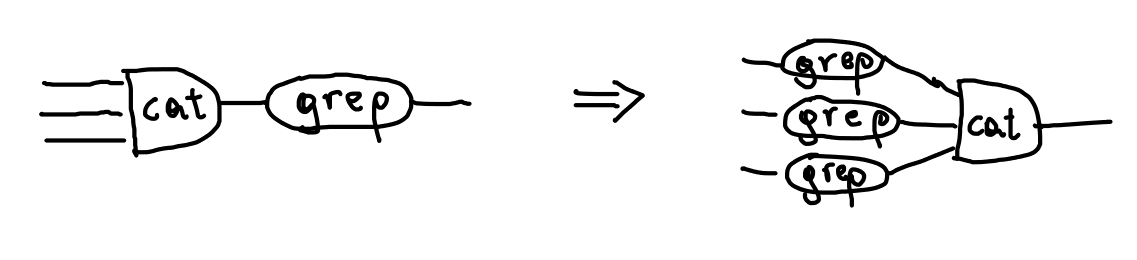
\includegraphics[width=\columnwidth]{\detokenize{./figs/transformation-sketch.png}}
\caption{
  \textbf{Stateless parallelization transformation.}
  The \texttt{cat} node is commuted with the stateless node
  to utilize available data parallelism.
  \TODO{Correct this diagram to show the cat node before
    the node and then the cat node after the stateless
    command after the optimization. Cat node should be
    different than a circle. Maybe like an ``and'' node
    in binary circuits?}
}
\vspace{-10pt}
\label{fig:parallelization-transformation}
\end{figure}

\heading{Auxiliary Transformations}

In addition to the above, we also define a set of auxiliary
transformations that are shown in
\Cref{fig:auxiliary-transformations}.  The first two enable the
parallelization transformations by inserting \ttt{cat} nodes, either
by using them to concatenate many inputs of one command, or by first
adding a \ttt{split} node that splits the input in batches. The final
one inserts a relay that performs the identity transformation on its
input. Relay nodes can be useful for monitoring and debugging, as well
as for performance improvements, as we will see in \Cref{optimizer}.

\begin{figure}[t]
\centering
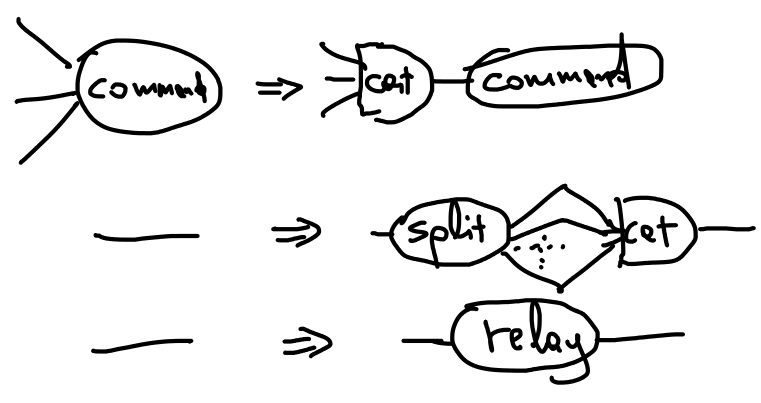
\includegraphics[width=\columnwidth]{\detokenize{./figs/auxiliary-transformations.png}}
\caption{
  \textbf{Auxiliary transformations.}
  \todo{Add all three of the auxiliary transformations.}
}
\vspace{-10pt}
\label{fig:auxiliary-transformations}
\end{figure}

%% \kk{Remember to mention the assumptions that need to hold for the
%%   graph transformations to be valid in the Command categories
%%   section. Commands must be deterministic, they must not do any other
%%   side effect (such as writing to other files, sending signals,
%%   etc). However, these assumptions must already be checked when the
%%   developer designates the categories. Commands are assumed to always
%%   terminate gracefully. \sys changes the termination behaviour of
%%   commands as a sequential command that would exit prematurely might
%%   not exit completely if parallelized.}

\tr{If there is time I can work out a formal definition and a proof
  sketch why this transformation preserves the output of the dataflow
  graph.}

%% \begin{definition}
%% Given a dataflow graph $G = (V, E, O)$, where $V$ is a set of nodes
%% representing commands, $E$ is a set of edges representing files, and
%% $O$ is a function from $V \cup v_{out}$ to a total order of incoming
%% edges. $v_{out}$ represents a concatenation of all the outputs of the
%% dataflow graph. We represent the total order for a node $v$ as
%% $<_v$. Given a node a node $v$
%% with input edges $ie = \{ i_1 = (v_{i_1}, v, 1), i_2, ..., i_n =
%% (v_{i_n}, v, n) \}$ and output edge $o = (v, v_o, a)$, we define a
%% complete node split $s(v, G) = (V', E')$ where $V' = V - v \cup \{
%% v_1, ..., v_n \}$ and $E' = E - ie \cup \{(v_{i_1}, v_1, 1), ...,
%% (v_{i_n}, v_n, 1) \} - o \cup \{ (v_1, v_o\}$
%% \end{definition}

%% \begin{lemma}
%% tofill
%% \end{lemma}


\section{Implementation}
\label{impl}

This section describes challenges related to the implementation of
\sys. It starts by describing how the \sys front-end translates a
shell script to the dataflow graph model defined in \S\ref{ir}, by
applying transformation on parallelizable regions~\sx{front-end}.  It
closes with the \sys runtime\todo{/backend} and the technical
challenges that were addressed to achieve performance
benefits~\sx{optimizer}.

\subsection{Front End}
\label{front-end}

As mentioned in \Cref{ir}, in order to optimize a shell script, \sys
translates it to a dataflow graph.  However, there are several
components in shell programs that cannot be arbitrarily parallelized
without affecting the program behaviour---\eg commands connected with
a \ttt{\&\&} operator~\sx{bg}.
%% In addition, the shell's highly dynamic
%% nature compounds the challenge---\eg by not knowing what files does an
%% unexpanded command argument refer to.
To address this issue, we introduce the notion of parallelizable
program regions and a translation pass for converting them to dataflow
dataflow graphs.

%% \kk{Give examples of writing to environment variables, producing
%%   irreversible side effects, the ; and \&\& operators.}

%% To address the first issue, we introduce the notion of parallelizable
%% program regions and a translation pass for converting them to a
%% dataflow graph. To address the second issue, we limit dynamic
%% components by deferring translation as late as possible using a
%% wrapping scheme.

%% The translation pass identifies distributable regions and
%% translates each of them to a dataflow graph, provided the abstract
%% syntax tree (AST) of a shell script.  The AST is produced by
%% \ttt{LibDash}, a POSIX compliant parser~\cite{libdash}.

\heading{Parallelizable Regions}
%
%% \kk{The goal of this subsection is to explain that Dish does a safe
%%   but effective analysis to identify which parts of the scripts to
%%   parallelize.}
%
Parallelizable regions are program sub-expressions that can be
parallelized safely without altering the total program behaviour.
%% respect to their sequential execution.
The search for these regions can be guided by the structure of shells
programs, which inherently contains information about components that
can be executed independently and barriers that are natural points for
enforcing synchronization. Consider the following example:

\begin{lstlisting}[language=sh, float=h, numbers=none, escapeinside={($}{$)}]
  cat f1 f2 | grep "foo" > f3 && sort f3 
\end{lstlisting}
% # Replace sort with sth better

\noindent
The commands \ttt{cat f1 f2} and \ttt{grep "foo"} would execute as
independent processes in the standard shell, while \ttt{sort f3} would
wait for their completion before executing.  Both \ttt{cat f1 f2 |
  grep "foo" > f3} and \ttt{sort f3} are therefore parallelizable
regions, regions that cannot be extended beyond \ttt{\&\&}---even
better, they are maximal.

Intuitively, parallelizable regions correspond to sub-expressions of
the program that would be allowed to execute independently by
different processes in the POSIX standard~\cite{posix}. Larger
parallelizable regions can be composed from smaller ones using the
pipe operator \ttt{|} and the parallel composition operator \ttt{\&}.
Conversely, all other operators, such as the \ttt{;} sequential
composition operator, the \ttt{\&\&} logical operator represent
barrier constructs that do not allow parallelizable regions to
permeate through.

% \tr{I don't know whether I should mention the following: While these
%   control flow constructs can be parallelized and there has been
%   research on it, it is orthogonal to our work, and can be
%   incorporated as future work.}
% 
% \begin{lstlisting}[language=sh, float=h, numbers=none, escapeinside={($}{$)}]
%   (tr ... f1 > g1 && tr ... f2 >> g1) &
%   grep ``foo'' g1
% \end{lstlisting}
% 
% In the above example, while \ttt{tr ... f1 > g1}, \ttt{tr ... f2 >>
%   g1}, and \ttt{grep ``foo'' g1} are all in different dataflow graphs,
% the dataflow graph that corresponds to the whole program, has two
% nodes, \ttt{tr ... f1 > g1 \&\& tr ... f2 >> g1} and \ttt{grep ``foo''
%   g1}.
% 

\heading{Translation Pass}

%% \kk{It might be a good idea to change this subsection based on the new
%%   as-late-as-possible architecture where everything is wrapped and
%%   translated at the final moment. Ideally, this would become the main
%%   point of this subsection, as the translation algorithm is kind of
%%   redundant when having the distributable regions too.}

The \sys front-end performs a depth-first search pass on the AST of
the given shell program.  During this pass, it extends the
parallelizable regions from the bottom up, translating their
independent components to dataflow graph nodes until a barrier
construct is reached. All subtrees that are not translated to dataflow
graphs are kept as they are. The output of the translation pass is the
original AST where parallelizable regions have been replaced with
dataflow graphs and a call to \sys's runtime.

To identify possible opportunities for parallelism, the translation
pass extracts the parallelizability class of each command together
with its inputs and outputs. It achieves that by searching all
available PAL~\sx{ext} records for each command and resorts to
conservative defaults if a record for the command is not found. If the
command is \sta or parallelizable \pur, the translation pass initiates
a parallelizable region that is propagated up the tree.

%% Finally, whenever the algorithm encounters a command, it first
%% checks whether it is safe to parallelize it. A command is considered
%% safe for parallelization if (i) it belongs to the \sta or \pur parallelizability classes, and (ii) does not read from a read-once file (such as a pipe containing configuration data) as parallelization would break this. % why couldn't we replicate this?
%% If the command is safe, \sys creates a node containing that command  and adds it to a singleton dataflow graph.
%% If the command is unsafe, it is still added to the dataflow graph, but is not further parallelized by the optimizer.


%% A few illustrative cases of the analysis algorithm are shown in pseudocode below:

%% \begin{lstlisting}[language=python, float=h]
%%   def translate(node):
%%     ...
%%     elif(node.name == 'Pipe'):
%%       return pipe_graphs([translate(child)
%%         for child in node.children])
%%     elif(node.name == 'And'):
%%       node.children = [translate(child)
%%         for child in node.children]
%%       return node
%%     elif(node.name == 'Command'):
%%       if(not safe(node)):
%%         return make_ir_node(node, 'unsafe')
%%       else:
%%         return make_ir_node(node,
%%           find_category(node))
%%     ...
%% \end{lstlisting}

%% Whenever the algorithm encounters a distributable node, it recursively
%% translates its subcomponents.
%% It then merges them in a dataflow (sub-)graph, connecting the output of the first with the input of the second
%% % what first and second? we didn't say anything about first and second
%% Before the different dataflow graphs are connected, the
%% algorithm checks that at most one node in the graph writes at every
%% file, and that at most one node reads from a file that another node writes
%% to. This is important, in order to avoid inconsistent behaviour after
%% distributing nodes in the dataflow graph (\ie by introducing to
%% concurrent reads and writes to the same file when
%% parallelizing).

%% Whenever the algorithm encounters a barrier node,
%% it recursively translates its subcomponents, similarly to the distributable
%% case.
%% However, different from the distributable case, it does not merge them in a large dataflow graph.

%% Finally, whenever the algorithm encounters a command, it first
%% checks whether it is safe to parallelize it. A command is considered
%% safe for parallelization if (i) it belongs to the \sta or \pur parallelizability classes, and (ii) does not read from a read-once file (such as a pipe containing configuration data) as parallelization would break this. % why couldn't we replicate this?
%% If the command is safe, \sys creates a node containing that command  and adds it to a singleton dataflow graph.
%% If the command is unsafe, it is still added to the dataflow graph, but is not further parallelized by the optimizer.

An important consideration is that due to the highly dynamic nature of
the shell, there is information (such as the values of environment
variables) that are not known to \sys at the time of translation.
%% to the the safety properties that are mentioned above cannot be
%% soundly checked statically.
For safety purposes, \sys takes a conservative approach where it does
not parallelize nodes without complete information.  For example, the
translation pass cannot infer that an environment variable that is
given as an argument to a command is not a flag that changes its
parallelizability class,
%% two un-expand strings do not refer to the same file identifier,
and as a result does not parallelize this sub-expression.

\kk{Can we say anything more about the safety considerations? That (i)
  the translation pass ``checks'' that no nodes write/read or
  write/write to the same file (is that necessary?), that (ii) a
  command should not read from a read-once file. (is that necessary?)}

%% \kk{Ideally we would want to talk here about the as-late-as possible
%%   dish translation that allows us to be safe despite the Shell's
%%   dynamic nature. I think that this is a great point about the
%%   work. Maybe we should also focus on implementing it before the OSDI
%%   deadline.}

\subsection{Runtime/Back End}
\label{optimizer}

%% \kk{Maybe guide all of this by showing an example of an output shell
%%   script?}

After translating the parallelizable regions of the input script to
dataflow graphs and optimizing these graphs using the transformations
described in \Cref{ir:transformations}, \sys implements the graph by
translating it back to a shell script. In this section we describe how
\sys achieves that, and several technical challenges that it addresses.


%% Given a dataflow graph representing a shell program, the \sys
%% optimizer outputs an optimized dataflow graph in which data
%% parallelism opportunities have been exploited.  More concretely, the
%% optimizer starts by splitting input files in several chunks, given the
%% desirable output dataflow graph width. It then starts from the source
%% nodes of the graph, iteratively performing the graph transformations
%% that were described in \Cref{ir:transformations}.
%% %% If the incoming edges of the node are less than the desirable graph
%% %% width, it performs edge splits, and then it performs maximal node
%% %% splits.
%% The final graph can then be implemented by spawning a process for each
%% node, and redirecting the inputs and outputs according to the graph
%% edges. In this section, we describe several technical challenges that
%% we addressed.

%% \subsection{Mapping operators to nodes}

%% \kk{I don't think we should mention this.}

%% Explain the simple algorithm that we used to minimize intra node
%% communication, that tries to map contiguous parts of the graph to the
%% same node. We could do this by having an algorithm that minimizes the
%% number of cuts or something.

%% We don't try to make a proper planner, as there is a lot of work on
%% operator placement etc. that we can borrow from.

% \subsection{Planning Activators and Just-in-Time Planning}
% 
% \nv{Nikos working on this and next}
% 
% % \kk{This whole section for just in itme planning, is also relevant for
% %   the front end. If the front end is executed just in time, it would
% %   have more information, and maybe it could make a sound analysis.}
% 
% Important point: Shell is extremely dynamic. Because of this, a
% distributor cannot decide how to distribute a subexpression
% statically, by just reading the script, (as in many other systems like
% MapReduce, Spark, etc), since most of the information is not there
% before the script starts executing. Environment variables,
% unexpanded(unevaluated) strings \kk{Make sure that terminology is
%   consistent with Greenberg}, could all contain information that is
% valuable to make the distribution plan \kk{give an example}.
% 
% 
% Future work on this: calling the shell shtepper to only partially
% evaluate strings, just expand arguments, and not do any significant
% computation. Even better, we could be calling the shtepper just after
% having parsed the ast, and decide on maximal distributable subtrees as
% late as possible in the process. This would be awesome.
%


%% \subsection{Implementation Nuggets}


\heading{Overcoming Laziness}

The shell is uniquely lazy, in the sense that most commands and pipes
consume their inputs only when they are ready to process more. This
allows the underlying system to be able to support concurrently
executing many more commands than the processing threads of the
underlying system, by scheduling them concurrently, allowing them to
have progress one at a time. This design decision however, severely
restricts parallelism since nodes are often blocked when their
consumers are processing their input. Consider as an example the
following script:

\begin{lstlisting}[language=sh, float=h, numbers=none, escapeinside={($}{$)}]
  mkfifo t1 t2
  grep "foo" > t1 & grep "foo" > t2 &
  cat t1 t2
\end{lstlisting}

The \ttt{cat} command will only try to consume input from \ttt{t2}
when it is done reading from \ttt{t1}. This means that the second
\ttt{grep} will block without processing any input until the first
\ttt{grep} is done processing. Instead of addressing this issue for
specific commands, \sys inserts and instants several eager \ttt{relay}
nodes in critical points of the pipeline as seen in
\Cref{fig:eager}. These nodes force their producers to produce output
and not block, while also preserving the existing task-based
parallelism---that would not be preserved say with the \todo{third}
solution in \Cref{fig:eager}.



%% \TODO{Problem: Cat (and other commands that have multiple inputs) is
%%   not eager. Illustration: Show a parallel pipeline having a cat that
%%   gathers input somewhere (and a sort merge maybe). The way pipes
%%   work, this graph will essentially evaluate almost completely
%%   sequentially. Maybe go through the steps that cat asks for the first
%%   line of its first input until ithe first input is done and then goes
%%   to the second. This leads to processor under-utilization. Solution:
%%   We add eager nodes that eagerly consume all their input (even if
%%   their output does not ask for it). Eager nodes are themselves part
%%   of the dataflow graph (and model) and essentially perform an
%%   identity function. This makes all processors as utilized as possible
%%   and for CPU heavy tasks it leads to speedup. For IO heavy (and CPU
%%   light) tasks it has some overhead. We evaluate eager in section X
%%   (We should also say something about a CPU light task). A good thing
%%   is that they work for all possible commands with almost no overhead,
%%   without having to make each specific command eager.}

\begin{figure}[t]
\centering
% https://docs.google.com/drawings/d/13Zx3a9bWi1RvpOgNCSiXirp9UOte-XuaJQBi_lmmPMc/edit
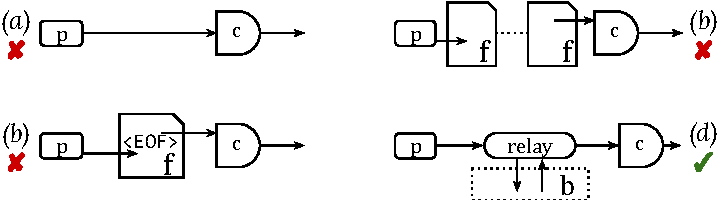
\includegraphics[width=0.49\textwidth]{\detokenize{./figs/dish_eager.pdf}}
\caption{
  \textbf{Eager primitive.}
  Describe three problems:
    (i) FIFOs alone cannot solve it as they’re blocking;
    (ii) intermediary files alone lose data, as the consumer reaches EOF before the producer; and
    (iii) writing to files + wait does not allow trask-based parallelism.
  Eager is an elegant solution that solves the problem while remaining within
  the model. Describe. \TODO{Combine this figure with the above code maybe.}
}
\vspace{-15pt}
\label{fig:eager}
\end{figure}


\heading{Split node implementation}


\noindent
\TODO{Problem: Pipeline width shrinks after pure commands. Solution:
  Split node that resplits its input to multiple files in sequence (to
  preserve the model semantics).}


%% Old and obsolete

%% \noindent
%% It is common in the dataflow graph for a node to have many incoming
%% edges or many outgoing edges (when all but the last outgoing edges
%% are bounded). However some nodes, might only read their input from one
%% source (e.g. stdin). In this case, the distributed implementation
%% needs to concatenate input files (or conversely split output
%% files).
%
%% \tr{Show an example graph! of cat | tr | sort. The command in the
%%   middle must only take input from one file (maybe just stdin).}
%
%% We address this issue using primitive shell constructs for file
%% manipulation. More concretely a merger can be implemented by means of a simple
%% \ttt{cat}. Given a set of input files \ttt{in1, in2, ...} and an
%% output file \ttt{out}, a merger can be implemented as:

%% \begin{lstlisting}[language=sh, numbers=none]
%%  cat $in1 $in2 ... > $out
%% \end{lstlisting}

%% \noindent
%% On the other hand, given an input file \ttt{in} that is a FIFO pipe,
%% and two output files \ttt{out1, out2} the first of which is bounded
%% to \ttt{|N} lines, a 2-splitter can be implemented as:

%% \begin{lstlisting}[language=sh, numbers=none]
%%   tee >(head -n $N > $temp1;
%%         dd of=/dev/null > /dev/null 2>&1 &
%%         cat $temp1 > $out1) |
%%        (tail -n +${N+1} > $out2;
%%         dd of=/dev/null > /dev/null 2>&1)
%% \end{lstlisting}
 %% head -n $N $in > $out1 ; cat $in > $out2

%% \noindent
%% Using the 2-splitter as a building block, a pipe can be split to
%% arbitrarily many different pipes.

\TODO{Talk about eagerness in split and how we needed to add eager
  nodes to n-1 outputs.}



\heading{Dangling FIFOs and Zombie Producers}

%% \TODO{(This problem is a nice followup for the one above) Problem:
%%   Dataflow graph termination. Illustration: Show the example of head
%%   deadlock and explain that this is inherent behaviour in the shell.
%%   (Solution: emptying pipelines or terminating processes) In order for
%%   things to terminate gracefully, dish wraps all commands in order to
%%   always consume all of their input by sending it down to
%%   /dev/null. Warning: This means that all commands in the pipeline
%%   must terminate gracefully if all of their output is consumed (if a
%%   process dies unexpectedly, noone will consume its input. We leave
%%   addressing that and other monitoring questions for future work). We
%%   evaluate the overhead of emptying all outputs in section X.}

% \nv{I think all of these titles should be the problem/challenge, not the solution}
% A process writing to a pipe needs to be notified when its consumer exits early before consuming all its output.
Under normal operation, a producer exits after it has produced and
sent all of its output to a pipe\todo{/its output channel}.
% \ttt{SIGPIPE} 
However, if its consumer exits early, the producer needs to be
notified so that it stops \todo{appending to the stream/trying to push
  data to its output channel}.
% ---so that it avoids unnecessary work and buffering challenges in the kernel.
In \unix, this is achieved by an out-of-band error mechanism:
  the operating system will deliver a \ttt{PIPE} signal to the producer, notifying it that the pipe's consumer has exited.
This is different from errors for other system calls return an error and unusual compared to non-\unix systems\footnote{
  For example, Windows indicate errors for \ttt{WriteFile} by its return code---similar to \ttt{DeleteFile} and other Win32 functions.
}
primarily because pipes and pipelines are at the heart of its philosophy.
% write errors are communicated differently 
Unfortunately though, if a pipe has not been opened for writing yet---which is possible for named pipes\kk{I think that it is also possible for anonymous, e.g. \ttt{cat f1 - | head -n 1}}---\unix cannot signal this condition.
Consider the following emitted code from \sys's earlier versions:\kk{Proposed alternative: ``Consider the following shell script:''}
\begin{lstlisting}[language=sh, numbers=none]
  mkfifo fifo1 fifo2
  cat file-chunk1.txt > fifo1 &
  cat file-chunk2.txt > fifo2 &
  cat fifo1 fifo2 | head -n 1 & wait
\end{lstlisting}
\noindent
In the code above, \ttt{head} exits early causing the last \ttt{cat} to exit before opening \ttt{fifo2}.
As a result, the second \ttt{cat} never receives a \ttt{PIPE} signal that its consumer exited---after all, \ttt{fifo2} never even had a consumer.
This, in turn, leaves the second \ttt{cat} unable to make process, both (i) blocked unable to write output, and (ii) unaware that its consumer has exited.
Coupled with \ttt{wait} at the end, the entire snippet reaches a deadlock.

To solve this problem, \sys emits cleanup logic that operates from the
end of the pipeline and towards its start.  The emitted code first
gathers the IDs of the output processes and passes them as parameters
to \ttt{wait}; this causes \ttt{wait} to block only on the output
producers of the dataflow graph.  Right after \ttt{wait}, \sys inserts
a routine that delivers \ttt{PIPE} signals to any remaining processes
upstream.  This epilogue is repeated for every \todo{merge/join} point
in the transformed pipeline \kk{I don't understand the final sentence}.
% Earlier: need to define split (fork?) and merge (join?) points; this should be "up to next merge point upstream"

\kk{We have to remember to say that for this to work, all nodes in the
  graph must always open their outputs! If not, then this technique
  doesn't work, and we have to monitor if any node dies to do
  something with it. At the moment we ensure that by doing that in our
  nodes, and by assuming that all nodes that we handle do that.}

% not receiving an out-of-band signal about that.
% never terminating, but 
% never terminate while the entire pipeline is waiting for 
% \ttt{\& echo \$!} and \ttt{kill -PIPE}

% The generated program could also (i) have signal handlers (traps) for propagating signals
% down the process tree; (ii) incorporate (a simple) cleanup logic for not leaving dangling processes and
% intermediary files; (iii) generate a correct exit code, depending on its
% execution. All of this can be easily generated by the compiler.

\heading{Pure Fold Function Implementations}

\kk{Maybe say something about some of the pure fold functions that we
  implemented. Interesting examples include sort and wc.}

%% The optimizer also applies custom transformations on several commands in \pur
%% to further improve their performance. Two notable examples are the
%% transformations on \ttt{sort} and \ttt{wc}. Occurences of \ttt{sort}
%% that have more than one input are tranformed to \ttt{sort} commands on
%% each input, followed by a \ttt{sort -m}, to produce the final sorted
%% result. The transformation on occurences of \ttt{wc} that have more
%% than input \ttt{i1, t2} is illustrated below as a shell script:
%% % \nv{do not understand i1, t2}

%% \begin{lstlisting}[language=sh, float=h, numbers=none, escapeinside={($}{$)}]
%%   paste -d '+' \
%%    <(wc i1 | tr -s ' ' '\n' | tail -n +2) \
%%    <(wc i2 | tr -s ' ' '\n' | tail -n +2) |
%%    bc | tr -s '\n' ' ' |
%%    sed 's/^/   /' | sed 's/$/\ /'
%% \end{lstlisting}

%% The above script takes the outputs produced by two \ttt{wc} commands
%% and aggregates them accordingly.



\section{Evaluation}
\label{eval}

\TODO{Remember to mention that deathstar has 128 threads but 64
  cores. So it is reasonable for the speedup to not go further in cpu
  heavy pipelines.}

\TODO{Should we mention that we empirically show that pash produces
  correct code?}

% FIXME
% \kk{We should make sure to measure the time that it takes for the
%   whole process to run (parsing, translating, optimizing, planning)
%   together with the scripts. This will probably be negligible, but we
%   still have to mention it. }
% 
% \kk{Also, we have to have one-two handcrafted examples that have more
%   than one pipeline, to show the execution time end to end, as this
%   cannot be shown with the one-pipeline examples since they only have
%   one graph, so no back and forth between shell and dish.}
% 
% \kk{Furthermore it would be great to have one distributed example that
%   runs in more than one node (if we have time)}
% 
% \kk{Also we have to make sure to measure with and without the final
%   cat of output file, so that we show that this is also negligible.}
% 
% \kk{We have to make sure that we repeat that the results are the same
%   in all tests that we run. Corectness, blah blah ...}
% 
% \kk{We should have at least some pipelines that have a bad pure
%   command in them.}


\begin{table*}[t]
\center
\footnotesize
% \setlength\tabcolsep{3pt}
\caption{
  \footnotesize{
    \textbf{Summary of shell one-liners}.
    The shell one-liners are small pipelines (\ie ones developed on-the-fly) drawn from various sources and applied to large datasets.
  }
}
%% \begin{tabular*}{\textwidth}{l @{\extracolsep{\fill}} llllll}
%% \toprule
%%   Script                 ~&~ Structure                    & Input (MB)& Time (Seq)    & Script Size (LoC)             & Highlights                                        \\
%% \midrule
%% % https://github.com/andromeda/sdsh/blob/master/scripts/grep.sh
%%   \tti{grep}         ~&~$3\times$\tsta                & 1000      &  78m 36.77s   &   30\qquad 134\qquad  1304    & complex NFA regex                                 \\
%% % https://github.com/andromeda/sdsh/blob/master/scripts/minimal5.sh
%%   \tti{sort}         ~&~~$\tsta, \tpur$               & 10000     &  23m 19.85s   &   33\qquad 129\qquad  1209    & \tti{sort}ing                                     \\
%% % https://github.com/andromeda/sdsh/blob/master/scripts/topn.sh
%%   \tti{wf}               ~&~~$3\times\tsta, 3\times\tpur$ & 1000      &   2m 11.18s   &   53\qquad 181\qquad  1621    & double \tti{sort}, \tti{uniq} reduction           \\
%% % https://github.com/andromeda/sdsh/blob/master/scripts/topn.sh
%%   \tti{top-n}            ~&~~$2\times\tsta, 4\times\tpur$ & 1000      &   6m 53.55s   &   53\qquad 181\qquad  1621    & double \tti{sort}, \tti{uniq} reduction           \\
%% % https://github.com/andromeda/sdsh/blob/master/scripts/ngrams.sh
%%   \tr{\tti{bi-gram}          ~&~~$2\times\tsta, 4\times\tpur$ & \todo{X}  &               &   X \qquad  X \qquad          & stream shifting and merging                       \\}
%% % https://github.com/andromeda/sdsh/blob/master/scripts/spell.sh
%%   \tti{spell}            ~&~~$4\times\tsta, 3\times\tpur$ & 1000      &   8m 13.42s   &  37 \qquad 257\qquad  2417    & comparisons (\tti{comm})                          \\
%% % https://github.com/andromeda/sdsh/blob/master/scripts/diff.sh
%%   \tr{\tti{diff}             ~&~~$4\times\tsta, 3\times\tpur$ & \todo{X}  &               &   X \qquad  X \qquad          & shuffling and non-distributable \tti{diff}ing     \\}
%%   \tti{shortest-scripts} ~&~~$5\times\tsta, 2\times\tpur$ & 8.6       &   2m 50.03s   &  61 \qquad 253\qquad  2413    & extensive file-system operation   \\
%% \bottomrule
%% \end{tabular*}
\begin{tabular*}{\textwidth}{l @{\extracolsep{\fill}} lllllll}
\toprule
Script ~&~ Structure & Input &Seq. Time & \#Nodes(16, 64) &Compile Time (16, 64) & Highlights \\
\midrule
\tti{grep} ~&~ $3\times\tsta$ & 1~GB & 79m35.197s & 49\qquad 193 & 0.056s\qquad 0.523s & complex NFA regex \\
\tti{sort} ~&~ $\tsta, \tpur$ & 10~GB & 21m46.807s & 77\qquad 317 & 0.090s\qquad 1.083s & \tti{sort}ing \\
\tti{top-n} ~&~ $2\times\tsta, 4\times\tpur$ & 10~GB & 78m45.872s & 96\qquad 384 & 0.145s\qquad 1.790s & double \tti{sort}, \tti{uniq} reduction \\
\tti{wf} ~&~ $3\times\tsta, 3\times\tpur$ & 10~GB & 22m30.048s & 96\qquad 384 & 0.147s\qquad 1.809s & double \tti{sort}, \tti{uniq} reduction \\
\tti{grep-light} ~&~ $3\times\tsta$ & 100~GB & 1m38.212s & 49\qquad 193 & 0.031s\qquad 0.163s & \todo{light computation} \\
\tti{spell} ~&~ $4\times\tsta, 3\times\tpur$ & 3~GB & 25m7.560s & 69\qquad 261 & 0.104s\qquad 1.038s & comparisons (\tti{comm}) \\
\tti{shortest-scripts} ~&~ $5\times\tsta, 2\times\tpur$ & 85~MB & 28m45.900s & 142\qquad 574 & 0.328s\qquad 4.657s & \todo{extensive file-system operation} \\
\tti{diff} ~&~ $2\times\tsta, 3\times\tpur$ & 10~GB & 25m49.097s & 125\qquad 509 & 0.186s\qquad 2.341s & non-parallelizable \tti{diff}ing \\
\tti{bi-grams} ~&~ $3\times\tsta, 3\times\tpur$ & 3~GB & 38m9.922s & 109\qquad 445 & 0.146s\qquad 1.716s & stream shifting and merging \\
\tti{optimized bi-grams} ~&~ $3\times\tsta, \tpur$ & 3~GB & 38m21.501s & 63\qquad 255 & 0.117s\qquad 1.482s & optimized version of bigrams \\
\tti{set-diff} ~&~ $5\times\tsta, 2\times\tpur$ & 10~GB & 51m32.313s & 155\qquad 635 & 0.321s\qquad 4.358s & two pipelines merging to a \tti{comm} \\
\tti{sort-sort} ~&~ $\tsta, 2\times\tpur$ & 10~GB & 31m26.147s & 78\qquad 318 & 0.092s\qquad 1.077s & parallelizable \tpur after \tpur \\
\bottomrule
\end{tabular*}

\label{tab:eval}
\end{table*}

\kk{Maximum scaleup for both diff and set-diff is around half because
  they already have two sorts running in parallel (as diff, and comm
  take two inputs).}

%% \TODO{Explain the plots with eager/no-eager as follows. Say that we
%%   initially decided to only make an eager version of cat (to allow for
%%   parallelism). However, we saw that results are still not good, so we
%%   resorted to making a proper generic eager node that can be put
%%   anywhere in the graph and that eagerly consumes its input. The above
%%   results show the improvement with it. Rerun them with eager only
%%   before cat in the no eager cases so that the minimal-grep example is
%%   the same with and without our eager node.}

\TODO{(Maybe) we need to mention that eager has disk usage overhead
  that is linear to the size of the pipeline and the size of the
  input.}


At a high level, we are interested in understanding whether \sys can indeed scale pipelines out automatically and correctly.
To achieve this, we use six micro-benchmarks and one macro-benchmark, collected primarily from prior literature.

Micro-bench\-marks~\sx{ours} are one-off, simple one-liners that take a few seconds to write;
  such pipelines are usually composed interactively to solve a task at hand, test a hypothesis, or ``smoke out bugs''~\cite{bentley1986literate}---but, with \sys, applied to very large data sets.
These pipelines are taken from real use cases~\cite{bentley1985spelling, bentley1986literate, taylor2004wicked} and, precisely due to their small size, highlight stress on a handful of stages.

The complex macro-benchmark (\S\ref{macro1}) is designed to handle realistic workloads by today's standards.
It is about an order of magnitude larger than the micro-benchmarks, but its perceived lack of complexity is deceiving:
  as shown, if written in a conventional language it would correspond to a program on the order of hundreds of lines of code.

Several results are worth highlighting.
First, programs see a significant speedup, often more $10\times$ over sequential execution  while returning identical results (on very large datasets).
\sys's transformation and planning phase take around 50--300ms, negligible ($<$2\%) for short-running pipelines and virtually non-existent for long-running ones.
As \sys rewrites to highly-optimized shell primitives rather than using a managed language runtime, it always has a COST~\cite{mcsherryscalability} of 2.
Finally, \sys preserves the productivity of the shell:
  the equivalent program for a small part of the macro-benchmark pipeline requires over a 150 lines of code in combined Java and Bash to run distributed on top of Hadoop.
  %% in another, the program expressed by the pipeline was the subject of a semester project in a graduate course on distributed systems~\cite{blinded} where student implementations ranged between 1--3\textbf{K} lines of code.

Experiments were run on a %\todo{network of five workstations} connected by 1Gbps links: 
  machine with 512GB of memory and 128 virtual (64 physical) $\times$ 2.1GHz Intel Xeon E5-2683 cores.
%\todo{four smaller machines (\wkq), each with 4GB of memory and two 3.33GHz Intel Core Duo E8600 processors}.
For our software setup, we use Debian 4.9.144-3.1, GNU Core-utils 8.30-3, GNU Bash 5.0.3(1)-, Python 3.7.3, and OCaml 4.05.0.
Generally, no special configuration was made in hardware or software.
All pipelines are set to (initially) read from and (finally) write to the file-system (except as otherwise stated).
Whenever \ttt{curl} is part of a pipeline, it fetches data from a different physical host on the same network connected by 1Gbps links.
A more detailed description of the setup and experiments, including reproducible scripts, is included in the accompanying (anonymized) online repository.

\subsection{Common \unix One-liners}
\label{ours}

The goal of this subsection is to evaluate \sys on popular, common, or classic \unix pipeline patterns.

\begin{figure*}[t]
    \centering
    %% \subcaptionbox{\label{eval:minimal_grep}}{
    %%     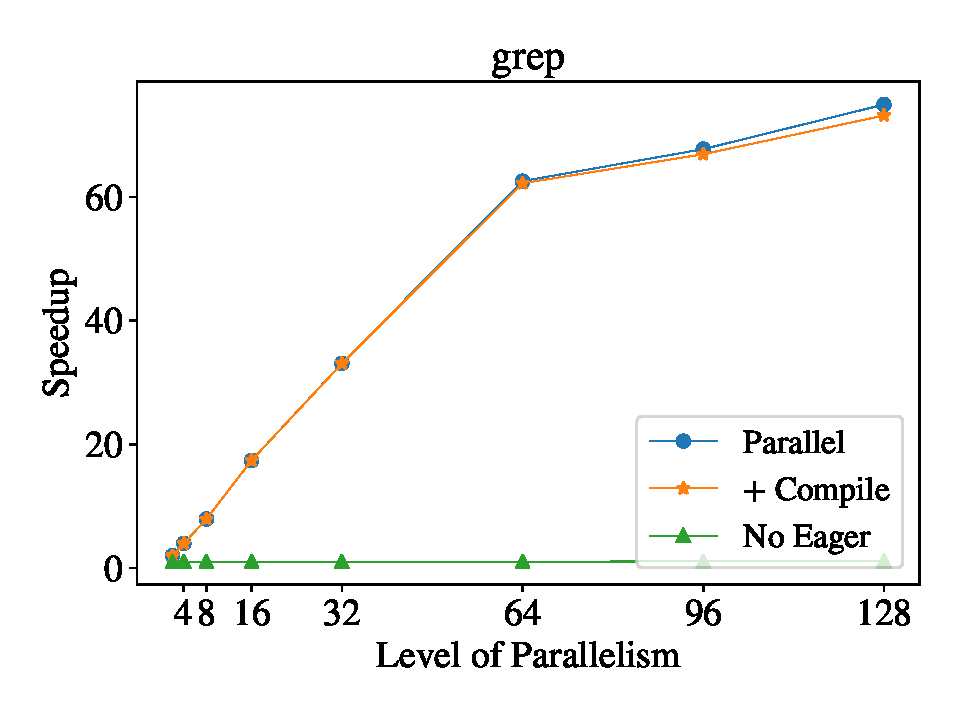
\includegraphics[width=0.32\textwidth]{\detokenize{./figs/minimal_grep_throughput_scaleup.pdf}}
    %% }
    %% \subcaptionbox{\label{eval:grep}}{
    %%     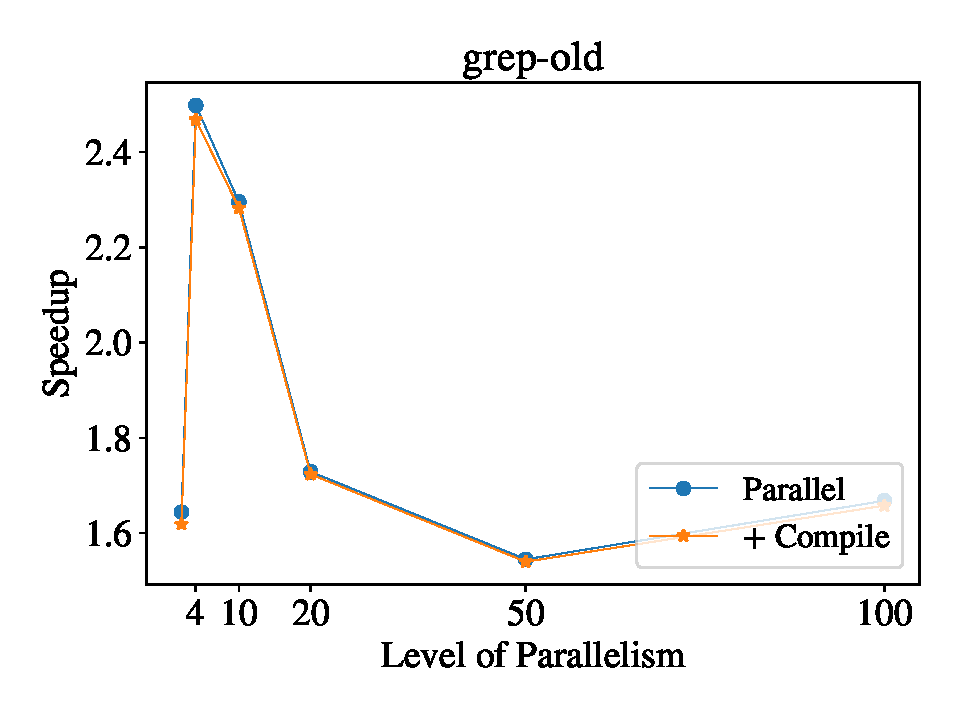
\includegraphics[width=0.32\textwidth]{\detokenize{./figs/grep_throughput_scaleup.pdf}}
    %% }
    %% \subcaptionbox{\label{eval:minimal_sort}}{
    %%     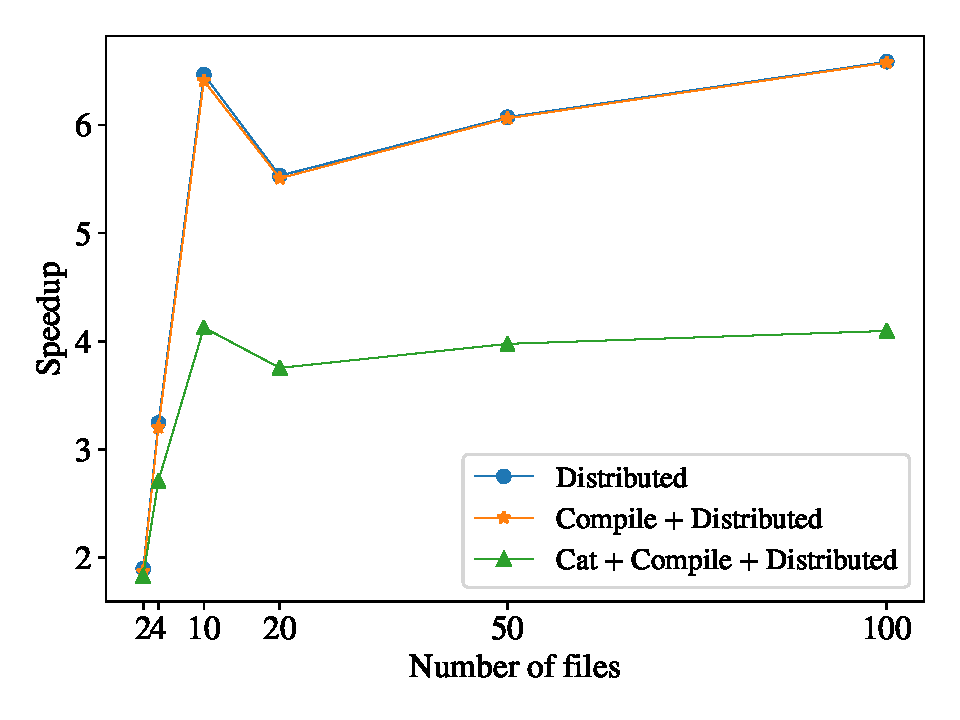
\includegraphics[width=0.32\textwidth]{\detokenize{./figs/minimal_sort_throughput_scaleup.pdf}}
    %% }
    %% \subcaptionbox{\label{eval:topn}}{
    %%     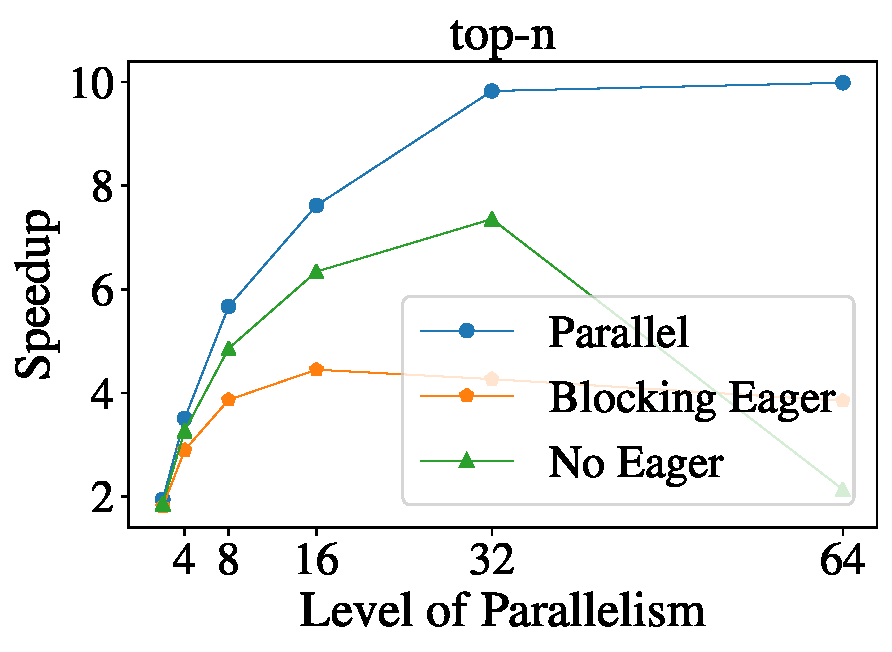
\includegraphics[width=0.32\textwidth]{\detokenize{./figs/topn_throughput_scaleup.pdf}}
    %% }
    %% \subcaptionbox{\label{eval:wf}}{
    %%     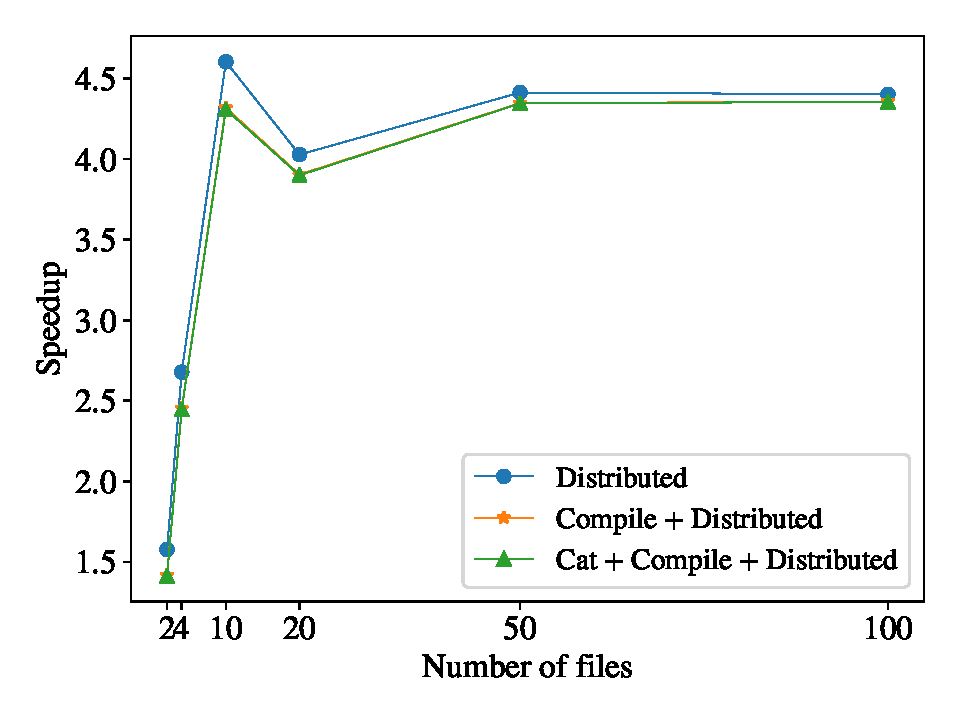
\includegraphics[width=0.32\textwidth]{\detokenize{./figs/wf_throughput_scaleup.pdf}}
    %% }
    %% \subcaptionbox{\label{eval:spell}}{
    %%     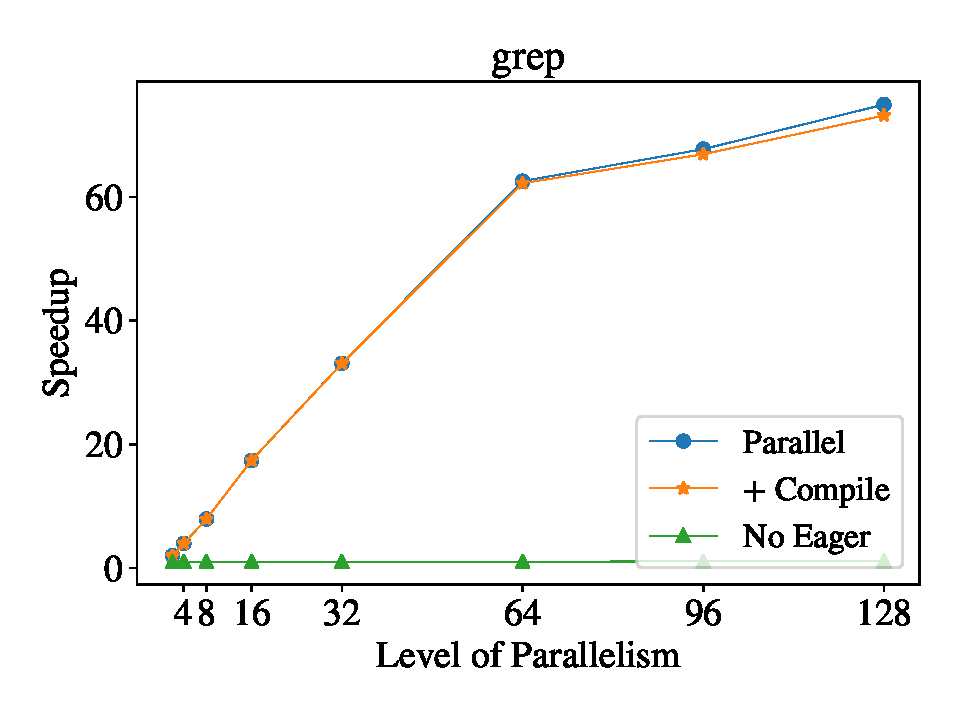
\includegraphics[width=0.32\textwidth]{\detokenize{./figs/minimal_grep_throughput_scaleup.pdf}}
    %% }
    %% \caption{a}
    \begin{subfigure}[b]{0.24\textwidth}
        \centering
        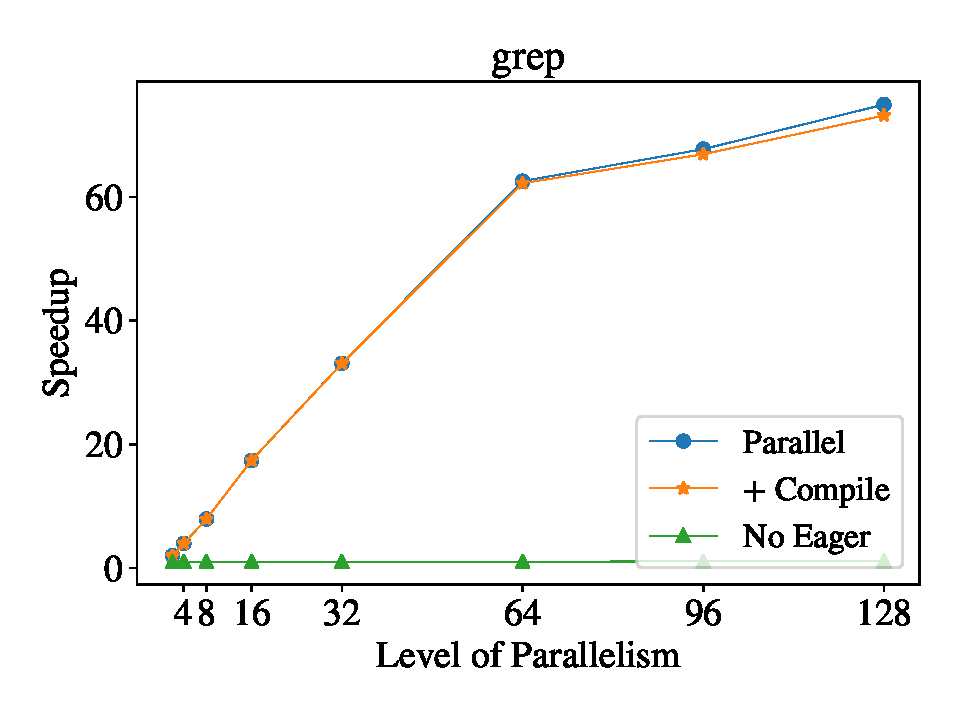
\includegraphics[width=\textwidth]{\detokenize{./figs/minimal_grep_throughput_scaleup.pdf}}
        %% \caption{TODO}
        %% \label{eval:minimal_grep}
    \end{subfigure}%
    ~
    \begin{subfigure}[b]{0.24\textwidth}
        \centering
        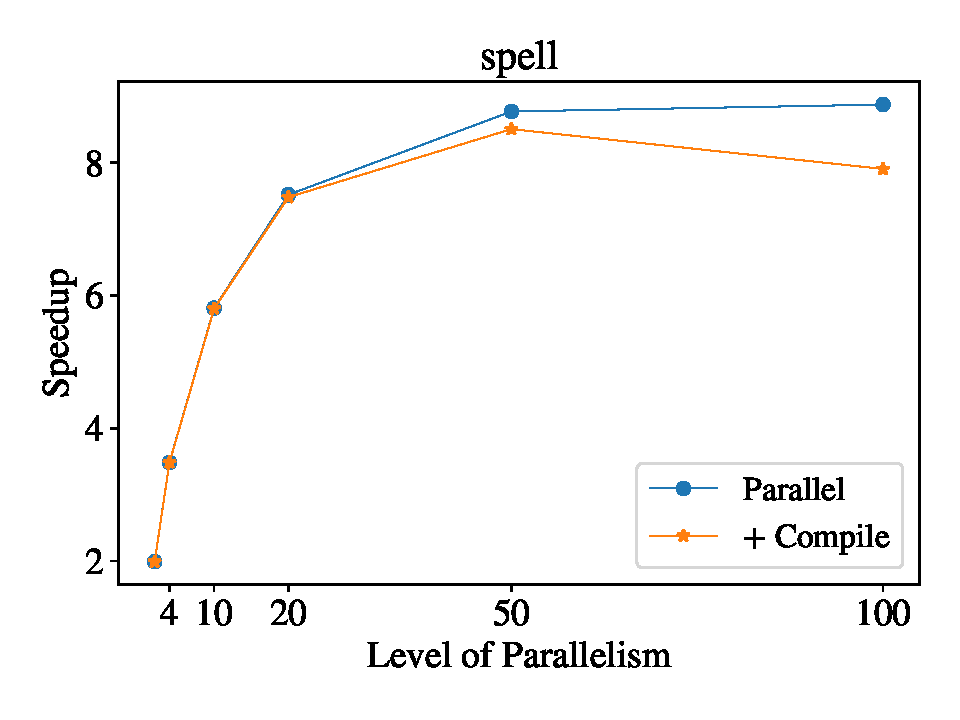
\includegraphics[width=\textwidth]{\detokenize{./figs/spell_throughput_scaleup.pdf}}
        %% \caption{TODO}
        %% \label{eval:grep}
    \end{subfigure}%
    ~
    \begin{subfigure}[b]{0.24\textwidth}
        \centering
        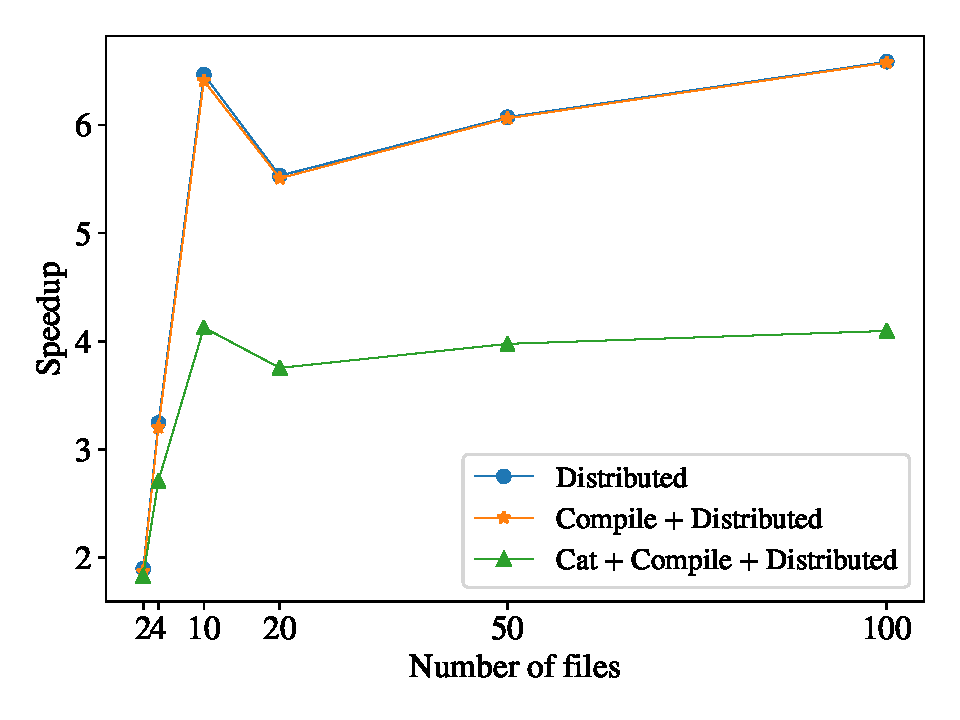
\includegraphics[width=\textwidth]{\detokenize{./figs/minimal_sort_throughput_scaleup.pdf}}
        %% \caption{TODO}
        %% \label{eval:minimal_sort}
    \end{subfigure}%
    ~
    \begin{subfigure}[b]{0.24\textwidth}
      \centering
      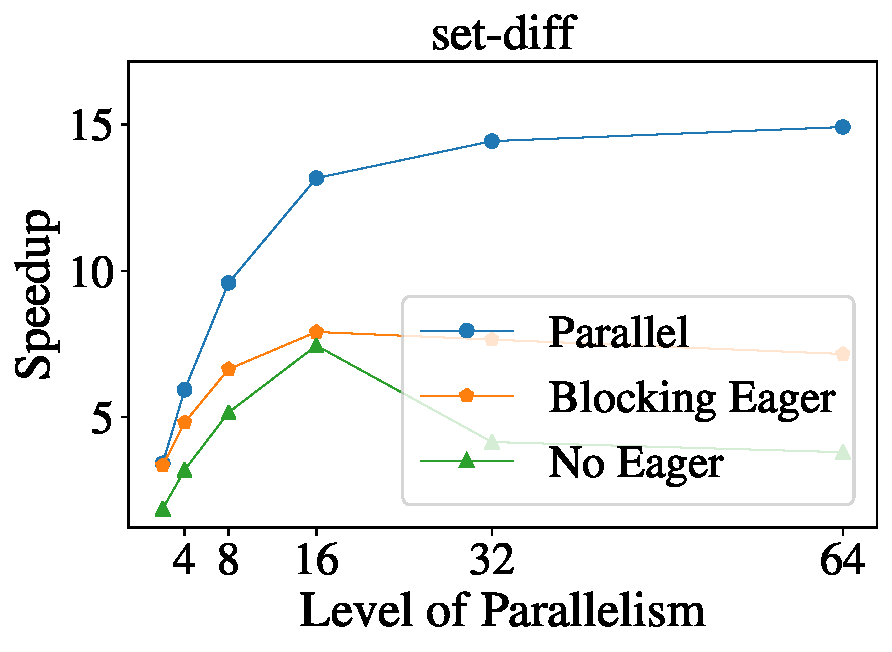
\includegraphics[width=\textwidth]{\detokenize{./figs/set-diff_throughput_scaleup.pdf}}
        %% \caption{TODO}
        %% \label{eval:minimal_sort}
    \end{subfigure}%

    \begin{subfigure}[b]{0.24\textwidth}
        \centering
        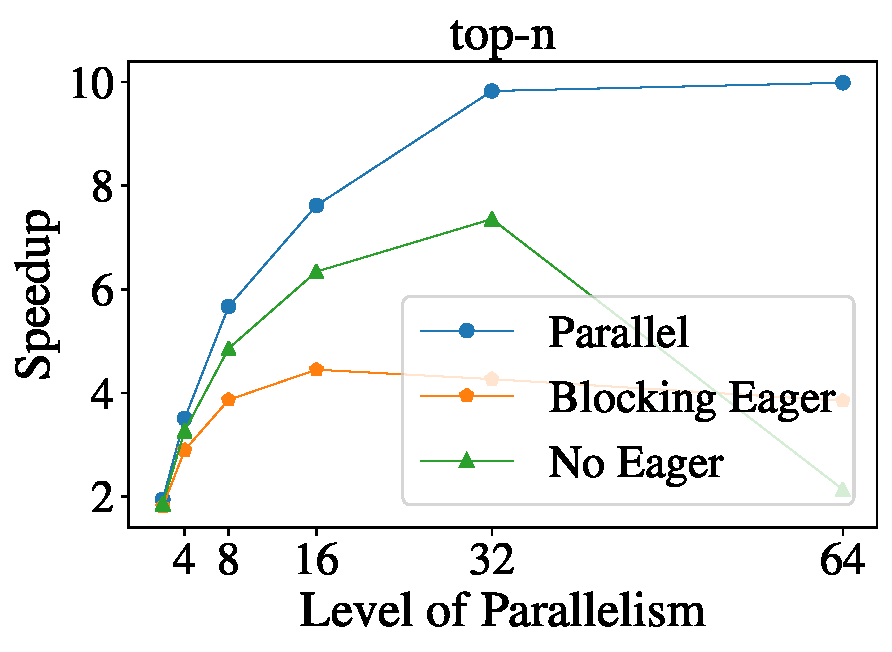
\includegraphics[width=\textwidth]{\detokenize{./figs/topn_throughput_scaleup.pdf}}
        %% \caption{TODO}
        %% \label{eval:topn}
    \end{subfigure}%
    ~
    \begin{subfigure}[b]{0.24\textwidth}
        \centering
        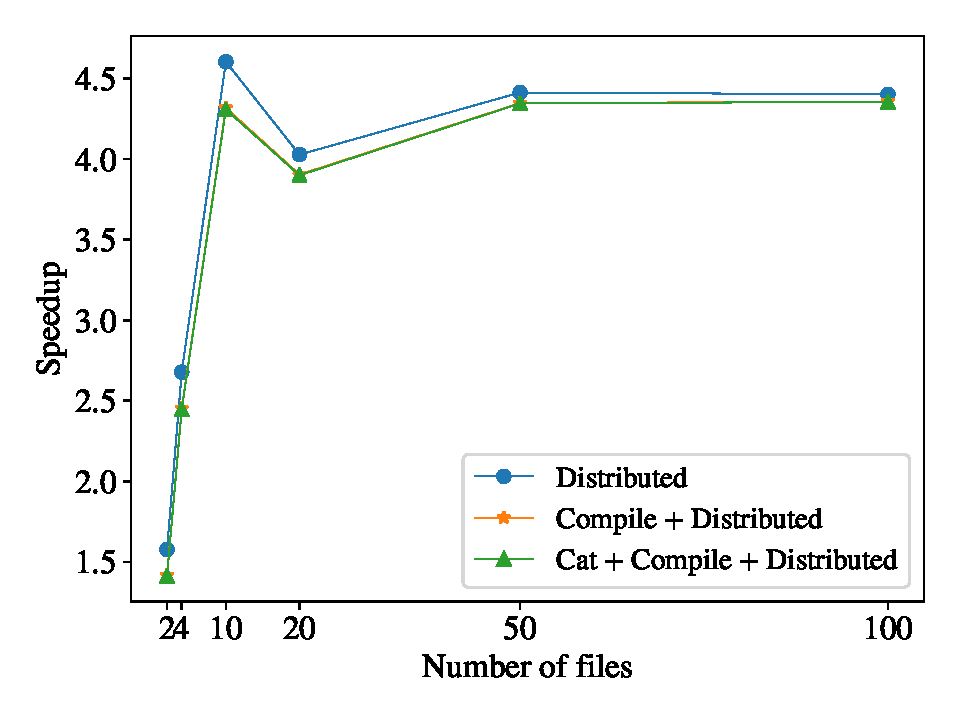
\includegraphics[width=\textwidth]{\detokenize{./figs/wf_throughput_scaleup.pdf}}
        %% \caption{TODO}
        %% \label{eval:wf}
    \end{subfigure}%
    ~
    \begin{subfigure}[b]{0.24\textwidth}
        \centering
        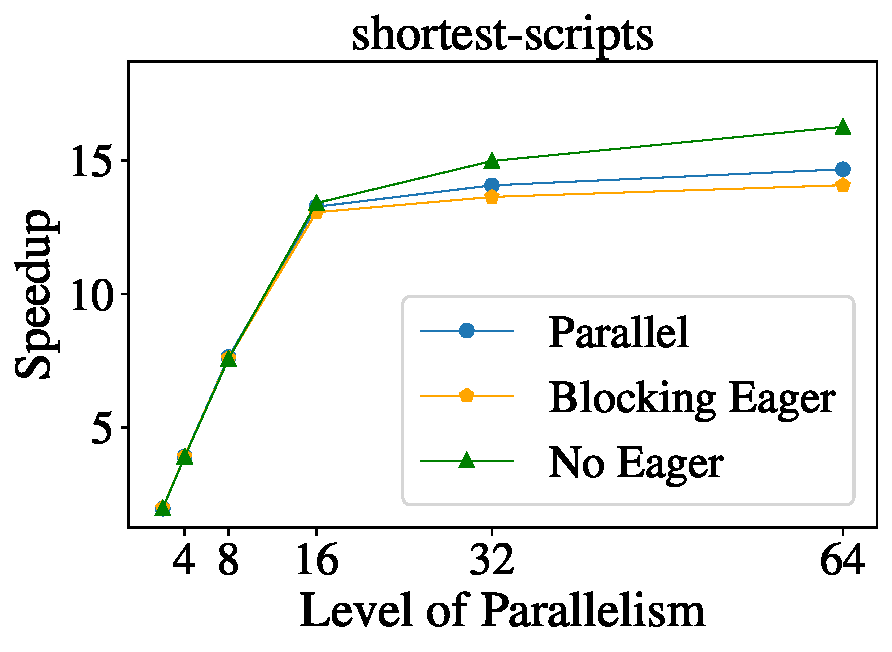
\includegraphics[width=\textwidth]{\detokenize{./figs/shortest_scripts_throughput_scaleup.pdf}}
        %% \caption{TODO}
        %% \label{eval:spell}
    \end{subfigure}%
    ~
    \begin{subfigure}[b]{0.24\textwidth}
      \centering
      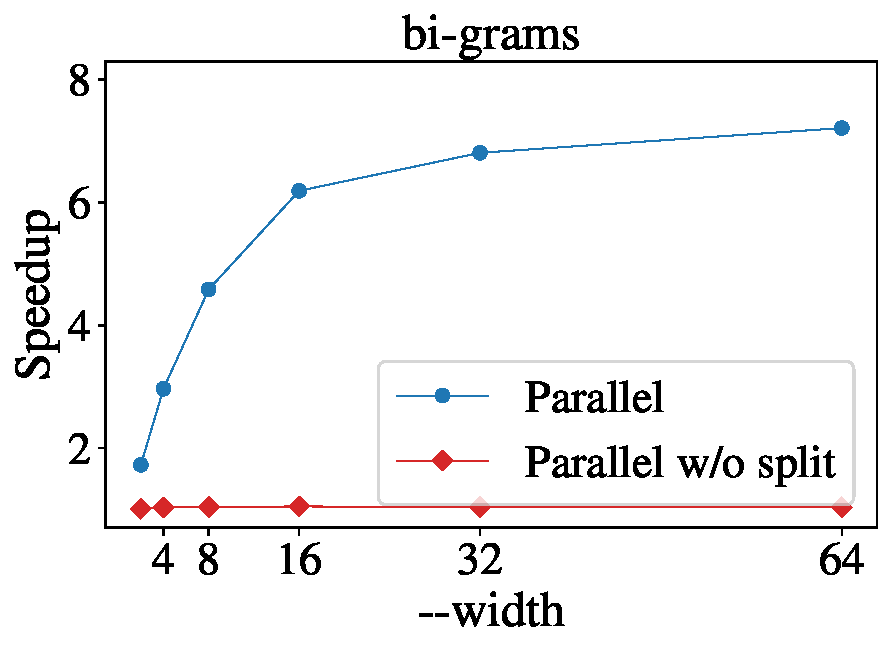
\includegraphics[width=\textwidth]{\detokenize{./figs/bigrams_throughput_scaleup.pdf}}
        %% \caption{TODO}
        %% \label{eval:minimal_sort}
    \end{subfigure}%
    \caption{
      \textbf{Speedup achieved by \sys as a function of the level of parallelism (1--100).} 
      Four different configurations per benchmark:
      (i) \todo{Par + Split}, showing the performance of \sys with both eager and split optimizations enabled,
      (ii) \todo{Par + B. Split}, showing the performance of \sys with eager and the \todo{batch-size annotated} split optimizations enabled,
      (ii) \todo{Parallel}, showing the performance of \sys with eager enabled and split disabled,
      (iii) \todo{No Eager}, showing the performance of \sys with split and eager disabled,
      (iv) \todo{Blocking Eager}, showing the performance of \sys with split disabled and the naive blocking eager enabled,
      \nv{Maybe it makes sense to show log x-axis?}
      \kk{How can we also fit two more plots (sort-sort and diff) here? Maybe we can fit one by getting rid of sort (since it also shown in the sort--parallel one). Otherwise we could separate the ``split'' plots from the ones that don't have split.}
    }
    \vspace{-15pt}
    \label{fig:microbenchmarks}
\end{figure*}

\heading{Programs}

\kk{How can we include a result for grep-light?  This is the IO
  intensive CPU-light grep. \sys has no speedup but also no slowdown
  (even if it IO heavy). Should we just mention that in text in
  passing?}

\kk{Remember to mention that for spell and bigrams we dont show other
  parallel because they are all close to 1 (no speedup).}

Tab.~\ref{tab:eval} summarizes the collection of micro-benchmarks used to evaluate \sys.
Benchmark names (col. 1) correspond to the names on the plots (Fig.~\ref{fig:microbenchmarks}), and structure (col. 2) summarizes the different classes of commands used in the script.
% The centralized pipelines read files of various sizes from disk and write to disk.
Input sizes and times (col. 3, 4) summarize the characteristics of the largest sequential executions. % (200 files in Fig.~\ref{fig:microbenchmarks}).
Script sizes (col. 5) report on \sys's rewritten output for three different distribution sizes---$1\times$, 10$\times$, and $100\times$.
Size grows due to the resulting complexity of coordinating among parallel executions---multiple FIFOs per pipeline stage, merging and splitting, encoding of divide-and-conquer synchronization \etc
The first number alone is interesting, as it captures \sys's output for the sequential script.
As there is no parallelism involved, it highlights the initial (bare minimum) cost corresponding to using \sys.
% this is the size of 
This change in size does not necessarily translate to observed runtime, as most of the size increase comes from the setup and teardown of FIFOs responsible for interprocess (IPC) communication.
FIFOs are simply pipes made explicit;
  the performance characteristics, including in-kernel buffering and synchronization mechanisms, are identical between the two.

In more detail, \ttt{grep} is a short script centered around an expensive \tsta command;
% a DFA-based regular expression matching phase;
  while the \unix \ttt{grep} command defaults to a Thompson NFA, this particular expression makes use of DFA-based backtracking patterns resulting in high runtime overhead.
The \ttt{sort} pipeline is equally short, but its central operation is a command in \pur.
The next two benchmarks, \ttt{wf} and \ttt{top-n}, are based on McIlroy's now classic word-counting program~\cite{bentley1986literate};
  they use sorting, rather than tabulation, to identify high-frequency terms in a corpus.
% \tr{The \ttt{bi-gram} pipeline calculates n-grams of base two;
%   it makes clever use of \ttt{tail} to shift a stream by one word and \ttt{paste} to fuse (zip) two streams together.}
The next pipeline is based on the original \ttt{spell} program developed by Johnson~\cite{bentley1985spelling}---another \unix classic:
  after some preprocessing, it makes clever use of \ttt{comm} to report words not in the dictionary.
Finally, \ttt{shortest-scripts} is a pipeline~\cite[pg. 7]{taylor2004wicked}that identifies the 15 shortest shell scripts in the user's \ttt{PATH};
   interestingly, it uses the \ttt{file} utility and a higher-order \ttt{wc} via \ttt{xargs}.

\heading{Performance}
% TODO \nv{Need to change terminology in plots---files should be (attempted) parallelism, name benchmark, cat should be merge.}
Fig.~\ref{fig:microbenchmarks} presents the speedup gained by \sys as a function of the level of parallelism (1--200$\times$).
% we experiment with a $200\times$ level of parallelism to see potential overheads
Each one of these plots reports on three different configurations:
  (i) distributed, which captures only the runtime of the distributed computation,
  (ii) +compile, which adds the \sys' analysis and generation overhead, and
  (iii) +merge, which adds a final merger  gathering the results at the end of the pipeline.
Parallelism of 200$\times$ was explicitly chosen to show the \sys-internal overheads on suboptimal configurations;
  \sys itself would never attempt a factor that is above the number of available compute nodes.
The results show significant speedups, ranging between 4--70$\times$, depending on the parallelizability characteristics of individual pipelines.

\heading{Discussion}
\kk{Below follows an important point about why scalability is more
  than great in the beginning and then gets worse.}
An interesting point is that \sys seems to achieve almost linear
speedup with small parallelism configurations. The reason why this
happens is not so straightforward though. \sys manages that because it
exploits task-based parallelism by having different processes to do
the \todo{map} and the \todo{reduce} phase. Due to task-based
parallelism in the generated dataflow graphs, \sys essentially ``uses
more parallelism'' than the given configuration. This can be seen in
all pipelines that are not completely stateless. For example, in the
\ttt{minimal\_sort} one-liner, \sys configured to have 8 parallelism
spawns 37 nodes (8 \ttt{tr} nodes, 8 \ttt{sort} nodes, 7 \ttt{sort -m}
nodes, and 14 \ttt{eager} nodes. This indicates that \sys achieves
optimal performance (without unnecessary process spawns and context
switches) in pipelines that contain pure commands by configuring it
with a smaller parallelism than the capabilities of the underlying
system -- in our case 16-32 for a 64 physical core system. This is
also the case if the input pipeline is very long and so there is
already task-based parallelism even in the sequential execution
(several of the Unix50 pipelines fall in this category).

\kk{Hypothesis on a scalability upper bound. Dish gives a great
  speedup if one step of the pipeline is what takes the most time. If
  the pipeline is long with many computation heavy tasks, task based
  parallelism gets you part of the way there, so we can't expect Dish
  to give performance benefits equal to the amount of parallelism that
  we give it.}

\TODO{Briefly discuss the performance drop as we increase parallelism
  in some one-liners (sort-sort, bi-grams).The reason has to do with
  context switching. More precisely, sort-sort 32 has 314 nodes (and
  54m sys time) and sort-sort 64 has 634 nodes (and 90m! sys time). On
  the other hand opt-bigrams 64 has 255 nodes and the sys time stays
  the same so I think that it might have to do with the fact that
  constant costs rise a lot (since opt-bigrams 32 takes just 1
  minute).}

\kk{It is visible that the automatic split is slightly worse than the
  manual one in most cases (because it doesn't utilize task-based
  parallelism).}

We attribute the small drop above $96\times$ in \ttt{spell} \ttt{sort} \ttt{wf}
and \ttt{bi-grams} to a combination of hyperthreading (128 virtual vs. 64
physical CPUs) \todo{the fixed width on} \ttt{sort}.
% I say "we attribute" because it's a way to say something without being certain
% FIXME: We need to take linear benchmarks on deathstar and livestar to see
% where it starts dropping
% not explain scope the results appropriately
% rinard

\heading{Take-aways}

\subsection{Unix50 from Bell Labs}
\label{unix50}

The goal of this subsection is to evaluate \sys on an existing set of \unix pipelines found in the wild.

\heading{Programs} In a recent event celebrating \unix's 50-year
legacy, Bell Labs created a set of \todo{36} challenges~\cite{unix50}
solvable by means of composing \unix pipelines.  By scanning GitHub,
we were able to find a set of shell programs that solve
\todo{all-but-three} problems~\cite{}.  We consider this a good set of
benchmarks because (i) the problems were designed to to highlight the
\unix philosophy~\cite{} (rather than having a single command that
solves the problem) and make extensive use of \unix built-ins with a
plethora of flags, and (ii) the solutions were written by non-experts
(contrary to the \S\ref{ours}) and were executed by \sys
unmodified---stressing patterns that we, \sys's authors, did not
necessarily anticipate \kk{I would change that to ``stressing a
  variety of patterns'' since it doesn't really matter if we
  anticipated them (especially since we can address any issues and
  then re-run them).} .  In cases where an obvious fix improves the
pipeline's performance, we report on both \sys's original speedup and
the one achieved by applying the fix.
% TODO: talk about correct wrt developer intentions vs. correct wrt problem definition

% The ability to compose larger programs in versatile ways from smaller utility programs was a hallmark of the \unix design, and the game's levels are designed to stress that.
% These challenges were specifically designed to highlight the \unix's philosophy, its 
% ability to compose larger programs in versatile ways from smaller utility programs summarized by McIllroy's Unix philosophy memo.

%% \TODO{An important point that needs to be made clear is that these are
%%   taken from the wild unmodified. And that Pash never leads to
%%   slowdown (except for the trivial head cases, where the slowdown is
%%   neligible).}

\heading{Results} \sys's parallelism set to 16. The input given to the
pipelines was the test input from unix50 multiplied to reach
10GBs. The speedup of each pipeline separately is shown in
\Cref{fig:unix50-individual}. The average\todo{/median} speedup is
$5.49$/\todo{$6.07\times$}, the \todo{geometric mean is $1.08\times$},
and the \todo{weighted average (with the absolute times as weights) is
  $5.75\times$}.

%% Mean: 5.499164686559543
%% Median: 6.075774436154179
%% Geometric Mean: 1.0798740409683736
%% Weighted Average: 5.752406752503295

\begin{figure}[t]
  \centering
  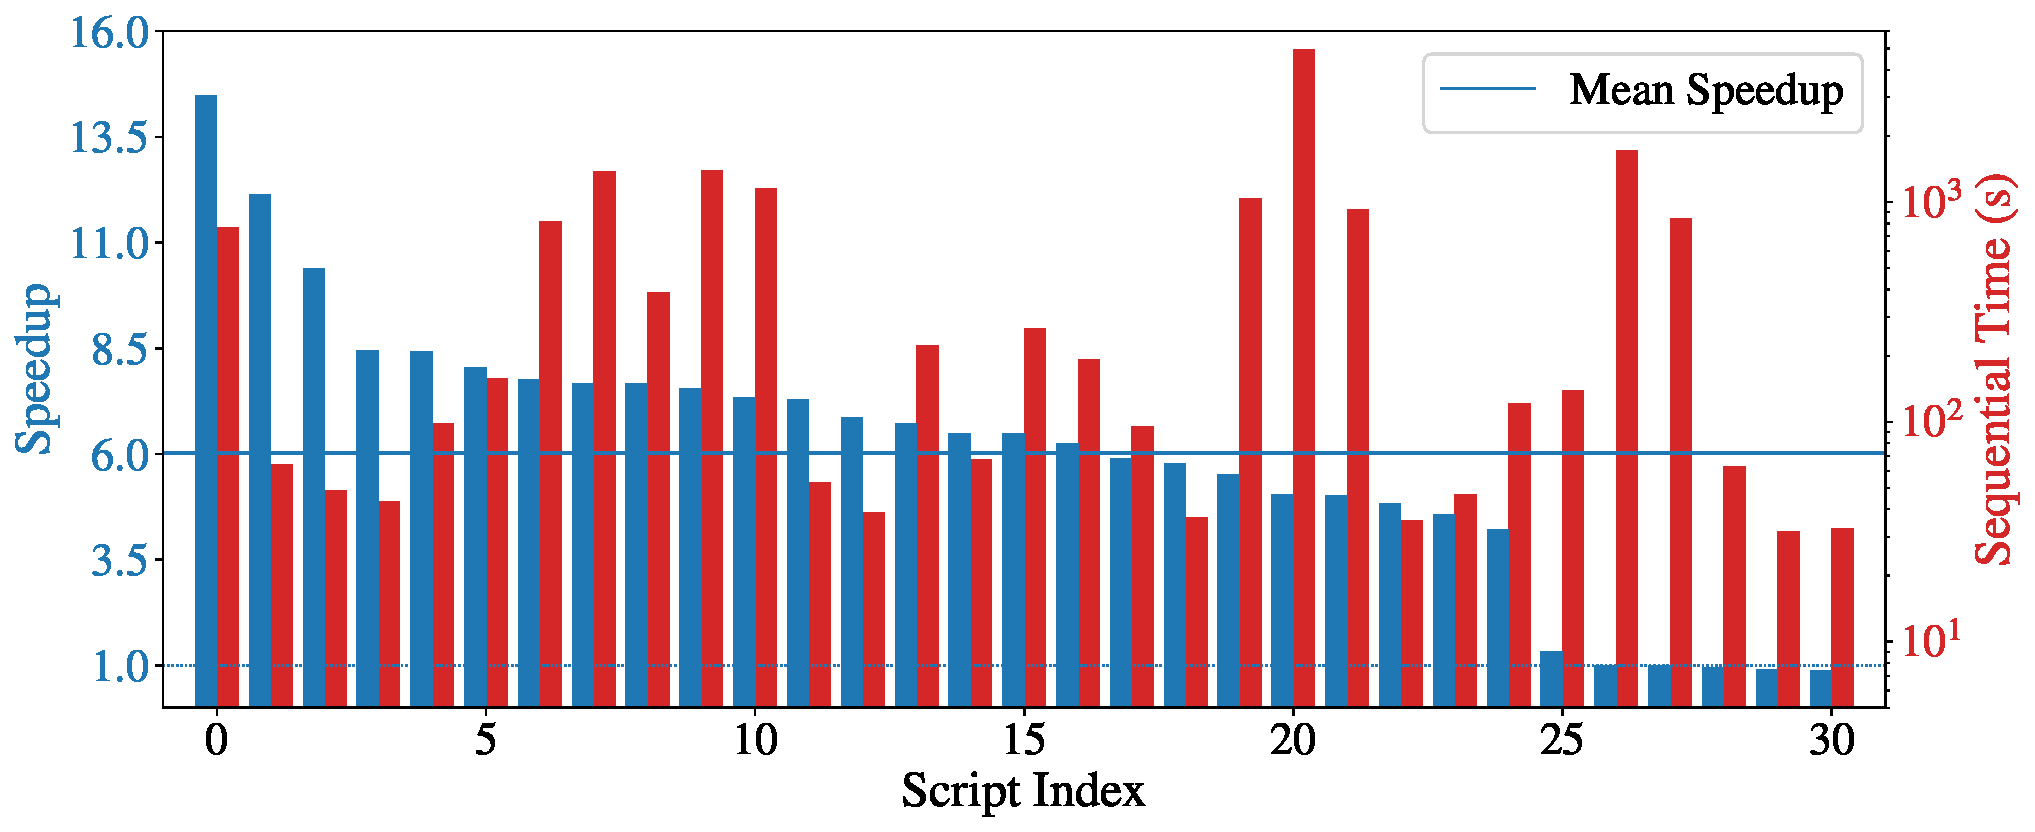
\includegraphics[width=\columnwidth]{\detokenize{./figs/unix50_individual_speedups_16.pdf}}
  \caption{
	  \textbf{Speedup (left axis) and over sequential execution (right axis) for all Unix50 pipelines.}
		Parallelism is 16$\times$ on 10GB of input data~\cf{unix50}.
  }
  \vspace{-15pt}
  \label{fig:unix50-individual}
\end{figure}


\heading{Discussion}

%% Breakdown of not ideal speedups in 8, 16 parallelism

%% Head: 2, 19, 31
%% Sort-bottleneck: 1, 3, 15, 16, 20, 33
%% Non-parallelizable completely: 13 (awk-solved), 18 (awk), 24, 25, 26, 29, 30
%% Cheap (non cpu intensive -- constant costs grow): 0, 4, 5, 6, 7, 8, 12, 14
%% Long (task-based parallelism in sequential and context switches): 7, 8, 9, 10, 11, 12, 14, 21, 27, 28

%% \kk{Out of all benchmarks, we have talked about the head and the
%%   non-parallelizable ones in the paper. Maybe we also want to talk
%%   about the long and the cheap ones. Also we might want to talk and
%%   find out more about the sort bottleneck.}


%% (OLD) Bad result descriptions:
%%  2. Contains just a head -n 2, and then a cut.
%%  5. Very fast (small input). Sequential time is 0m0.103s (If we increase the input we will show speedup)
%%  18. TODO: Implement
%%  20. Four corners (not parallelizable). So performance is reasonable
%%      (atm it doesn't return the correct result for multiplied input though)
%%  21. Last capital character of each line. Their solution is not general (and it is not parallelizable).
%%      Also, the input is very small. Changing it to a more general one and
%%      increasing input size leads to speedup. TODO: Run with large input
%%  22. Exactly the same problem as the above.
%%  24. (Not sure: It seems that the computation is trivial)
%%  32. TODO: Implement

\sys achieves speedup in all pipelines except for 2, 19, and 31. These
pipelines include a \ttt{head} and only process one line of the
input. This can be seen by their sequential execution time which is in
the order of 10 milliseconds. The slowdown is due to constant costs of
setting up the pipes and spawning processes. In all three of these
cases the execution time with \sys is in the order of 1 second. For
pipelines 13, 24, 25, 26, 29, and 30, \sys performs the same as the
sequential implementation. This is because these pipelines contain
commands that can not be parallelized in general, such as \ttt{awk},
\ttt{sed} with option \ttt{d}, and \ttt{tr} with option \ttt{-d}. An
illustrative example is pipeline 13, which is shown here:

\begin{lstlisting}[language=sh, float=h, numbers=none]
  cat $IN | awk "{print \$2, \$0}" |
      sort -nr | cut -d ' ' -f 2
\end{lstlisting}

\kk{Rephrase that to sound more meaningful and surprising.}  Notice
that \ttt{awk} is just used to permute two of the columns of the input
to enable sorting. One could write this pipeline in a different way,
by directly sorting on the second column:

\begin{lstlisting}[language=sh, float=h, numbers=none]
  cat $IN6 | sort -nr -k 2 | cut -d ' ' -f 1
\end{lstlisting}

By executing this version of the pipeline with \sys, we achieve
\todo{X} speedup. This indicates that just a little awaresess of
command parallelizability can go a long way, and that the effort that
a \sys user needs to spend is often negligible to achieve
benefits.

Finally, for the rest of the pipelines \sys speedup is \todo{capped}
because of a combination of the following reasons: (i) they contain
pure commands that are parallelizable but don't scale linearly, such
as \ttt{sort} (e.g. pipelines 0, 1, 3, 15, 16, 18, 20, 27, 28, 33),
(ii) they are deep pipelines that already exploit task-based
parallelism (e.g. pipelines 7, 8, 9, 10, 11, 12, 14, 27, 28), and
(iii) they are not cpu-intensive, leading to \todo{larger IO and
  constant costs} (e.g. pipelines 4, 5, 6, 7, 8, 12, 14, 22, 23).

%% Sort-bottleneck: 1, 3, 15, 16, 20, 33
%% Non-parallelizable completely: 13 (awk-solved), 18 (awk), 24, 25, 26, 29, 30
%% Cheap (non cpu intensive -- constant costs grow): 0, 4, 5, 6, 7, 8, 12, 14, 22, 23
%% Long (task-based parallelism in sequential and context switches): 7, 8, 9, 10, 11, 12, 14, 21, 27, 28

%% Finally, an important point that is reinforced from this
%% experiment is that \sys doesn't lead to slowdown, even in cases where
%% parallelism is not possible.



\heading{Take-aways} \sys leads to significant performance
improvements in completely unmodified \unix pipelines found out in the
wild. Small tweaks can yield further improvements, showing that
\sys-awareness and scripting expertise can improve
results. Furthermore, it doesn't cause slowdown in any non-trivial
computation, even in cases where parallelism is not possible.

\subsection{Use Case: NOAA Weather Analysis}
\label{macro1}

To understand \sys better under a realistic workload, we turn our attention to the Fig.~\ref{fig:example}'s script~\sx{bg}.

\heading{Program}
The full version of this program is inspired by the introductory chapter of Hadoop's Definitive Guide~\cite[Chapter 2]{hadoop:15}, where it is used as an example of a realistic mid-scale analytics pipeline.

The original task, as presented in the book, is comprised of three sub-tasks:
  download weather data from NCDC (shell), convert them to a format that is Hadoop-friendly (shell), and process them to identify the maximum temperature (Hadoop).
Only the last of these tasks is the real focus of the book, demonstrating the benefits of using distributed framework such as Hadoop.
For \sys, we consider the full pipeline that implements all three sub-tasks---from fetching data to outputting the maximum temperature.

The full program used for our evaluation is slightly different than the one presented in Fig.~\ref{fig:example}, consisting of 14 stages and totalling 240 characters.
We full program expresses the \ttt{for} loop as its first pipeline stage and uses \ttt{xargs} to 
The program presented in Fig.~\ref{fig:example} is simplified only for clarity of exposition.

\heading{Results}
% The first interesting result 
\TODO{Some results}
The Hadoop program, expressed in Java and only capturing the \emph{four} last stages, amounts to 137 lines of Java code---not accounting for commands moving data in and out of HDFS.

As this is benchmark is taken directly from the Hadoop book, it is worth reporting on its execution time.
While the setup is not typical of Hadoop, the comparison between the two systems is not unreasonable:  % we took several steps to make the comparison fair:
  (i) both Hadoop and Spark favor message-passing rather than shared memory,
	(ii) Hadoop has no fault-tolerance for master and worker nodes (\ie both systems do not replicate data),
	(iii) the task at hand is a good fit for  Hadoop,
	(iv) the Hadoop program is written as a single program tailored for this task---with ample opportunity for optimization from the compiler and runtime system---rather than a series of loosely coupled programs each written to handle many other cases.
\todo{The original pipeline executes in XXs---long enough to amortize Hadoop's 0.5--0.9s startup costs.}
With two Hadoop 3.2.1 (Openjdk 11.0.5) data-nodes, the Hadoop program takes 6m22s for data processing and 1m09s for moving the dataset to HDFS.
For the same amount of parallelism, \sys takes 4m30.554s---this includes downloading and uncompressing the data files which, as described earlier, is not expressible in the Hadoop equivalent.

% /home/nikos/hadoop-3.2.1/bin/hdfs dfs -put /home/nikos/dish/scripts/max-temp 77.24s user 50.79s system 185% cpu 1:09.14 total
% hadoop jar $HADOOP_HOME/share/hadoop/tools/lib/hadoop-streaming-*.jar -input 719.26s user 63.88s system 155% cpu 8:22.47 total

% Dish p3 + p4 me platos pipeline 2 => real 4m30.554s (perilambanei download twn gz kai to processing)
% Dish p3 + p4 me platos pipeline 10 => real 1m7.183s

% Dish p3 me platos pipeline 2 => real	3m47.470s (perilambanei download twn gz kai save sto file system)
% Dish p3 me platos pipeline 10 => real	1m38.945s

\heading{Discussion}
Similar to Unix50~\sx{unix50}, we found that large, complex pipelines enable significant freedom in terms of expressiveness.
Several stages of the original program were expressed as a single \ttt{awk} script;
  unfortunately, \ttt{awk} is too general to have a single meaningful \todo{parallelizability} signature.
A simpler (but longer) pipeline that leverages on \unix built-ins might be outperformed by a specialized programs on a single node, but turns out to be trivially scalable to multiple nodes.
% For example, the \ttt{sort} command at the end is an expensive version of extracting the maximum element;
%   this could have been expressed with a simple \ttt{awk} script that only keeps track of the max.

\heading{Take-aways}
Multi-line Java Program parallel program decomposed in two phases---a highly parallel map phase and a sequential reduce phase---corresponds to a much smaller shell script with

% few different ways to write some phases, 
%   for example, 
% A large pipeline resulted in a couple of 
% An interesting lesson here was that there are multiple
% First, longer pipelines can be written in multiple ways
% It is worth noting
% These are
% 
\subsection{Use Case: Wikipedia Web Indexing}
\label{macro2}

As a second realistic workload, we use a large pipeline for
downloading and processing the web, comprised of stages collected from
various repositories.

\heading{Program} At a high level, the pipeline is comprised of two
distinct components that coarsely correspond to a front- and a
back-end communicating via \unix pipes.  The front-end downloads pages
and extracts their URLs from their source, feeding back \todo{to} the
start of the pipeline; the back-end extracts the text from the html
pages and then applies natural-language processing---\eg trigrams,
character conversion, term frequencies---to index the incoming pages.
The pipeline contains a total of 52 stages (18 for the font-end and 34
for the back-end) written in multiple languages---for example,
its \ttt{url-extract}ion utility is written in JavaScript whereas its
\ttt{word-stem}ming utility is in Python.  \sys can still operate on
them as their parallelizability properties---\sta for
\ttt{url-extract} and \ttt{word-stem}---can be described by its DSL.

\heading{Results} To simplify execution (and avoid hitting Wikipedia),
we have saved a recent version of Wikipedia to a server within the
network and to redirect all \ttt{curl} requests there.  The complexity
of this pipeline makes end-to-end measurements difficult, so we
measure the improvements on the two components components individually
and then report the differences. With parallelism set to \todo{2/16}
the execution time achieved by \sys is \todo{X} for the front-end and
\todo{Y} for the back-end, while the original execution time is
\todo{X} for the front-end and \todo{Y'} for the back-end. \kk{If the
  front-end takes a lot of time (compared to the back-end), we might
  better not report it with the premise that it is a feedback cycle
  that cannot be parallelized by \sys.}

\heading{Discussion}

Since the front-end contains a feedback cycle, \sys \todo{doesn't
  parallelize it}, and in both cases it takes \todo{X seconds} to
complete. However, \sys parallelizes the back-end and achieves a
speedup of \todo{X} with parallelism set to \todo{2/16}. Several
stages of the pipeline are \sta (such as the \ttt{word-stem} script
and the text extraction) and that allows \sys to achieve benefits by
exposing data parallelism. Note that the back-end part of the script
contains 34 stages executing in parallel, so the sequential version
\todo{already benefits from task-based parallelism} \kk{not totally
  true}.

\heading{Take-aways}

\subsection{Use Case: Container Orchestration}
\label{macro3}

As a third realistic workload, we use a script for orchestrating containers to test the latest built across various Linux distributions.
Compatibility testing is a common task for large software projects, commonly automated through shell scripting.

\heading{Program}
The 30-line orchestration script is unusual among our set of benchmarks in that it is not structured as a linear pipeline.
Rather, it makes extensive use of POSIX constructs common in the shell, including output redirection, conditionals, and here-documents.
It also combines commands from other classes outside \sta and \pur---more prominently \dfs---which are not parallelizable by \sys.

\heading{Results}

\heading{Take-aways}

\subsection{Further Micro-benchmarks}
\label{micro}

\kk{I think the scoping of this should change to be both
  micro-benchmarks and comparison with existing work. Especially since
  we will have some form of comparison with Raftlib and phoenix. I
  guess this section is trying to establish \sys limits by comparing
  it with similar (but not identical) work.}

The previous several subsections show substantial speedups without any developer effort on a variety of smaller and larger shell programs.
In this section, we are interested in zooming into \sys's limits and how they compare with perceived upper bounds.
These upper bounds are calculated through a variety of means which, while requiring vastly more developer effort than \sys, they are expected to yield significantly better performance.

\heading{Parallel Sort}
%% \kk{Explain what is the purpose of the
%%   microbenchmark. We want to establish that \sys scalability is as
%%   good as it could be.}
We first compare a single GNU \ttt{sort} optimized by \sys with the
same \ttt{sort} with the \ttt{-{}-parallel} flag set. Even though the
\ttt{-{}-parallel} flag is not a general parallelism solution, this
comparison serves to establish a baseline for \sys's performance. The
results are shown in \Cref{fig:sort-parallel-comparison}. Note that
for \ttt{sort -{}-parallel} parallelism is set to double the number
set of \sys (i.e. the final point is for \ttt{-{}-parallelism=128})
since \sys also spawns separate processes for sorting and for
merging. There are a couple important points to note.

First of all, \sys without the \ttt{eager} optimization enabled
performs comparably with \ttt{sort -{}-parallel}. On the other hand,
enabling the \ttt{eager} optimization allows \sys to perform much
better ($\sim 2$ times) than \ttt{sort} with the \ttt{-{}-parallel}
flag. That is because \sys with the \ttt{eager} optimization enabled
essentially uses intermediate buffers (on disk) between the merge
phases.
%% On the other hand, \ttt{sort --parallel} sorts the input trying to
%% minimize additional memory (so doesn't allocate intermediate
%% buffers).
%% %% \kk{If we want, we can add here numbers where we allow sort --parallel
%% %%   to use additional ram for intermediate buffers (using the -S flag).}
%% Of course, it would be possible to manually create a longer pipeline
%% and use intermediate buffers to speed this up, but this defeats the
%% purpose of having a simple solution.
\begin{wrapfigure}{r}{0.25\textwidth}
  \begin{center}
    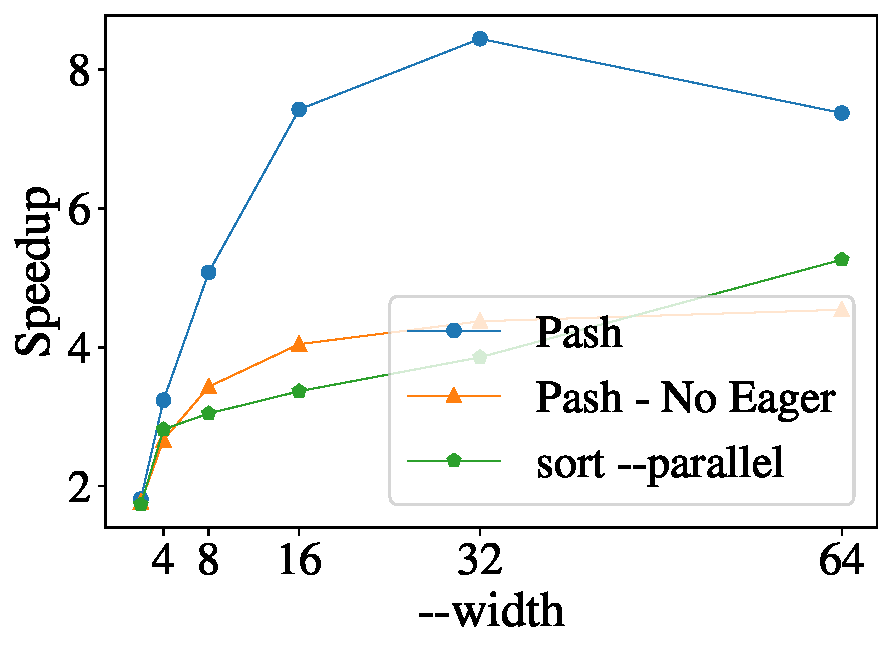
\includegraphics[width=0.25\textwidth]{\detokenize{./figs/sort_baseline_comparison_scaleup.pdf}}
  \end{center}
%   \vspace{-15pt}
% \caption{ \textbf{Comparison with \ttt{sort -{}-parallel}.} }
\end{wrapfigure}
Second, based on the comparison with \ttt{sort --parallel} it seems
that the scaleup limit that \sys reaches with sort is \todo{inherent
  and cannot be overpassed} \kk{We have to find a way to argue for the
  previous statement}. Because of that, all pipelines and scripts that
contain \ttt{sort} in our evaluation (several one-liners and unix50)
have this upper bound on scalability. \kk{Maybe move this paragraph in
  the one-liners section.}

Finally, this comparison showcases the benefit that \sys provides to
command developers. Instead of implementing a custom flag that enables
parallelism for a command, a simple specification of the command
parallelizability allows \sys to scale it similarly to a handcrafted
implementation with almost no effort.

%% \kk{There is a weird thing in the results. That the sequential one
%%   with --parallel=1 takes more than the \sys sequential one.}

\heading{GNU Parallel}
We compare \sys to \ttt{parallel} (v.20160422), a GNU utility for running other commands in parallel~\cite{Tange2011a}.
In the first experiment, we leverage \ttt{parallel}'s \ttt{--jobs} flag and redirect input from a file to 
Sequential execution takes \todo{XX}s, and \sys's parallel execution takes \todo{XX}s (speedup: \todo{XX}\%).
We note that this pipeline is harsh for \sys, in that most of the overhead comes from a single command---masking \sys's improvements in other parts of the pipeline.

% % https://github.com/marcelm/cutadapt/issues/157
% % https://www.biostars.org/p/123237/
% \begin{lstlisting}[language=sh, numbers=none]
% 	uniq | sort | parallel cutadapt-fastqc
% \end{lstlisting}
% % -S server01,server02 
% % -u -j24 --env PATH,PYTHONPATH,cutadapt_parallel
% % --workdir $PWD cutadapt_parallel {}

There are a few possible ways one might attempt to use GNU \ttt{parallel} to parallelize this program.
Assuming a user knows that the bottleneck comes from the \ttt{XX} stage, they could attempt to use \ttt{parallel} there.
This leads to a runtime of \todo{XX}s (speedup: \todo{XX}\%).

Alternatively, a user could (incorrectly) sprinkle \ttt{parallel} across the entire program;
  this is a common strategy simplified by \ttt{parallel}'s \ttt{stdin} redirection feature.
Doing this leads to \todo{XXX}\% performance improvements but severely incorrect results with respect to the sequential execution---a \ttt{diff} that averages about \todo{XX--XX} lines.
\sys's conservative program transformations will not attempt parallelizing program sections that contain commands with unclear \todo{parallelizability} properties.
	% or commands whose inputs depend on earlier outputs.
GNU \ttt{parallel} is oblivious to command semantics, risking breaking program semantics as in this case.

% Parallel is a great program for its target audience.

\heading{Manual Parallelization}
Alternatively, a user might attempt to manually parallelize individual commands by using the abstractions provided by the POSIX shell.
The benefits depend on several factors, such as whether a command is I/O- or CPU-bound.

\heading{Streaming Framework}
In a different attempt to identify how far \sys is from ideal performance, we start from programs already written in a high-performance parallel framework and rewrite as shell programs.
Raftlib~\cite{} is a C++ library enabling streaming and dataflow parallelism without the fault-tolerance overheads of distributed systems.
We rewrite three Raftlib benchmarks---\ttt{wordcount}, \ttt{XX}, and \ttt{XX}---as shell scripts.
% These benchmarks were relatively easy found relatively easy to port and match many of the workloads one would expect to see in the shell as shell pipelines.

\heading{Graph Transformations}
In the benchmarks, the overhead from \sys's analysis and generation phases remains collectively below $1s$ even for the high-scalability cases.
We decided to push \sys's limits by constructing an artificial 1000-stage pipeline---a worst-case workload that is nowhere near the ones observed in practice.
We find the resulting times quite acceptable:
  given two input arguments in the beginning of this pipeline, \sys takes $8.23s$ for parsing the script and $3.22s$ for analysis and optimization.
Pushing parallelization factor to $100\times$, \sys's runtime jumps to 5 minutes and 8 seconds to perform the analysis, producing an output dataflow graph that has more than 100 thousand edges in a file of about 11MB.

\heading{Take-aways}
\sys does not improve performance when running the risk of breaking correctness. % This should go in the intro
% Compared to \sys, \ttt{parallel} can lead to a combination of smaller performance improvements, incorrect execution with respect to the sequential program, and higher rewriting effort.
In highly-parallel benchmarks, \sys can lead to performance that is comparable to highly specialized streaming frameworks---at a fraction of the cost in terms of manual development.

\section{Related Work}
\label{related}

At a high level, techniques for re-writing programs to exploit parallelism fall under a wide spectrum that ranges from fully manual (but, ideally, optimal or more general) to fully automated (but potentially sub-optimal or specialized).
A significant concern with approaches that require user input is correctness:
   users---often neither experts in parallelism nor educated on the internals of the code they depend on---can easily break the semantics of sequential programs, especially when these depend on existing code (such as is the case with shell commands).

\heading{Parallel Shell Scripting}
Several utilities expose commands for specifying parallelism on modern \unix{}es---\eg \ttt{qsub}~\cite{gentzsch2001sun}, \textsc{SLURM}~\cite{yoo2003slurm}, calls to \textsc{GNU} \ttt{parallel}~\cite{Tange2011a}.
Different from \sys, their effectiveness is predicated upon explicit and careful invocation and is limited to embarrassingly parallel (and short) programs.
Often, these commands provide options to support an array of special sub-cases---a stark contradiction to the celebrated \unix philosophy.
For example, \ttt{parallel} contains flags such as \ttt{--skip-first-line}, \ttt{-trim}, and \ttt{--xargs}, that a \unix user can achieve using \ttt{head}, \ttt{sed}, and \ttt{xargs};
   it also introduces (and depends on) other programs with complex semantics, such as the ability transfer files between computers, separate text files, and parse CSV.
\sys embraces the \unix philosophy and simply attempts to rewrite pipelines more efficiently with minimal user effort---if any.

Several shells~\cite{duff1990rc, mcdonald1988support, dagsh:17} add primitives for non-linear pipe topologies---some of which target parallelism.
Here too, however, users are expected to manually rewrite scripts to exploit these new primitives, contrary to \sys.

Recently, the Smoosh authors have argued that certain shell features are useful for making concurrency explicit~\cite{smoosh:18}.
Their argument is somewhat antithetical to \sys, which argues that users should experience mostly automated (and correct) parallelization---hence \emph{light-touch} parallel scripting.


% Nice intro: http://homepages.inf.ed.ac.uk/bfranke/Publications/pldi121-tournavitis.pdf
\heading{Low-level Parallelization}
Instruction-level parallelization has a long history, starting from explicit \ttt{DOALL} and \ttt{DOACROSS} annotations~\cite{par1, par2} and continuing with compilers that attempt to automatically extract parallelism~\cite{padua1993polaris,hall1996maximizing}.
These systems operate at a lower level than \sys (\eg that of instructions or loops rather than the boundaries of programs that are part of a script), operating in a single target environment, and typically do not exploit high-level annotations.

More recent work focuses on extracting parallelism from domain-specific programming models~\cite{cilk5, streamIt, galois} and interactive parallelization tools~\cite{parascope, ipat}.
These tools simplify the expression of parallelism, but still require users to get involved in discovering and exposing parallelism.
% Moreover, the insights behind these attempts are significantly different from \sys's, as they extract parallelism statically during compilation instead of dynamically during runtime.
%Despite significant progress~\cite{}, it remains due to its need for complex program analysis and the unknown factors (such as input data range) during compilation.

\heading{Correct Parallelization of Dataflow Graphs}
The DFG is a prevalent model in several areas of data processing (including batch-~\cite{mapreduce:08, spark:12} and stream-processing ~\cite{murray2013naiad, carbone2015flink} systems).
Despite its popularity, most systems perform optimizations that do not preserve its semantics, introducing subtle erroneous behaviours.
Recent work~\cite{HSSGG2014, SHGW2015, MSAIT2019} attempts to address this issue by performing optimizations only in cases where correctness is preserved.
\sys draws inspiration from these efforts, as it attempts transformations that maintain the program's correctness with respect to the sequential execution.

\sys's proposed DFG model is diverges from prior works, as nodes it captures order.
This is due to the intricacies of the \unix model---its streams, its argument processing, and concatenation operators all maintain ordering.
% As a result, previous work is not directly applicable.

\heading{Parallel Userspace Environments}
By focusing on simplifying the development of distributed programs, a plethora of environments assist in the construction of parallel software.
Such systems~\cite{ousterhout1988sprite, mullender1990amoeba, pike1990plan9, barak1998mosix} or languages~\cite{erlang:96, acute:05, mace:07, cloudhaskell:11} hide many of the challenges of dealing with concurrency.
They do so as long as a program leverages the provided abstractions---which are strongly coupled to the underlying operating or runtime system.
A notable example is Plan9's \ttt{rc} shell that provided an interface for the construction of general programs.
Unfortunately these environments are not backward-compatible with the \unix shell, and often focus primarily on hiding the existence of a network---providing the illusion of a single-system image---rather than automatically accelerating scripts through parallel processing.
% simplify many of the problems of distribution and

\heading{Cluster Computing}
Several frameworks such as Phoenix~\cite{} and Raftlib~\cite{} offer full automation as long as their use leverages special primitives---\eg map-reduce-style primitives for Phoenix.
These primitives make strong assumptions about the nature of the computation---\eg strongly-eventual commutative functions that can proceed in parallel.
By targeting specific classes of computation (\emph{viz.} \sys's parallelizability), they can significantly optimize for their target domains.

% Lack of generality, no formal guaratees, their setup and is too tedious 
\sys chooses a more general approach: it does not require users to set up a new framework for every new class of computation they need to execute, nor to rewrite different parts of their computation using the specific abstractions provided by each framework they use.
It also takes a more principled approach: by developing the semantic model outlined earlier, it can focus on transformations that are correct with respect to the sequential program.

% % Although still a research prototype, \sys's setup and deployment is simpler.
% It also does not require these specialized frameworks, manually (re)write , and 
% Different from \sys, however, 
% Due to the specialization of these primitives, however, these systems suffer from a lack of generality ;
% % and they still require developers to compose their work using the pipelines
% Developing under these frameworks differs quite significantly from the development of normal (non-distributed) programs.

% \heading{Annotation-based Transformations}
% \sys inspiration from recent systems such as Ignis~\cite{ignis:19} and Mozart~\cite{mozart:19} which, as long as a developer has provided a few high-level annotations, they take care of automating scale-out.
% % Both work on high-level, managed languages---server-side JavaScript for Ignis and Python for Mozart---that allow runtime transformations without affecting the broader environment under which a program executes.
% These systems works on single-language, single-runtime environments 
% 
% For the critical points where user input is required, they provide a
% high-level declarative DSL with varying (but limited) degrees of
% expressive power.
% % Annotations are used by ---complicated by the use of third-party
% % libraries similar to \sys's extensions.
% Unfortunately, a challenge with this approach is that users composing
% applications by using third-party libraries do not understand their
% parallelizability details well-enough to annotate them.
% 
% \sys occupies a different point in the design space, by removing any work from composers and adding a small load to developers.
% % More specifically, it is designed to be used automatically by composers,
% Its DSL is designed to be more heavy-weight than Ignis' declarative recipes or Mozart's split annotations, but geared towards the developers of these components---not the users composing them.

% It also provides a more principled approach than both of these systems.
% Their annotations language is not as principled as \sys's---and one that is critical in ensuring that the dataflow analyses preserves the semantics expected by the developer
% The side-effects present in the shell dwarf those of functional languages



% https://ecommons.cornell.edu/bitstream/handle/1813/6508/85-668.pdf?sequence=1
% The growth of the web led to specialized frameworks for massively distributed computation~\cite{mapreduce:08, spark:10, naiad:13}.
% While they Moreover, these systems take advantage of functional purity;
%   for programs that are not data-intensive processing pipelines (\eg web servers), purely functional code is generally responsible for only a small fraction of the program runtime.

% \begin{figure}[t]
% \centering
% 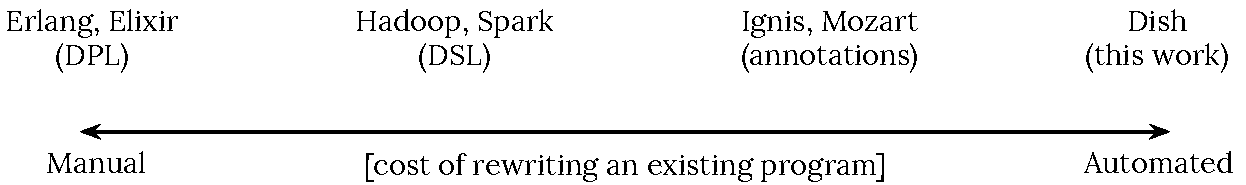
\includegraphics[width=0.49\textwidth]{\detokenize{./figs/dish_spectrum.pdf}}
% \caption{
%   \textbf{Manual--automated distribution spectrum.}
% 	\sys sits at the automation end of the spectrum, automatically distributing shell pipelines while maintaining their correctness.
% }
% \vspace{-15pt}
% \label{fig:spectrum}
% \end{figure}
% 

% \kk{exoume ena semantic model to opoio mporei na xrhsimopoiithei gia
%   na ginoun formally proven claims gia to equivalence preservation twn
%   optimizations etc.}

%% Possible points to add: These systems introduce data parallelism by
%% parallelizing nodes of the dataflow graph.  Unfortunately, they
%% often do not preserve the model's semantics, blurring the lines
%% between specification, optimization, and implementation.  In
%% contrast, \sys's dataflow model inherently supports the data
%% parallelism found in shell pipelines.  More specifically, it
%% develops a set of parallelization-exposing optimizations
%% represented as semantics-preserving graph transformations,
%% effectively exposing data parallelism as task parallelism.

%% \cite{HSSGG2014, SHGW2015} discuss optimizing transformations, but
%% their correctness is established using informal arguments based on
%% operational intution.
  
%% The paper \cite{MSAIT2019} proposes a denotational semantic framework
%% for stream processing where the data streams are seen as partial
%% orders, and establishes the soundness of some common parallelizing
%% transformations on dataflow graphs.

%% \km{Some very early references on the dataflow model of computation
%% (maybe there are relevant?): \cite{KM1966, D1974Dataflow, K1974KPN,
%% KMacQ1977}}
  


\section{Discussion \& Conclusion}
\label{discussion}

This paper presented \sys, a shell variant that parallelizes shell programs mostly automatically.
\sys's insight is that shell pipelines already express streaming computations that can be automatically distributed.
To achieve its goal, \sys
  decomposes primitives into parallelizability classes,
  identifies high-parallelizability stages,
  applies a series of transformations according to a DFG model,
  and orchestrates the execution of the parallel program.
% Its runtime component provides orchestration and planning support during the execution of the program.

\sys's current limitations revolve around shell expansion.
Currently, \sys does not attempt to parallelize program fragments for which variables have not been expanded.
Without substantial effort, \sys could be modified to at least suggest expansion of these fragments so that developers provide concrete values.
More significant effort would be required however to fully exploit latent parallelism in fragments that have not been expanding.
This effort would require tying \sys with the shell interpretation rather than having it as a compilation pass and is left for future work.

Despite limitation related to expansions, \sys can lead to significant benefits for shell users.
Experiments with real programs show substantial speedups and the ability to operate on large input datasets, all minimal or zero developer effort.


% \heading{Limitations}
% Our implementation is limited in many ways, so as to succeed in proving the key hypothesis---that scaling out shell pipelines can be automated and correct with respect to some assumptions.
% 
% \sys does not adequately handle failures or network partitions in the general sense, which would require re-scheduling passes on failed replicas.
% Prior work on fault-tolerant distributed stream processing can be of significant aid here.
% 
% The logic of the planner is quite simplified, attempting only straightforward placement of tasks to nodes (and using a hard-coded, homogeneous node structure).
% Prior work on operator placement of distributed dataflow graphs can be used to build a more sophisticated planner.
% 
% \sys is conservative in the shell subsets that it handles, in order to
% avoid introducing unsafe behaviours. The point of this work was not to be
% able to handle a complete distributable subset of the shell, but
% rather to use significant part of it to demonstrate performance benefits.
% 
% % Shell is highly dynamic, thus making it impossible to design sound
% % meaningful analyses to determine distributable regions and maximal
% % parallelization. In order to address this particularity, \sys could be
% % tighly integrated with a posix compliant shell
% % interpreter~\cite{smoosh:20} so that dynamic information can be
% % acquired selectively to aid the analysis and optimization process.
% 
% 
% \heading{Future Work}
% % \label{limitation}
% % \item No cycles (multiple commands writing and reading from the same file)
% There are several worthwhile directions for future work.  One
% direction would be an extension of the parallelizability analysis of
% \sys, in order to guide it using dynamic information. This could
% enable a formal study of the analysis~\sx{impl} to show that it
% returns regions that are safe to distribute.  Recent work on
% formalizing the semantics of the POSIX shell~\cite{smoosh:20} make
% such an attempt possible.
% 
% Another direction is to extend \sys to handle other classes outside \sta and \pur.
% These two classes enjoy a certain popularity with quick, one-off pipelines and are the easiest to distribute, but 
% it would be interesting to expand to \dfs (with the use of a distributed file-system) and \sid (with the use of transactional protocols).
% This direction would naturally introduce considerations about replication, consistency, and failure recovery.
% 
% There are two additional assumptions that have to be satisfied in
% order for the distributed implementation that is generated by Dish to
% have equivalent behaviour with the original implementation. First of
% all, there should be no external signals to the commands while they
% execute. At the moment Dish assumes no faults, and that communication
% always succeeds. This assumption can be lifted by extending Dish with
% a fault-tolerant runtime, \kk{blah blah}. Second, we assume that no
% command reads and writes to arbitrary files that are not mentioned in
% their arguments. This is a necessary assumption, since commands are
% considered as black boxes and the only information that can be
% inferred about them is through their arguments.

%% \begin{acks}
  % Dumping people so that we don't forget
  % 
  %% This material is based upon work supported by the
  %% \grantsponsor{GS100000001}{National Science
  %%   Foundation}{http://dx.doi.org/10.13039/100000001} under Grant
  %% No.~\grantnum{GS100000001}{nnnnnnn} and Grant
  %% No.~\grantnum{GS100000001}{mmmmmmm}.  Any opinions, findings, and
  %% conclusions or recommendations expressed in this material are those
  %% of the author and do not necessarily reflect the views of the
  %% National Science Foundation.
%% \end{acks}

%% Bibliography
\bibliography{./bib}


\appendix

\section{Annotation Language Grammar}
\label{alg}

\begin{figure}
  \centering
  \begin{grammar}
    <option> ::= `-' <string>

    <category> ::= `stateless' | `pure' | ...

    <maybe-int> ::= | <int>

    <arg> ::= `args[' <int> `]'

    <args> ::= <arg>
    \alt `args[' <maybe-int> `:' <maybe-int> `]'

    <input> ::= `stdin' | <args>

    <inputs> ::= <input>
    \alt <input> `,' <inputs>

    <output> ::= `stdout' | <arg>

    <option-pred> ::= <option>
    \alt `value' <option> = <string>
    \alt `not' <option-pred>
    \alt <option-pred> `or' <option-pred>
    \alt <option-pred> `and' <option-pred>

    <assignment> ::= `(' <category>, `[' <inputs> `]' , <output> `)'

    <predicate> ::= <option-pred> `=>' <assignment>

    <pred-list> ::= `|' <predicate> <pred-list>
    \alt `|' `otherwise' `=>' <assignment>

    <command> ::= <name> `\{' <pred-list> `\}'

    <command-list> ::= <command>
    \alt <command> <command-list>
  \end{grammar}
  \caption{
  \textbf{Parallelizability description language.}
    The DSL captures important information regarding the parallelizability of a command.
  }
  \label{fig:dsl}
\end{figure}

%% %% Appendix
%% \appendix
%% \section{Scripts used in the evaluation}

%% This appendix contains the source code of the scripts used in the evaluation of
%% the \sys. They are part of the codebase (released as open source with the camera
%% ready), and are provided here only to aid the reviewers.


\end{document}
